% AISTATS 2027 submission. Official unmodified 2027 style.
% Rewritten 2026-09-29 around the design-based WCS result. Every number in the
% main text traces to FACT_SHEET.md or to a table generated from the result CSVs.
\documentclass[twoside]{article}
\usepackage{aistats2027}
\usepackage[utf8]{inputenc}
\usepackage[T1]{fontenc}
\usepackage{amsmath,amssymb,amsthm,booktabs,graphicx}
\usepackage[numbers,sort&compress]{natbib}
\usepackage[hidelinks]{hyperref}
\newtheorem{theorem}{Theorem}
\newtheorem{corollary}{Corollary}
\newtheorem{proposition}{Proposition}
\newtheorem{lemma}{Lemma}
\newcommand{\FDP}{\operatorname{FDP}}
\newcommand{\FDR}{\operatorname{FDR}}
\newcommand{\Prb}{\mathbb{P}}
\newcommand{\E}{\mathbb{E}}
\newcommand{\ind}{\mathbf{1}}
\newcommand{\calset}{\mathcal{C}}
\newcommand{\testset}{\mathcal{T}}
\hypersetup{pdfauthor={},pdftitle={False Discovery Control Under Biased Label Acquisition on Graphs}}
\begin{document}
\raggedbottom
\setlength{\emergencystretch}{1.5em}
\twocolumn[
\aistatstitle{False Discovery Control Under Biased Label Acquisition on Graphs}
\aistatsauthor{Anonymous Authors}
\aistatsaddress{Anonymous Institution}
]
\begin{abstract}
Conformal $p$-values with the Benjamini--Hochberg (BH) procedure can flag anomalous nodes in a graph while controlling the false discovery rate (FDR), provided the verified-normal reference is a random sample of normal nodes. On graphs, labels are often acquired unevenly. On the Amazon, T-Finance and Weibo fraud graphs, selecting reference normals by their exposure to known anomalies, or acquiring labels with exposure-dependent probabilities, raises the false discovery proportion to as much as $0.29$ at a nominal level of $0.10$, even with accurate detectors. When acquisition probabilities are known, weighting each reference node by its inverse acquisition probability and applying weighted conformalized selection (WCS) restores control. We prove this using only the randomness of test assignment and label acquisition, so the guarantee allows dependence among nodes and holds when the detector is trained on part of the acquired labels. Across $18$ settings with retrained detectors, unweighted BH exceeds its bound in $15$, while WCS remains consistent with it at a power cost that is small under moderate bias and large under severe bias. When acquisition can be chosen, uniform acquisition at approximately the same expected label budget has higher power in every setting, so WCS is a correction for imbalance that cannot be avoided.
\end{abstract}

\section{INTRODUCTION}
A fraud team scores every account on a transaction graph and wants to flag suspicious accounts while keeping the false discovery rate (FDR) at a stated level. Conformal $p$-values with the Benjamini--Hochberg (BH) procedure give this guarantee when the reference set of verified normal accounts is a random sample of the normal accounts~\citep{bates2023testing}. On a graph that condition is easy to break. Which accounts get verified often depends on where they sit in the graph, for instance on how close they are to known fraud. The reference then represents some neighborhoods more than others. If the detector's score depends on neighborhood, normal test nodes from under-represented neighborhoods look anomalous next to the reference, and the guarantee fails with no visible sign in the output.

The failure is large even with accurate detectors. On three fraud graphs, removing the 20\% of reference normals most exposed to known anomalies raises the false discovery proportion (FDP) at nominal level $0.10$ from about $0.09$ to between $0.12$ and $0.29$, with scores, test nodes and reference size held fixed (Table~\ref{tab:threegraphs}). A filter of this kind gives the exposed normals zero acquisition probability, and without additional assumptions or information, inverse-probability correction cannot recover the guarantee for the full population. What can be repaired is acquisition in which every normal node keeps a positive, recorded probability of being verified. That case fails too: when labels are acquired with probabilities that depend on exposure and the detector is trained on those same labels, unweighted BH exceeds its FDR bound in 15 of 18 settings (Figure~\ref{fig:endtoend}).

The remedy uses the acquisition probabilities. If node $v$ was verified with a known probability $\rho(v)$, weight it by $1/\rho(v)$, the Horvitz--Thompson weight of survey sampling~\citep{horvitz1952generalization}, and run weighted conformalized selection (WCS)~\citep{jin2026weighted} on the weighted reference. Theorem~\ref{thm:design} shows that this controls FDR using only the randomness of which normal nodes are tested and which are labeled. Because the randomness comes from the design rather than from drawing nodes independently, the nodes may depend on one another in any way; what must hold is the design itself. Corollary~\ref{cor:trained} keeps the same weights when the scorer is trained on part of the acquired labels. Proposition~\ref{prop:wresolution} explains the price of sparse labeling: a node whose region was labeled with probability $\rho$ behaves, for discovery purposes, like a conformal test with roughly $\rho$ times the reference size.

Empirically, randomized WCS stays consistent with its bound in all 18 end-to-end settings, and the WCS procedure has a measured power cost. Against BH on the same randomized weighted $p$-values, which has no guarantee under this design, randomized WCS keeps at least $93\%$ of the power under moderate bias and between $28\%$ and $98\%$ under severe bias. That competitor showed no clear FDR violation in our runs; a three-node construction shows that it need not inherit the sharper $\alpha m_0/m$ guarantee, and its nominal validity under this design is unresolved. The method is not a reason to label unevenly: when acquisition can be chosen, uniform acquisition at approximately the same expected label budget had higher power in all 18 settings. With propensities estimated by a logistic model that uses the acquisition mechanism's predictors, a case the theorem does not cover, no clear violation was detected in our tests; with a misspecified propensity model control was lost.

What is new is the justification, not the procedure. The selection rule is the outlier-detection form of WCS, whose guarantee rests on independent draws under covariate shift~\citep{jin2026weighted}. Inverse-probability weighting is standard in finite-population sampling~\citep{horvitz1952generalization}. What requires a separate argument here is FDR control for WCS under the joint test-assignment, label-acquisition and training design. Theorem~\ref{thm:design} supplies it by replacing independent draws with that design, which is why dependence among nodes is allowed and why the design must hold as stated. Corollary~\ref{cor:trained} handles a step the existing analysis does not: when the scorer is trained on acquired labels, the scores depend on which nodes were acquired, and conditioning on the training set shows that the weights are unchanged. Our contributions are (i) matched evidence that reference selection and biased acquisition inflate false discoveries with accurate detectors; (ii) the finite-population guarantee and its training corollary; (iii) a resolution bound that locates the power loss; and (iv) an evaluation that measures the cost of the guarantee against an unguaranteed competitor, separates the two procedures' sharper guarantees with an explicit example, and compares against uniform acquisition at the same budget.

\paragraph{Relation to prior work.}
Conformal outlier testing with a shared reference gives BH FDR control under exchangeability~\citep{bates2023testing,vovk2005algorithmic}; AdaDetect extends this to learned scores~\citep{marandon2024adaptive}, and \citet{gazin2024transductive} analyze transductive conformal ranks. Weighted conformal inference handles covariate shift with density-ratio weights~\citep{tibshirani2019conformal}, and WCS turns weighted $p$-values into a selection procedure with FDR control under independent sampling~\citep{jin2026weighted}. Design-based conformal prediction applies survey weights to obtain coverage under complex sampling designs~\citep{wieczorek2023design,lee2026survey}. Those results concern the coverage of one prediction; we need FDR control across many simultaneous decisions on dependent nodes, which is where the WCS construction and our finite-population argument enter. Conditional calibration~\citep{fithian2022conditional} is the general principle behind the pruning step. \citet{hennhofer2026resolution} study the loss of resolution when conformal weights concentrate; Proposition~\ref{prop:wresolution} is the form this takes for selection under a labeling design. Graph conformal methods target prediction-set coverage~\citep{huang2023uncertainty,zargarbashi2023conformal,zargarbashi2024inductive,davis2025dynamic}, and conformal link prediction aligns calibration with the edge-observation mechanism~\citep{marandon2023link}. Robust-reference methods handle anomalies inside the reference~\citep{bashari2025robust}, a different intervention from biased selection among normals. Selection-conditional coverage~\citep{jin2025focal} and selection-aware conformal tests~\citep{wang2024selective} match reference and target selection; the stratified alternative in Appendix~\ref{app:stratified} applies that principle and loses power on our graphs.

\section{SETTING}
Let $s(v)$ be a fixed score for node $v$, larger for more anomalous nodes. A reference set $\calset$ contains $n$ verified normal nodes, disjoint from the $m$ test nodes $\testset$. The upper-tail conformal $p$-value is
\begin{equation}
p(v)=\frac{1+\sum_{u\in\calset}\ind\{s(u)\ge s(v)\}}{n+1}.
\label{eq:p}
\end{equation}
BH~\citep{benjamini1995controlling} rejects the $k$ smallest $p$-values, where $k$ is the largest index with $p_{(k)}\le\alpha k/m$, and rejects none if no such index exists. If $V$ of the $R$ rejected nodes are normal, $\FDP=V/(R\vee1)$ and $\FDR=\E[\FDP]$. Power is the fraction of anomalous test nodes rejected. Every mean we report includes runs with no rejections.

\paragraph{The random-sampling baseline.}
Condition on the graph, all labels, the scores and any labeled panel used to train the scorer. If the eligible normal nodes are assigned uniformly to reference and null-test positions, with ties broken by independent continuous marks drawn beforehand, then reference and null-test scores are exchangeable given the anomalous test scores. The conformal $p$-values are then super-uniform and positively regression dependent on the nulls (PRDS)~\citep[Theorem 3.3]{marandon2024adaptive}, and BH gives $\FDR\le\alpha m_0/m$, where $m_0$ is the number of null test nodes (Appendix~\ref{app:randomdesign}). The expectation is over the random partition. A reference chosen by a label-dependent filter, or one whose size depends on which nodes passed the filter, is outside this argument.

\paragraph{Resolution.}
Every $p$-value is at least $1/(n+1)$. Writing $r(v)=(n+1)p(v)$ and $N(r)=|\{v:r(v)\le r\}|$, BH rejects something exactly when some integer $r$ satisfies
\begin{equation}
N(r)\ge\frac{mr}{\alpha(n+1)},
\label{eq:crossing}
\end{equation}
so every nonempty rejection set has at least $\lceil m/[\alpha(n+1)]\rceil$ nodes (Appendix~\ref{app:proofs}). With $n=162$ reference nodes, $m=2{,}159$ test nodes and $\alpha=0.10$, this is 133 nodes. A small reference can suppress discoveries even when the detector ranks well.

\section{FDR CONTROL UNDER A LABEL-ACQUISITION DESIGN}
\label{sec:method}
\paragraph{Design.}
Condition on $\mathcal F$: the graph, all labels, a prior labeled panel, scores that do not depend on which normal nodes end up in the reference or the test set, independent continuous tie marks (so all scores are distinct), the anomalous test set $\testset_1$, and acquisition propensities $\rho(v)\in(0,1]$ that are functions of $\mathcal F$. Among the $N_0$ deployment normals, choose $m_0$ uniformly at random as null test nodes $\testset_0$, and acquire each remaining normal independently with probability $\rho(v)$. The acquired normals form the reference $\calset$. Write $w(v)=1/\rho(v)$, $\testset=\testset_0\cup\testset_1$ and $m=|\testset|$. The propensities are known when the team sets them before verifying, as in an audit that samples each region of the graph with a recorded probability; $\rho$ may depend on anything known beforehand, such as exposure to known fraud or degree. Labels produced by a process whose selection probabilities were never recorded are a harder case; Section~\ref{sec:results} reports one estimated-propensity setting that worked and one that failed.

\paragraph{Procedure.}
For a test node $j$ draw $U_j\sim\mathrm{Unif}(0,1)$ independently of everything else and set
\begin{equation}
\tilde p_j=\frac{U_j\,w(j)+\sum_{i\in\calset}w(i)\ind\{s(i)>s(j)\}}{w(j)+\sum_{i\in\calset}w(i)}.
\label{eq:randp}
\end{equation}
The deterministic $p$-value $p_j$ replaces $U_j$ by 1 and the strict inequality by $\ge$. For $l\neq j$ define the auxiliary values
\begin{equation}
p_l^{(j)}=\frac{\sum_{i\in\calset}w(i)\ind\{s(i)>s(l)\}+w(j)\ind\{s(j)>s(l)\}}{\sum_{i\in\calset}w(i)+w(j)},
\label{eq:aux}
\end{equation}
with $p_j^{(j)}=0$, and let $S_j$ be the number of BH rejections at level $\alpha$ among $(p_l^{(j)})_{l\in\testset}$; then $1\le S_j\le m$. The first stage keeps $\mathcal R_1=\{j:\tilde p_j\le\alpha S_j/m\}$. Homogeneous pruning draws one $\xi\sim\mathrm{Unif}(0,1)$, sets $r^*=\max\{r\in\{0,\ldots,m\}:|\{j\in\mathcal R_1:\xi S_j\le r\}|\ge r\}$ and reports $\mathcal R=\{j\in\mathcal R_1:\xi S_j\le r^*\}$; deterministic pruning uses $\xi=1$. This is the outlier-detection form of WCS, Algorithm~2 of \citet{jin2023algorithm}, with weights $1/\rho$. After one sort, all $S_j$ for test nodes sharing a weight value are computed in linear time, so the procedure costs one BH run per distinct weight.

\begin{theorem}[Design-based FDR control]
\label{thm:design}
Under the design above, WCS with weights $1/\rho$, deterministic or randomized $p$-values, and deterministic or homogeneous pruning satisfies $\E[\FDP\mid\mathcal F]\le\alpha m_0/m\le\alpha$.
\end{theorem}
The proof is in Appendix~\ref{app:wcsdesign}. Its core is a swap argument. Fix a null test position and condition on everything except which member of $\mathcal S=\calset\cup\{\text{that node}\}$ occupies it. Each candidate $j$ requires every other member of $\mathcal S$ to have been acquired, so the configuration has probability proportional to $\prod_{i\in\mathcal S\setminus\{j\}}\rho(i)$, and $\Prb(\text{position holds }j)\propto1/\rho(j)=w(j)$. Under this law the deterministic $p$-value is super-uniform and the randomized one is exactly uniform, while $S_j$ is the same for every candidate because the auxiliary values depend only on the multiset $\mathcal S$. The pruning step then bounds each null node's contribution to the FDP by $\alpha/m$, and summing over the $m_0$ null positions gives the bound. The argument adapts the weighted-exchangeability proof of \citet{jin2026weighted}, which assumes independent draws under covariate shift, to a finite population with a known sampling design. Nothing in it is specific to graphs; graphs are where the independence assumption fails and where exposure-dependent labeling arises.

\begin{corollary}[Scorer trained on acquired labels]
\label{cor:trained}
Fix $f\in[0,1)$. Suppose each acquired node is sent to a training set with probability $f$ and otherwise to the reference, and the scorer may depend on the training set, the prior panel, fixed graph information and independent model randomness. Then the conclusion of Theorem~\ref{thm:design} holds with the same weights $1/\rho$. With node-dependent fractions $f(v)$ the weights become $1/\{\rho(v)(1-f(v))\}$.
\end{corollary}
Conditioning on the training set fixes the scores, and the swap law picks up a common factor $1/(1-f)$ that cancels (Appendix~\ref{app:wcsdesign}). This is the setting of our end-to-end experiments, where a single biased acquisition supplies both the training labels and the reference.

\paragraph{What the guarantee needs.}
The propensities must be the true ones, known and positive; test normals must be chosen uniformly given their count; acquisition must be independent across nodes given $\rho$; scores must not depend on the roles of normal nodes beyond the training set of the corollary. The theorem does not cover propensities estimated after the fact, acquisition that adapts to labels as they arrive, or a filter applied to the reference after acquisition. Section~\ref{sec:results} reports what happens empirically with estimated propensities, including a misspecified model.

\paragraph{Filters versus probabilistic acquisition.}
A deterministic filter, such as removing the most exposed normals in Table~\ref{tab:threegraphs}, sets $\rho=0$ for the removed nodes. Without additional assumptions or information, inverse-probability correction cannot recover the full-population guarantee when some nodes have zero acquisition probability, because the reference then carries no information about the region the filter removed. The remedy changes the procedure rather than the analysis: instead of discarding exposed normals, keep each with a small known probability and weight it by $1/\rho$. The moderate and severe acquisition designs of Section~4 do exactly this, retaining the most exposed fifth of nodes with probability $0.10$ or $0.025$ instead of $0$.

\begin{proposition}[Weighted resolution]
\label{prop:wresolution}
Let $f_j=w(j)/\{w(j)+\sum_{i\in\calset}w(i)\}$, the smallest value the deterministic $p$-value of $j$ can take. If $j$ is rejected by weighted BH or by WCS with deterministic $p$-values and deterministic pruning, then $|\mathcal R|\ge mf_j/\alpha$; with homogeneous pruning, $|\mathcal R|\ge\xi mf_j/\alpha$. No node with $f_j>\alpha$ is rejected by any of these procedures.
\end{proposition}
Under the design, $\E[\sum_{i\in\calset}w(i)\mid\mathcal F,\testset_0]$ equals the number $N_{\rm ref}$ of non-test normals whatever the propensities are. Plugging in this mean gives $f_j\approx1/\{1+\rho(j)N_{\rm ref}\}$, so for discovery a node acquired with probability $\rho(j)$ behaves like an unweighted conformal test with $\rho(j)N_{\rm ref}$ reference nodes, and Equation~\eqref{eq:crossing} applies with $n=\rho(j)N_{\rm ref}$. This is an interpretation, not a concentration statement; with very small propensities the weighted mass varies. When anomalies concentrate in a sparsely labeled stratum, every discovery there with deterministic $p$-values needs many simultaneous rejections. Randomization replaces the hard floor by $U_jf_j$: conditional on everything except $U_j$, the first-stage rejection probability is $\min\{1,\max\{0,(t-b_j)/f_j\}\}$ with $t=\alpha S_j/m$ and $b_j$ the reference mass above $s(j)$, so a node can be rejected below the deterministic floor, with a probability that still depends on $b_j$.

An alternative remedy calibrates each exposure stratum against its own acquired normals and splits $\alpha$ across strata (Lemma~\ref{lem:stratified}, Appendix~\ref{app:stratified}). It is valid under the same design but loses power on our graphs, and we report it as a comparison.

\section{EXPERIMENTAL DESIGN}
\paragraph{Graphs and scorers.}
Amazon has 11,944 nodes, of which 7,818 are verified normal and 821 anomalous; its first 3,305 nodes carry no label and are excluded from reference and evaluation~\citep{dou2020enhancing,dglfraud}. T-Finance has 39,357 nodes and 1,803 anomalies, and Weibo has 8,405 nodes and 868 anomalies in the GADBench release~\citep{tang2023gadbench}; the PyGOD release of the same Weibo graph marks only 347 anomalies, so we treat the two as separate sources (Appendix~\ref{app:extensions}). Tolokers~\citep{platonov2023critical} yields almost no power for any rule and is reported in the appendices, as are the unsupervised detectors DOMINANT~\citep{ding2019deep}, GAE~\citep{liu2024pygod} and Isolation Forest~\citep{liu2008isolation}. The main scorers are histogram gradient-boosting classifiers with fixed settings (Appendix~\ref{app:supervised}), trained on a uniform 10\% prior panel of labeled nodes, using either node attributes alone or attributes plus the neighbor-mean attributes and log degree. Ten training seeds each draw a panel; five label-stratified splits assign about 25\% of the remaining nodes to testing. On the labeled population the scorers reach AUROC 0.969 and 0.971 on Amazon, 0.940 and 0.962 on T-Finance, and 0.982 and 0.993 on Weibo.

\paragraph{Reference selection.}
Exposure is the fraction of a node's neighbors known to be anomalous from the prior panel and from a revealed fraction of the non-test labels. The zero-exposure rule keeps only reference normals with no known anomalous neighbor. The graded rule removes the fraction $d\in\{0,.05,.10,.20,.40,.60,.80,.90,.97\}$ of reference normals with the highest exposure, breaking ties at random, and compares with removing the same number uniformly at random, over 50 paired repetitions. Scores, test nodes and reference size are identical within a pair. The designated comparison, fixed in the protocol before any T-Finance result was computed, removes 20\% with half of the non-test labels revealed.

\paragraph{Biased acquisition.}
Exposure strata are fixed from the prior panel alone: the lower 80\% and upper 20\% of exposure ranks over the deployment nodes, with independent tie marks. Non-test nodes are then acquired independently with probability $0.50$ in the lower stratum and $0.10$ (moderate) or $0.025$ (severe) in the upper stratum. A third, smooth design sets $\rho(v)=\operatorname{clip}_{[0.01,0.95]}\{\operatorname{sigmoid}(-1.2\sqrt{k_v}+0.3z_v)\}$, where $k_v$ counts panel-labeled anomalous neighbors and $z_v$ is standardized log degree. In the end-to-end version each acquired node goes to training with probability $1/2$ and otherwise to the reference; the scorer is retrained on the prior panel plus the acquired training labels, so both the scores and the reference depend on the biased acquisition, as in Corollary~\ref{cor:trained}. We compare BH on the acquired reference without weights; weighted BH with weights $1/\rho$, on deterministic and on randomized $p$-values; WCS with deterministic $p$-values; and randomized WCS, the last two with homogeneous pruning. Ten seeds, five splits and three acquisition draws give 150 runs per cell; the known-propensity experiments on frozen scores use ten acquisition draws. Each biased design is also compared with uniform acquisition at a rate fixed before test assignment, the mean prescribed probability over the deployment population, so that expected label budgets approximately match (Appendix~\ref{app:uniform}).

\paragraph{Estimated propensities.}
Under the smooth design we also replace $\rho$ by an estimate fitted to the acquisition indicators of the non-test nodes, a cross-fitted logistic regression on $\sqrt{k_v}$, $k_v$, log degree and exposure, and by a deliberately misspecified estimate, the empirical acquisition rate within each of the two exposure strata.

\paragraph{Metrics and uncertainty.}
All tests use $\alpha=0.10$. We average FDP and power over splits and acquisition draws within each training seed and report the mean over the ten seeds. Seeds are the independent units; the splits within a seed share its prior panel. Intervals in figures are pointwise 95\% $t$ intervals over the ten seed averages. They describe repeated evaluation of a fixed graph, not uncertainty over new graphs, and a sample mean below the bound is not evidence of control; the theorem is.

\paragraph{Protocols.}
Each experiment's protocol, including its seeds, arms and comparison rule, was written and hashed before its outcomes were seen, and the follow-up experiments (WCS, randomized $p$-values, estimated propensities, end-to-end retraining, the search behind Appendix~\ref{app:wbhcounter} and the uniform comparison) were chosen after inspecting earlier results. The pre-set rule for carrying WCS into the main text, power within $0.05$ of weighted BH at moderate bias on T-Finance and Weibo, was met by homogeneous pruning and not by deterministic pruning; both are reported. The supplement contains the protocols, code, per-trial ledgers and a script that reproduces the main results from a fresh copy.

\section{RESULTS}
\label{sec:results}
\begin{table*}[t]
\centering\small\setlength{\tabcolsep}{5pt}
\caption{Moderate reference selection with useful scorers on three graphs. Half of non-test labels are revealed; the highest-exposure 20\% of reference normals are removed, or the same count is removed randomly. Scores, test identities and remaining reference sizes match within each pair. Entries give mean FDP / power at nominal $0.10$. The final column gives the paired FDP increase in percentage points with a pointwise 95\% interval over ten seed averages, conditional on each graph. All abstentions are included.}
\label{tab:threegraphs}
\begin{tabular}{llrrl}\toprule
Graph & Score & Exposure & Random & $\Delta$ FDP (pp) [95\% interval]\\\midrule
Amazon & Attributes & $0.119/0.799$ & $0.088/0.778$ & $+3.1\ [2.2,4.0]$ \\
Amazon & Graph features & $0.145/0.820$ & $0.091/0.788$ & $+5.4\ [3.9,6.9]$ \\
T-Finance & Attributes & $0.127/0.668$ & $0.093/0.650$ & $+3.4\ [2.4,4.3]$ \\
T-Finance & Graph features & $0.191/0.830$ & $0.095/0.789$ & $+9.6\ [7.7,11.6]$ \\
Weibo (GADBench) & Attributes & $0.184/0.783$ & $0.094/0.663$ & $+9.0\ [7.5,10.6]$ \\
Weibo (GADBench) & Graph features & $0.286/0.973$ & $0.091/0.844$ & $+19.5\ [18.0,21.1]$ \\
\bottomrule\end{tabular}
\end{table*}


\paragraph{Filtering the reference inflates false discoveries.}
Table~\ref{tab:threegraphs} gives the designated comparison. Removing the most exposed 20\% of reference normals raises mean FDP on every graph and for both scorers, from $0.088$ to $0.119$ and from $0.091$ to $0.145$ on Amazon, from $0.093$ to $0.127$ and from $0.095$ to $0.191$ on T-Finance, and from $0.094$ to $0.184$ and from $0.091$ to $0.286$ on Weibo. Every paired interval excludes zero. Random references already achieve power between $0.65$ and $0.84$, so these are changes to a useful pipeline. The oracle zero-exposure rule on Amazon gives FDP $0.192$ against $0.067$ for a random reference of the same size (Appendix~\ref{app:supervised}), and Appendix~\ref{app:dose} reports the full dose curves. In 2,000 simulated graphs, a score that depends on degree is enough to produce the failure: with heterogeneous degree and strong cross-class connectivity the zero-exposure filter gives FDP $0.751$ against $0.061$ for random calibration, while degree-insensitive scores give at most $0.081$ (Appendix~\ref{app:indgraphs}). Weak unsupervised detectors show larger contrasts, which we keep in Appendix~\ref{app:unsupervised} because they do not describe a useful detector.

\begin{figure*}[t]
\centering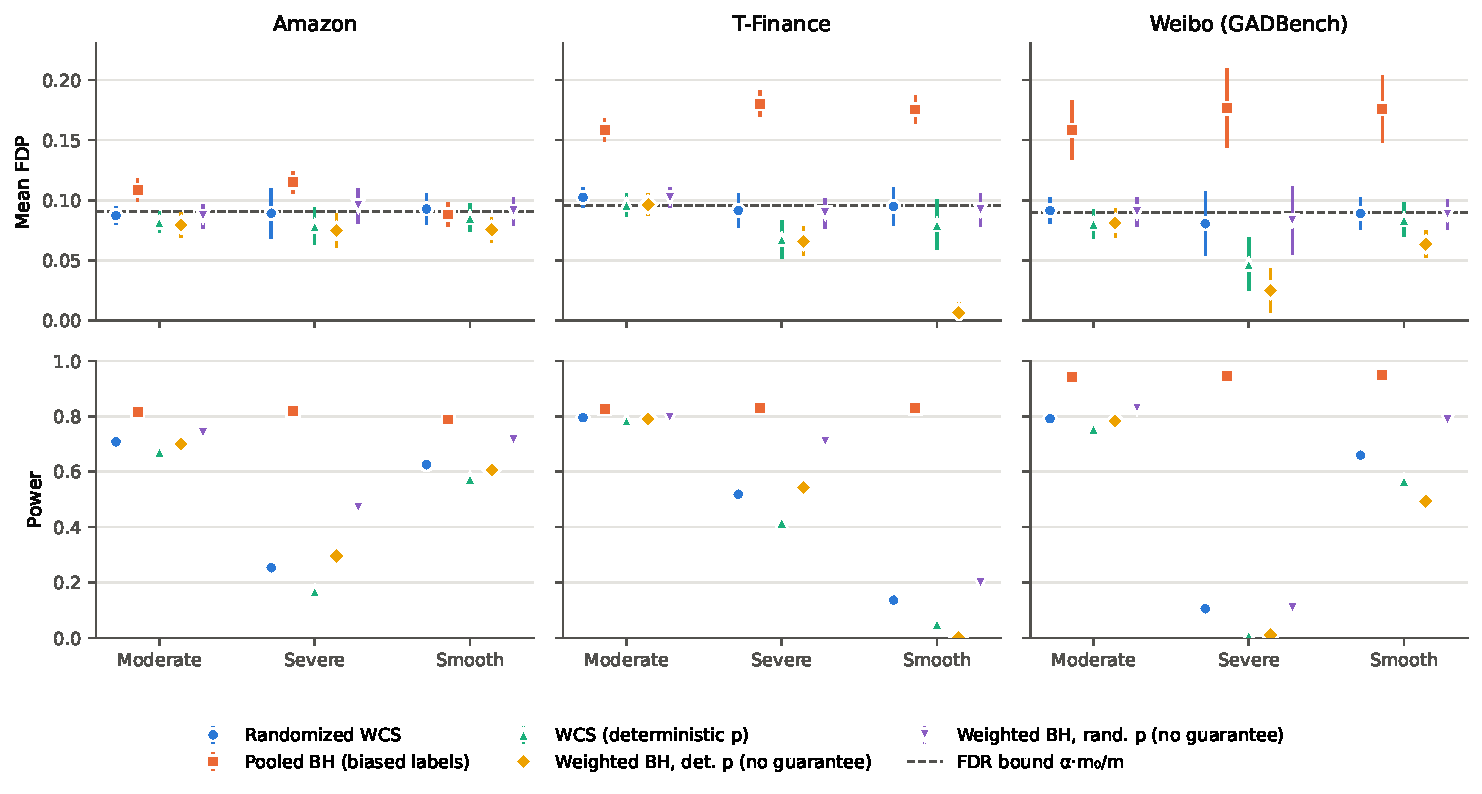
\includegraphics[width=\textwidth]{wcs_endtoend_figure.pdf}
\caption{Biased label acquisition with the scorer retrained on the acquired labels (graph-feature scorer; the attribute scorer is in Appendix~\ref{app:wcsdesign}). Top: mean FDP; bottom: power. Each point averages ten training seeds, five test splits and three acquisition draws; FDP bars are pointwise 95\% $t$ intervals over the ten seed averages. The dashed line is the bound $\alpha m_0/m$. Weighted BH, with deterministic or randomized $p$-values, has no FDR guarantee in this setting. Intervals that span the bound do not establish control; Theorem~\ref{thm:design} does.}
\label{fig:endtoend}
\end{figure*}

\paragraph{Biased acquisition breaks BH; WCS keeps control.}
Hard filtering gives some nodes zero acquisition probability, so the rest of this section turns to probabilistic acquisition, in which every normal node keeps a positive probability of being labeled. Figure~\ref{fig:endtoend} and Table~\ref{tab:endtoend} (Appendix~\ref{app:wcsdesign}) give the end-to-end results. Unweighted BH on the acquired reference exceeds its bound by more than two seed-clustered standard errors in 15 of the 18 settings, reaching FDP $0.180$ on T-Finance under severe bias against a bound of $0.095$. The three exceptions are the smooth design on Amazon, with both scorers, and on T-Finance with the attribute scorer, where the sample means ($0.088$, $0.090$ and $0.101$) sit near the bound. Randomized WCS is consistent with the bound in every setting. Its largest upward deviation is $1.9$ standard errors (T-Finance, graph scorer, moderate bias, mean $0.102$ against $0.095$), and no other cell exceeds the bound by more than $1.6$.

\paragraph{Power cost of the WCS procedure.}
The like-for-like comparison is BH on the same randomized weighted $p$-values, computed from the same scores, reference, test nodes, weights and auxiliary uniforms. Its validity under this design is unresolved. Its largest mean FDP is $0.103$, $1.8$ standard errors above the bound, so no clear violation was detected in these runs. A three-node construction shows that randomized weighted BH need not inherit the sharper $\alpha m_0/m$ guarantee (Appendix~\ref{app:wbhcounter}), although neither this example nor our benchmark experiments establishes a violation of nominal FDR control. Under moderate bias randomized WCS gives up between $0.000$ and $0.048$ in power to it. Under severe bias the gap reaches $0.348$ on T-Finance with the attribute scorer ($0.138$ against $0.486$) and about $0.2$ on Amazon with either scorer, while on Weibo both procedures have low power. Because both procedures use the same weights and $p$-values, the loss comes from the WCS selection procedure (its first-stage thresholds and its pruning); we have not separated the two. Against weighted BH with deterministic $p$-values, randomized WCS has higher power in 13 of 18 settings, and it has at least the power of WCS with deterministic $p$-values in all 18. Against the unguaranteed unweighted procedure the moderate-bias cost is small on T-Finance ($0.796$ against $0.828$, graph scorer) and larger on Weibo ($0.792$ against $0.943$). On Amazon under the smooth design unweighted BH happened to stay at the bound, and the correction cost about $0.16$ in power; the weighting is insurance whose premium is paid whether or not the bias would have hurt. The retrained scorers have AUROC between $0.939$ and $0.994$, so these losses occur despite accurate overall ranking.

\begin{table}[t]
\centering\small
\caption{Power of randomized WCS under each biased design $\to$ under uniform acquisition at approximately matched expected label budgets (graph-feature scorer; expected counts differ by at most $2.2$ labels). Every paired difference is positive with a seed-clustered 95\% interval above zero, for both scorers (Table~\ref{tab:uniform}).}
\label{tab:uniformmain}{\setlength{\tabcolsep}{3pt}\begin{tabular}{lccc}
\toprule
Graph & Moderate & Severe & Smooth\\
\midrule
Amazon & 0.71 $\to$ 0.80 & 0.25 $\to$ 0.80 & 0.63 $\to$ 0.79\\
T-Finance & 0.80 $\to$ 0.81 & 0.52 $\to$ 0.80 & 0.14 $\to$ 0.80\\
Weibo & 0.79 $\to$ 0.91 & 0.11 $\to$ 0.90 & 0.66 $\to$ 0.91\\
\bottomrule
\end{tabular}
}
\end{table}

\paragraph{Uniform acquisition at the same budget has higher power.}
If the team can choose the acquisition probabilities, it can avoid the imbalance altogether. At approximately the same expected label budget (expected counts differ by at most $2.2$ labels, $0.06\%$), randomized WCS under uniform acquisition had higher power than under the matched biased design in all 18 settings, by $0.012$ to $0.116$ under moderate bias and $0.29$ to $0.80$ under severe bias, with every seed-clustered 95\% interval above zero (Table~\ref{tab:uniformmain}; both scorers in Table~\ref{tab:uniform}). Its FDP stayed near the bound, with the largest upward deviation $2.5$ standard errors (T-Finance, $0.101$ against $0.095$). Under our biased designs nodes near known anomalies are labeled less often, so uniform acquisition also gives the scorer more training anomalies (for example $206$ against $122$ on Weibo) and avoids the sparse, heavily weighted stratum that limits resolution; we have not separated these two contributions.

\begin{table*}[t]
\centering\small
\caption{Smooth acquisition design with the true, estimated and misspecified propensities: mean FDP / power at nominal $0.10$ over ten seeds, five splits and ten acquisition draws on frozen scores. The estimate is a cross-fitted logistic regression on the acquisition indicators; the misspecified estimate uses two stratum rates. Theorem~\ref{thm:design} covers only the true-$\rho$ column.}
\label{tab:estimated}\begin{tabular}{llcccc}
\toprule
Graph & Scorer & Pooled BH & WCS, true $\rho$ & WCS, estimated $\rho$ & WCS, 2-stratum $\hat\rho$\\
\midrule
Amazon & Graph & 0.091 / 0.788 & 0.090 / 0.706 & 0.089 / 0.696 & 0.080 / 0.769\\
Amazon & Attr. & 0.090 / 0.781 & 0.088 / 0.700 & 0.087 / 0.694 & 0.085 / 0.759\\
T-Finance & Graph & 0.169 / 0.823 & 0.093 / 0.252 & 0.092 / 0.242 & 0.157 / 0.817\\
T-Finance & Attr. & 0.100 / 0.655 & 0.091 / 0.177 & 0.094 / 0.185 & 0.097 / 0.650\\
Weibo (GADBench) & Graph & 0.183 / 0.942 & 0.092 / 0.754 & 0.090 / 0.720 & 0.139 / 0.905\\
Weibo (GADBench) & Attr. & 0.137 / 0.728 & 0.093 / 0.572 & 0.090 / 0.539 & 0.118 / 0.688\\
\bottomrule
\end{tabular}

\end{table*}

\paragraph{Estimated propensities: one favorable case, one failure.}
Table~\ref{tab:estimated} replaces the true propensities by estimates. With a logistic estimator that uses the acquisition mechanism's predictors (the generating probabilities are additionally clipped, so the fitted family is close to but not exactly the true one), no clear violation was detected in the six cells, and power is within $0.035$ of the true-$\rho$ procedure. This is one estimator under one constructed mechanism, and Theorem~\ref{thm:design} does not cover it. With two stratum rates fitted to a smooth mechanism, control is lost on T-Finance ($0.157$, graph scorer) and Weibo ($0.139$ and $0.118$). The propensity model must describe how labels were actually acquired; being fixed in advance is not enough. On T-Finance the smooth design pushes $\rho$ down to $0.01$ for the most exposed nodes, and randomized WCS has power between $0.18$ and $0.25$ there with true or estimated propensities, which the next paragraph explains.

\paragraph{Resolution explains where power is lost.}
For deterministic $p$-values, Proposition~\ref{prop:wresolution} gives the required rejection count $mf_j/\alpha$ for an anomaly in the sparse stratum; homogeneous pruning scales it by $\xi$, and randomized $p$-values relax it. On the frozen-score experiments with the 80/20 strata it rises from about 7 with uniform acquisition to 35--37 under moderate bias and 140--148 under severe bias, in proportion to $1/\rho$ (Appendix~\ref{app:wcsdesign}, Table~\ref{tab:resolution}). Anomalies concentrate in that stratum: 51\% of test anomalies on Amazon, 88\% on T-Finance and 91\% on Weibo. Randomization relaxes the floor, and under severe bias it raises the power of WCS from $0.160$ to $0.331$ on Amazon, from $0.730$ to $0.766$ on T-Finance and from $0.197$ to $0.345$ on Weibo. Across 39,207 nonempty rejection sets in these experiments, no rejection violated the bound of the proposition.

\paragraph{Other remedies and diagnostics.}
Calibrating each exposure stratum against its own normals with $\alpha$ split across strata is valid under the same design but weaker: on Amazon, power falls from $0.779$ to $0.651$ for the attribute scorer, because most anomalies sit in the small high-exposure stratum (Appendices~\ref{app:stratified} and~\ref{app:allocation}). On a labeled development graph, the null rank under a uniformly drawn reference is hypergeometric, so the effect of a reference rule on null ranks can be computed exactly; a rule can shift null ranks while producing few discoveries, because the crossing in Equation~\eqref{eq:crossing} is rarely reached (Appendix~\ref{app:rankaudit}).

\section{DISCUSSION AND LIMITATIONS}
The results suggest an order of preference. A team that controls how labels are acquired and has no reason to favor some nodes should acquire uniformly: at approximately the same expected budget this had higher power in every setting we tested, and ordinary conformal BH is then valid. When acquisition probabilities are unequal, the team should decide them before verifying, record them, verify independently, and calibrate with WCS on the $1/\rho$-weighted reference; the scorer may be trained on part of the acquired labels. Before spending the budget, the plug-in form of Proposition~\ref{prop:wresolution} gives an approximate count of the simultaneous rejections a discovery in each stratum will need, a planning diagnostic for whether a stratum is labeled too sparsely to be useful; the exact bound depends on the realized reference mass and, with homogeneous pruning, on $\xi$. A filter that removes nodes from the reference should be replaced by probabilistic acquisition: acquire those nodes with a smaller but known positive probability and weight them by $1/\rho$, so rarely acquired nodes receive larger weights.

The guarantee has boundaries. It averages over the random choice of test nodes and is not a guarantee for an arbitrarily chosen deployment batch. It requires the true acquisition probabilities: estimated probabilities performed well in the tested setting but are not covered, a misspecified model lost control (Table~\ref{tab:estimated}), and labels whose selection probabilities were never recorded remain an open case. Acquisition that adapts to labels as they arrive is not covered. Under severe bias randomized WCS has substantially less power than randomized weighted BH, whose nominal validity under this design is unresolved; we have not shown that every procedure with a guarantee must pay this cost. We did not measure verification costs, so settings in which unequal acquisition is cheaper per label or otherwise required motivate future evaluation rather than being assumed here. Randomized decisions depend on auxiliary coins, which some practitioners will not accept, and deterministic $p$-values pay for determinism in power. The acquisition mechanisms are simulated on public benchmarks, the scorers are gradient-boosted classifiers rather than graph neural networks, the pipeline starts from a uniform 10\% prior panel whose labels count toward the budget, and the two Weibo releases disagree about which nodes are anomalous. Seed intervals describe repeated evaluation of one graph, not new graphs. Finally, the argument does not use the graph structure, which makes it portable to any finite population with a known labeling design.

\clearpage
\section*{AI Use Statement}
Generative AI tools assisted with designing the score and graph simulations, the conditional rank audit and the weighted-selection experiments; with formulating and revising mathematical statements and proofs, including the design-based guarantee and its corollary; with implementing validation code; with interpreting experimental results; with generating tables and figures; and with drafting, restructuring and editing the manuscript. Synthetic observations were generated by the specified random sampling programs and every reported numerical result comes from executed code that is included in the supplement. Bibliographic claims were checked against primary sources. The authors remain responsible for the content and reviewed all AI-assisted proofs, code, interpretations and writing before submission.
\bibliographystyle{plainnat}
\bibliography{aistats_refs}

\clearpage\section*{Checklist}
\begin{enumerate}

  \item For all models and algorithms presented, check if you include:
  \begin{enumerate}
    \item A clear description of the mathematical setting, assumptions, algorithm, and/or model. [Yes. Sections 2--4 define the setting, the acquisition design, the procedure and the experiments; Appendices~\ref{app:wcsdesign}, \ref{app:supervised} and~\ref{app:certificate} give the complete statements.]
    \item An analysis of the properties and complexity (time, space, sample size) of any algorithm. [Partial. Section 3 states the cost of the procedure (one sort, then one BH run per distinct weight value, so up to quadratic work when every test node has its own weight) and Proposition~\ref{prop:wresolution} gives the sample-size requirement for a discovery; no full complexity analysis of every baseline is provided.]
    \item (Optional) Anonymized source code, with specification of all dependencies, including external libraries. [Yes. The anonymized supplement includes the source, pinned dependencies, frozen protocols, per-trial ledgers and a verification script.]
  \end{enumerate}

  \item For any theoretical claim, check if you include:
  \begin{enumerate}
    \item Statements of the full set of assumptions of all theoretical results. [Yes. Section 3 states the assumptions of Theorem~\ref{thm:design}, Corollary~\ref{cor:trained} and Proposition~\ref{prop:wresolution}, including what they do not cover; Appendices~\ref{app:proofs}, \ref{app:stratified}, \ref{app:allocation} and~\ref{app:certificate} state the assumptions of the remaining results.]
    \item Complete proofs of all theoretical results. [Yes. Appendix~\ref{app:wcsdesign} proves the design-based guarantee, its corollary and the resolution proposition; Appendix~\ref{app:proofs} proves the score-level and resolution statements; Appendix~\ref{app:stratified} proves the stratified lemma; Appendix~\ref{app:allocation} proves the allocation variants; Appendix~\ref{app:certificate} proves the batch certificate.]
    \item Clear explanations of any assumptions. [Yes. Known versus estimated propensities, independent acquisition, uniform test assignment, role-invariant scores, tie conventions and fixed-batch conditioning are distinguished.]
  \end{enumerate}

  \item For all figures and tables that present empirical results, check if you include:
  \begin{enumerate}
    \item The code, data, and instructions needed to reproduce the main experimental results (either in the supplemental material or as a URL). [Yes. The supplement contains the scripts, processed inputs or acquisition instructions, cached scores, per-trial outcomes and a script that reproduces the main results from a fresh copy (Appendix~\ref{app:implementation}).]
    \item All the training details (e.g., data splits, hyperparameters, how they were chosen). [Yes. Section 4 and Appendices~\ref{app:implementation}, \ref{app:supervised}, \ref{app:dose} and~\ref{app:extensions} give the fixed settings, panel and split construction, and acquisition designs; follow-up experiments are identified as such.]
    \item A clear definition of the specific measure or statistics and error bars (e.g., with respect to the random seed after running experiments multiple times). [Yes. Section 4 and the captions define FDP, power, the averaging order, seed-clustered intervals, Monte Carlo SEs and paired intervals, and state what each does and does not measure.]
    \item A description of the computing infrastructure used. (e.g., type of GPUs, internal cluster, or cloud provider). [Yes. Appendix~\ref{app:implementation} describes the GPU used for the unsupervised detectors and the CPU environment for every other experiment.]
  \end{enumerate}

  \item If you are using existing assets (e.g., code, data, models) or curating/releasing new assets, check if you include:
  \begin{enumerate}
    \item Citations of the creator If your work uses existing assets. [Yes. Dataset, model and statistical-method sources are cited.]
    \item The license information of the assets, if applicable. [No. Source provenance and hashes are recorded, but a consolidated inventory of asset licenses is not included.]
    \item New assets either in the supplemental material or as a URL, if applicable. [Yes. New code, protocols, cached scores, synthetic results and validation outputs are in the supplement.]
    \item Information about consent from data providers/curators. [No. We reuse public benchmark releases and did not collect new provider-consent information.]
    \item Discussion of sensible content if applicable, e.g., personally identifiable information or offensive content. [Not Applicable. The experiments use released numerical graph data and synthetic observations; no new personally identifying or offensive content is curated.]
  \end{enumerate}

  \item If you used crowdsourcing or conducted research with human subjects, check if you include:
  \begin{enumerate}
    \item The full text of instructions given to participants and screenshots. [Not Applicable. We did not recruit participants or conduct a new human-subject study.]
    \item Descriptions of potential participant risks, with links to Institutional Review Board (IRB) approvals if applicable. [Not Applicable. We did not recruit participants or conduct a new human-subject study.]
    \item The estimated hourly wage paid to participants and the total amount spent on participant compensation. [Not Applicable. We did not recruit participants or conduct a new human-subject study.]
  \end{enumerate}

\end{enumerate}

\clearpage\appendix\onecolumn
\section{PROOFS AND SCOPE}
\label{app:proofs}
\subsection{Random Partition Baseline}
\label{app:randomdesign}
Fix the finite graph, labels, and scores, and condition on any separate supervised training panel and model randomness. Resolve equal scores by independent continuous node-level tie breakers drawn before the evaluation partition. Fix the anomalous test nodes and the counts $n$ and $m_0$. Assign the remaining normal nodes uniformly to $n$ calibration positions, $m_0$ null-test positions, and unused positions. Conditional on the unordered scores assigned to the first two groups, their assignment to those positions is a uniform permutation. Calibration and null-test scores are therefore jointly exchangeable conditional on the anomalous test scores. The distinct-score conditional-exchangeability result of \citet[Theorem 3.3]{marandon2024adaptive} makes the conformal p-values super-uniform and PRDS on the nulls. BH consequently satisfies $\E[\FDP]\le\alpha m_0/m$. This is an application of existing theory to the sampling design, not a new graph-specific FDR theorem.

A uniformly sampled test-normal subset followed by uniform calibration from the remaining normals implements this assignment. Uniform label revelation and additional uniform reference subsampling also preserve it after conditioning on their counts. Transductive use of the full graph's unlabeled features is compatible with this argument when the frozen scores do not depend on evaluation roles. In particular, the full-reference and matched random arms of the removal experiment use predetermined removal fractions, so their reference counts depend on label counts rather than which high-exposure normals remain. Their lexicographic score ordering is fixed before the split.

The expectation averages over random normal-node assignments; it is not conditional on the realized identities of null test nodes. The rank audit instead conditions on those identities and randomizes calibration only. Nor does the result automatically cover a matched size chosen as the number of nodes passing a label-dependent filter: that size can depend on the realized partition. The earlier zero-exposure comparisons use conservative nonrandomized ties and are reported empirically, without borrowing a guarantee from a different tie or sampling convention. The removal experiment explicitly implements the distinct-score convention above.

\subsection{BH Crossing and Resolution}
If BH crosses at index $k$, let $r=(n+1)p_{(k)}$. Then $N(r)\ge k\ge mr/[\alpha(n+1)]$. Conversely, if~\eqref{eq:crossing} holds, set $k=N(r)$. The $k$th p-value is at most $r/(n+1)\le\alpha k/m$, so BH crosses. Because every p-value is at least $1/(n+1)$, a nonempty rejection set of size $R$ satisfies $1/(n+1)\le p_{(R)}\le\alpha R/m$. The lower bound on $R$ follows. These arguments permit ties and arbitrary dependence. An expectation of $N(r)$ exceeding a threshold would not by itself guarantee a realized crossing.

\subsection{Score-Level Selection Comparison}
The following comparison explains one route to reference distortion under an independent score model. Its assumptions are stronger than those of the conditional audit in Appendix~\ref{app:rankaudit}.
\begin{proposition}[Score-level selection comparison]
\label{prop:order}
Let $S_1,\ldots,S_n$ be independent calibration scores with continuous CDF $F_C$, independent of a null score $T$ with continuous CDF $F_0$. If $F_C(x)\ge F_0(x)$ for all $x$, then
\begin{equation}
\Prb\{p(T)\le t\}\ge\frac{\lfloor t(n+1)\rfloor}{n+1},\quad 0\le t\le1.
\label{eq:order}
\end{equation}
Reversing the stochastic order reverses the inequality; equality holds for identical score laws.
\end{proposition}
Common-uniform coupling makes the selected-reference p-value no larger than its exchangeable counterpart. This orders it against a discrete uniform rank; the displayed lower bound alone does not establish a strict exceedance of $t$. The exact independent-model probability follows from
\begin{equation}
(n+1)p(T)-1\mid T=t_0\sim\operatorname{Bin}\bigl(n,1-F_C(t_0)\bigr).
\label{eq:binomial}
\end{equation}
Selecting low-exposure nodes can also select degree, but degree correlation alone does not verify the covariate conditions below for a trained graph score.

\begin{proof}
Let $U_0,U_1,\ldots,U_n$ be independent uniforms on $(0,1)$. Define $T=F_0^{-1}(U_0)$, $S_i=F_C^{-1}(U_i)$, and $S_i^*=F_0^{-1}(U_i)$, using generalized inverses. The stochastic order gives $S_i\le S_i^*$ almost surely. Thus $\ind\{S_i\ge T\}\le\ind\{S_i^*\ge T\}$ for each $i$, and $p(T)\le p^*(T)$ pointwise under this coupling. The $n+1$ scores defining $p^*$ are independent from a common continuous distribution. Their upper-tail rank is uniform on $\{1,\ldots,n+1\}$. Consequently,
\[
 \Prb\{p(T)\le t\}\ge\Prb\{p^*(T)\le t\}
 =\frac{\lfloor t(n+1)\rfloor}{n+1}.
\]
The reversed order follows by reversing the coupling. Conditional on $T=t_0$, the calibration indicators are independent Bernoulli variables with success probability $1-F_C(t_0)$, proving~\eqref{eq:binomial}. With atoms, the latter probability is $1-F_C(t_0^-)$ and exchangeable conservative ranks need not have the uniform-grid equality; the proposition as stated assumes continuity.
\end{proof}

\subsection{From Covariate Selection to Score Order}
Write $K(w,x)=\Prb(S>x\mid W=w)$. If the conditional law is shared between selected and target populations and $K(w,x)$ is nondecreasing in $w$ for each $x$, then $W_C\le_{\rm st} W_0$ implies $\E[K(W_C,x)]\le\E[K(W_0,x)]$. These are the selected and target score survival probabilities, respectively, hence $S_C\le_{\rm st}S_0$.

For scalar $W$, a nonincreasing selection propensity gives this covariate order. For any bounded increasing $h$, $\operatorname{Cov}(h(W),q(W))\le0$, since for independent copies $W,W'$, the identity
\begin{align*}
 2\operatorname{Cov}(h(W),q(W))
 &=\E[(h(W)-h(W'))\\
 &\hspace{1cm}\cdot(q(W)-q(W'))]\le0
\end{align*}
holds. Dividing $\E[h(W)q(W)]$ by $\E[q(W)]>0$ gives the selected expectation, which is at most $\E[h(W)]$. This order argument is standard~\citep{shaked2007stochastic}. It requires an actual monotone propensity and a common conditional score law, not merely an observed correlation. Exposure-based selection can alter neighborhood properties beyond degree, violating the second requirement.

\subsection{Why the Test Point Uses the Density Ratio}
Under the independent model with a common conditional score law, consider the unordered collection of $n$ calibration observations and one null target observation. Conditional on this collection, the probability that item $j$ is the target is proportional to $w(W_j)$. This follows by factoring the product of calibration densities from the joint density for each possible target position. Normalize these weights to $a_j=w(W_j)/\sum_iw(W_i)$. For a possible target $j$, its p-value is the total $a_i$ mass with score at least $S_j$. Ordering score groups from largest to smallest, these p-values are cumulative group masses. The groups with p-value at most $t$ have total mass at most $t$, proving conditional super-uniformity. Including an entire tied group makes the argument conservative. Averaging over the unordered collection gives marginal validity. This is the weighted-exchangeability argument underlying~\eqref{eq:weighted}~\citep{tibshirani2019conformal}. Assigning target mass one while leaving the other masses at $1/q$ does not preserve these probabilities in general. Repeating the marginal argument for several targets is not a proof of BH's joint dependence condition.

\subsection{An Attainable FDP Counterexample}
Take $n=99$, two test scores, and $\alpha=0.10$. The normal test score is $3$ and the anomalous test score is $2$. Initially, 96 calibration scores are $0$ and three are $2.5$. The test p-values are $(0.01,0.04)$, so BH rejects both and FDP is $1/2$. Now raise 16 zero calibration scores to $2.5$, leaving all test scores and $n$ fixed. The new p-values are $(0.01,0.20)$. BH rejects only the normal test node and FDP is $1$. Every calibration score weakly increased and every p-value weakly increased. Thus rank monotonicity alone is insufficient to claim monotonicity of FDP or FDR. This deterministic example makes no distributional claim about the contamination simulation.

\clearpage% Design-based FDR control for WCS under known-propensity acquisition.
% Revised 2026-09-26 after an independent line-by-line check; wrappers changed 2026-09-29
% so that the statements live in Section 3 of the main text and this appendix holds the proofs.
\section{PROOFS FOR THE ACQUISITION DESIGN}
\label{app:wcsdesign}

\paragraph{Design.}
Condition on $\mathcal F$: the graph, all labels, the training panel, role-invariant fitted scores, independent continuous tie marks (so all scores are distinct), the anomalous test set $\testset_1$, and acquisition propensities $\rho(v)\in(0,1]$ that are functions of $\mathcal F$ alone (in our experiments, of training-label exposure strata). Let $\mathcal N$ be the $N_0$ deployment normals. Choose $m_0$ of them uniformly without replacement as null tests $\testset_0$. Acquire each remaining normal $v$ independently with probability $\rho(v)$; the acquired normals form the calibration set $\calset$, and the rest form the unused set $\mathcal U$. Let $\testset=\testset_0\cup\testset_1$, $m=|\testset|$, and $w(v)=1/\rho(v)$.

\paragraph{Procedure (deterministic WCS).}
For a test node $j$, let
\[
p_j=\frac{w(j)+\sum_{i\in\calset}w(i)\ind\{s(i)\ge s(j)\}}{w(j)+\sum_{i\in\calset}w(i)}.
\]
For $l\neq j$ define the auxiliary values
\[
p_l^{(j)}=\frac{\sum_{i\in\calset}w(i)\ind\{s(i)>s(l)\}+w(j)\ind\{s(j)>s(l)\}}{\sum_{i\in\calset}w(i)+w(j)},\qquad p_j^{(j)}=0,
\]
and let $S_j$ be the number of BH rejections at level $\alpha$ among $(p_l^{(j)})_{l\in\testset}$. Since $p_j^{(j)}=0\le\alpha/m$, BH always rejects at least one coordinate, so $1\le S_j\le m$. The first-stage set is $\mathcal R_1=\{j:p_j\le\alpha S_j/m\}$. For $\xi\in(0,1]$, let $r^*(\xi)=\max\{r\in\{0,1,\ldots,m\}:|\{j\in\mathcal R_1:\xi S_j\le r\}|\ge r\}$ and $\mathcal R(\xi)=\{j\in\mathcal R_1:\xi S_j\le r^*(\xi)\}$. Deterministic pruning reports $\mathcal R(1)$; homogeneous pruning reports $\mathcal R(\xi)$ for one $\xi\sim{\rm Unif}(0,1)$ drawn independently of everything else. This is the outlier-detection variant, Algorithm~2 of \citet{jin2023algorithm} (arXiv v2; the general selection version is its Algorithm~1), with weights $1/\rho$. Moreover $|\mathcal R(\xi)|=r^*(\xi)$: write $c(r)=|\{j\in\mathcal R_1:\xi S_j\le r\}|$, which is nondecreasing in $r$ and at most $m$. If $c(r^*)>r^*$, then $c(c(r^*))\ge c(r^*)$, so $r=c(r^*)\in\{0,\ldots,m\}$ also qualifies, contradicting maximality.

\noindent\textbf{Theorem~\ref{thm:design} (restated).} Under the design above, both deterministic and homogeneous pruning satisfy $\E[\FDP\mid\mathcal F]\le\alpha m_0/m\le\alpha$. We first prove this for deterministic $p$-values and then extend it to randomized $p$-values.

\begin{proof}
\emph{Positions.} Order $\testset_0$ by an independent uniform permutation, and write $\pi_k$ for the node in position $k=1,\ldots,m_0$. Then $\FDP=\sum_{k=1}^{m_0}\ind\{\pi_k\in\mathcal R\}/(|\mathcal R|\vee1)$.

\emph{Pruning.} We show that for each $j$, with everything except $\xi$ held fixed,
\[
\frac{\ind\{j\in\mathcal R\}}{|\mathcal R|\vee1}\le\frac{\ind\{p_j\le\alpha S_j/m\}}{S_j}
\quad\text{(deterministic)},\qquad
\E_\xi\Bigl[\frac{\ind\{j\in\mathcal R(\xi)\}}{|\mathcal R(\xi)|\vee1}\Bigr]\le\frac{\ind\{p_j\le\alpha S_j/m\}}{S_j}
\quad\text{(homogeneous)}.
\]
For deterministic pruning, $j\in\mathcal R$ implies $j\in\mathcal R_1$ and $S_j\le r^*=|\mathcal R|$. For homogeneous pruning, take $j\in\mathcal R_1$ and write $g(\xi)=r^*(\xi)$. Each count $|\{i\in\mathcal R_1:\xi S_i\le r\}|$ is nonincreasing in $\xi$, so $g$ is nonincreasing. Hence $A=\{\xi\in(0,1]:\xi S_j\le g(\xi)\}$ is an initial interval: if $\xi_2\in A$ and $\xi_1<\xi_2$, then $\xi_1S_j<\xi_2S_j\le g(\xi_2)\le g(\xi_1)$. Let $\xi_0=\sup A$, with $\xi_0=0$ if $A$ is empty. If $\xi_0=0$, $A$ has Lebesgue measure zero and the expectation below is zero. Otherwise fix $\xi\in A$. Every $\xi'\in A$ with $\xi'\ge\xi$ satisfies $g(\xi)\ge g(\xi')\ge\xi'S_j$, and such $\xi'$ exist arbitrarily close to $\xi_0$; taking the supremum over them gives $g(\xi)\ge\xi_0S_j$, with no continuity of $g$ required. Therefore $\E_\xi[\ind\{\xi\in A\}/g(\xi)]\le\xi_0/(\xi_0S_j)=1/S_j$. The event $j\in\mathcal R(\xi)$ is exactly $j\in\mathcal R_1$ and $\xi\in A$, which proves the display. Because $\xi$ is independent of the design, both cases reduce to bounding $\E[\ind\{p_j\le\alpha S_j/m\}/S_j]$ for null $j$.

\emph{Conditioning.} Fix $k$ and let $\mathcal E_k$ be the node identities in all other positions, the set $\mathcal U$, and the unordered set $\mathcal S=\calset\cup\{\pi_k\}$. Given $(\mathcal F,\mathcal E_k)$, the configuration is determined by which $j\in\mathcal S$ occupies position $k$. Its probability is the ordered test-assignment probability, which is the same for every $j$, times the acquisition probability. The designated node $j$ is a test node and is never subject to acquisition, every $i\in\mathcal S\setminus\{j\}$ must have been acquired, and every $u\in\mathcal U$ was not, so the configuration has probability proportional to
\[
\prod_{i\in\mathcal S\setminus\{j\}}\rho(i)\prod_{u\in\mathcal U}\{1-\rho(u)\}
=\frac{1}{\rho(j)}\prod_{i\in\mathcal S}\rho(i)\prod_{u\in\mathcal U}\{1-\rho(u)\},
\]
whose only factor depending on $j$ is $1/\rho(j)=w(j)$. Hence
\[
\Prb(\pi_k=j\mid\mathcal F,\mathcal E_k)=\frac{w(j)}{\sum_{i\in\mathcal S}w(i)},\qquad j\in\mathcal S.
\]

\emph{Invariance.} If $j=\pi_k$, then $\calset=\mathcal S\setminus\{j\}$, and for every other test node $l$
\[
p_l^{(j)}=\frac{\sum_{i\in\mathcal S}w(i)\ind\{s(i)>s(l)\}}{\sum_{i\in\mathcal S}w(i)},
\]
which does not depend on which element of $\mathcal S$ is designated; the other test nodes and their scores are fixed by $\mathcal E_k$. The BH input is therefore always the same multiset $\{0,q_1,\ldots,q_{m-1}\}$, with the zero attached to whichever node is designated. BH counts depend only on the values, so $S_{\pi_k}=\sigma_k$ is a function of $(\mathcal F,\mathcal E_k)$.

\emph{Weighted super-uniformity.} Likewise $p_{\pi_k}=\sum_{i\in\mathcal S}w(i)\ind\{s(i)\ge s(\pi_k)\}/\sum_{i\in\mathcal S}w(i)$. List $\mathcal S$ by decreasing score with normalized masses $a_1,\ldots,a_{|\mathcal S|}$. If the target is the $r$th element, its p-value is $F_r=a_1+\cdots+a_r$, and it is the $r$th element with probability $a_r$. The event $\{F_r\le t\}$ holds exactly for an initial segment $r\le r_t$, with total probability $F_{r_t}\le t$. Thus $\Prb(p_{\pi_k}\le t\mid\mathcal F,\mathcal E_k)\le t$.

\emph{Conclusion.} Combining the last three displays,
\[
\E\Bigl[\frac{\ind\{\pi_k\in\mathcal R\}}{|\mathcal R|\vee1}\Bigm|\mathcal F,\mathcal E_k\Bigr]
\le\frac{\Prb(p_{\pi_k}\le\alpha\sigma_k/m\mid\mathcal F,\mathcal E_k)}{\sigma_k}\le\frac{\alpha}{m}.
\]
Averaging over $\mathcal E_k$ and summing over the $m_0$ positions gives the claim.
\end{proof}

\paragraph{Scope.}
The argument uses only the randomization of roles and acquisition, so it permits arbitrary graph dependence among scores and labels once $\mathcal F$ is fixed. It is an adaptation of the weighted-exchangeability proof of \citet{jin2026weighted}, which assumes independent draws under covariate shift, to a finite-population design. It requires propensities that are known, positive, and fixed before normal roles are assigned. It does not cover estimated propensities, acquisition that adapts to earlier labels, or a filter applied after acquisition. Exact enumeration over small finite populations, integrating homogeneous pruning over $\xi$ exactly, found no case above $\alpha m_0/m$ (\texttt{wcs\_validation.json} in the supplement); this checks the implementation and does not replace the proof.

\paragraph{Randomized weighted p-values.}
Replace the test-point term by an independent uniform multiple: with $U_j\sim{\rm Unif}(0,1)$ drawn independently of the design and of $\xi$,
\[
\tilde p_j=\frac{U_jw(j)+\sum_{i\in\calset}w(i)\ind\{s(i)>s(j)\}}{w(j)+\sum_{i\in\calset}w(i)},
\]
keeping the auxiliary values $p_l^{(j)}$, and hence every $S_j$, unchanged. In the notation of the proof, a target at the $r$th element of $\mathcal S$ has $\tilde p=F_{r-1}+U a_r$, which is uniform on $[F_{r-1},F_r]$. These intervals partition $[0,1]$ and the $r$th is chosen with probability equal to its length $a_r$, so the mixture is exactly uniform:
\[
\Prb(\tilde p_{\pi_k}\le t\mid\mathcal F,\mathcal E_k)=\sum_r a_r\min\Bigl\{1,\frac{(t-F_{r-1})_+}{a_r}\Bigr\}=\sum_r\min\{a_r,(t-F_{r-1})_+\}=t,\qquad t\in[0,1].
\]
The rest of the proof is unchanged, so Theorem~\ref{thm:design} holds for randomized WCS with either pruning rule. Individual decisions then depend on the auxiliary coins $U_j$.

\paragraph{Proof of Corollary~\ref{cor:trained}.}
Theorem~\ref{thm:design} conditions on fixed scores. The end-to-end experiments instead fit the scorer on part of the acquired labels, so the swap law is proved directly for that design rather than by re-invoking the theorem. Fix $f\in[0,1)$ and the anomaly-side roles. After the null tests are chosen, each non-test normal is independently unused with probability $1-\rho(v)$, sent to training with probability $f\rho(v)$, or sent to calibration with probability $(1-f)\rho(v)$. Scores may depend on the training set $\mathcal B$, a fixed prior panel, fixed unlabeled graph information and independent model randomness, but on nothing else. Condition on these, on the tie marks, the unused set, the other null-test positions and the unordered set $\mathcal S=\calset\cup\{\pi_k\}$. For $j\in\mathcal S$ the configuration with $\pi_k=j$ has probability proportional to
\[
\prod_{b\in\mathcal B}f\rho(b)\prod_{u\in\mathcal U}\{1-\rho(u)\}\prod_{i\in\mathcal S\setminus\{j\}}(1-f)\rho(i),
\]
in which the only factor varying with $j$ is $1/\{(1-f)\rho(j)\}$. The common $1/(1-f)$ cancels, so $\Prb(\pi_k=j\mid\cdot)=w(j)/\sum_{i\in\mathcal S}w(i)$ with the same $w=1/\rho$. The scores are unchanged under the swap because $\mathcal B$ is fixed, so the invariance, super-uniformity (or exact uniformity for randomized p-values) and pruning steps apply verbatim, and $\E[\FDP]\le\alpha m_0/m$. With node-dependent training fractions $f(v)$ the weights become proportional to $1/\{\rho(v)(1-f(v))\}$.

\medskip\noindent\textbf{Proposition~\ref{prop:wresolution} (restated).} For deterministic weighted p-values let $f_j=w(j)/\{w(j)+\sum_{i\in\calset}w(i)\}$, the smallest value $p_j$ can take. If $j$ is rejected by weighted BH or by WCS with deterministic pruning, then $|\mathcal R|\ge mf_j/\alpha$; with homogeneous pruning, $|\mathcal R|\ge\xi mf_j/\alpha$. For all three procedures, no test node with $f_j>\alpha$ can be discovered.
\begin{proof}
Weighted BH rejects $j$ only if $f_j\le p_j\le\alpha|\mathcal R|/m$. For WCS, $j\in\mathcal R$ requires $p_j\le\alpha S_j/m$, and pruning gives $S_j\le|\mathcal R|$ (deterministic) or $\xi S_j\le|\mathcal R|$ (homogeneous). For the last claim, WCS rejection requires first-stage membership, so $f_j\le p_j\le\alpha S_j/m\le\alpha$ because $S_j\le m$; for weighted BH, $f_j\le p_j\le\alpha|\mathcal R|/m\le\alpha$.
\end{proof}
Under the design, $\E[\sum_{i\in\calset}w(i)\mid\mathcal F,\testset_0]=|\mathcal N\setminus\testset_0|$, the number of non-test normals $N_{\rm ref}$, whatever the propensities. Since $f_j=1/\{1+\rho(j)\sum_{i\in\calset}w(i)\}$, using the mean Horvitz--Thompson calibration mass as a plug-in approximation gives $f_j\approx1/\{1+\rho(j)N_{\rm ref}\}$. This is an interpretive approximation, not a concentration claim: with very small propensities the weighted mass can vary substantially. Under it, for resolution it behaves like an unweighted conformal test with only $\rho(j)N_{\rm ref}$ calibration nodes, and Equation~\eqref{eq:crossing}'s bound $m/[\alpha(n+1)]$ reappears with $n=\rho(j)N_{\rm ref}$. When anomalies concentrate in a sparsely acquired stratum, this is the mechanism behind the loss of power. Randomization removes the deterministic floor. Conditional on everything except $U_j$,
\[
\Prb(\tilde p_j\le t)=\min\Bigl\{1,\max\Bigl\{0,\frac{t-b_j}{f_j}\Bigr\}\Bigr\},\qquad
b_j=\frac{\sum_{i\in\calset}w(i)\ind\{s(i)>s(j)\}}{w(j)+\sum_{i\in\calset}w(i)},
\]
and for WCS the relevant threshold is $t=\alpha S_j/m$. Randomization can therefore permit rejection below the deterministic floor, although the rejection probability still depends on the calibration mass $b_j$ above $s(j)$.


\paragraph{Empirical checks of the implementation.}
The fast implementation of the auxiliary counts agrees with a direct evaluation of Equations~\eqref{eq:randp} and~\eqref{eq:aux} on 400 random cases with two-valued and continuous weights. Exact enumeration of small finite populations under the stated design (486 designs, 46,224 role assignments) finds no case in which deterministic-$p$ WCS with either pruning rule exceeds $\alpha m_0/m$; weighted BH also never exceeds it in these designs, which is an observation rather than a proof. For randomized $p$-values, the design-averaged distribution of a null $p$-value is exactly uniform in 243 designs, and Monte Carlo integration over the auxiliary uniforms (216 designs, 10,000 draws each) never exceeds the bound by more than $2.2$ standard errors against a pre-set limit of 4. With scores that depend on the realized training set as in Corollary~\ref{cor:trained}, exact enumeration over 96 designs and 40,176 states finds no violation. These checks test the code and the arithmetic; they do not replace the proof.

\paragraph{Randomized weighted BH on frozen scores.}
The end-to-end comparison is in Section~\ref{sec:results}. The known-propensity experiments on frozen scores (80/20 strata, ten acquisition draws) also record BH applied to the randomized weighted $p$-values of Equation~\eqref{eq:randp}, which has no FDR guarantee under this design. Its mean FDP is at most $0.100$ in every cell. Under moderate bias its power exceeds that of randomized WCS by $0.004$ to $0.013$. Under severe bias the gap is $0.013$ to $0.365$: on Amazon it reaches $0.688$ (attributes) and $0.697$ (graph features) against $0.363$ and $0.331$ for randomized WCS, and on Weibo $0.325$ and $0.655$ against $0.141$ and $0.345$. On T-Finance the two stay within $0.014$.

\begin{figure*}[t]
\centering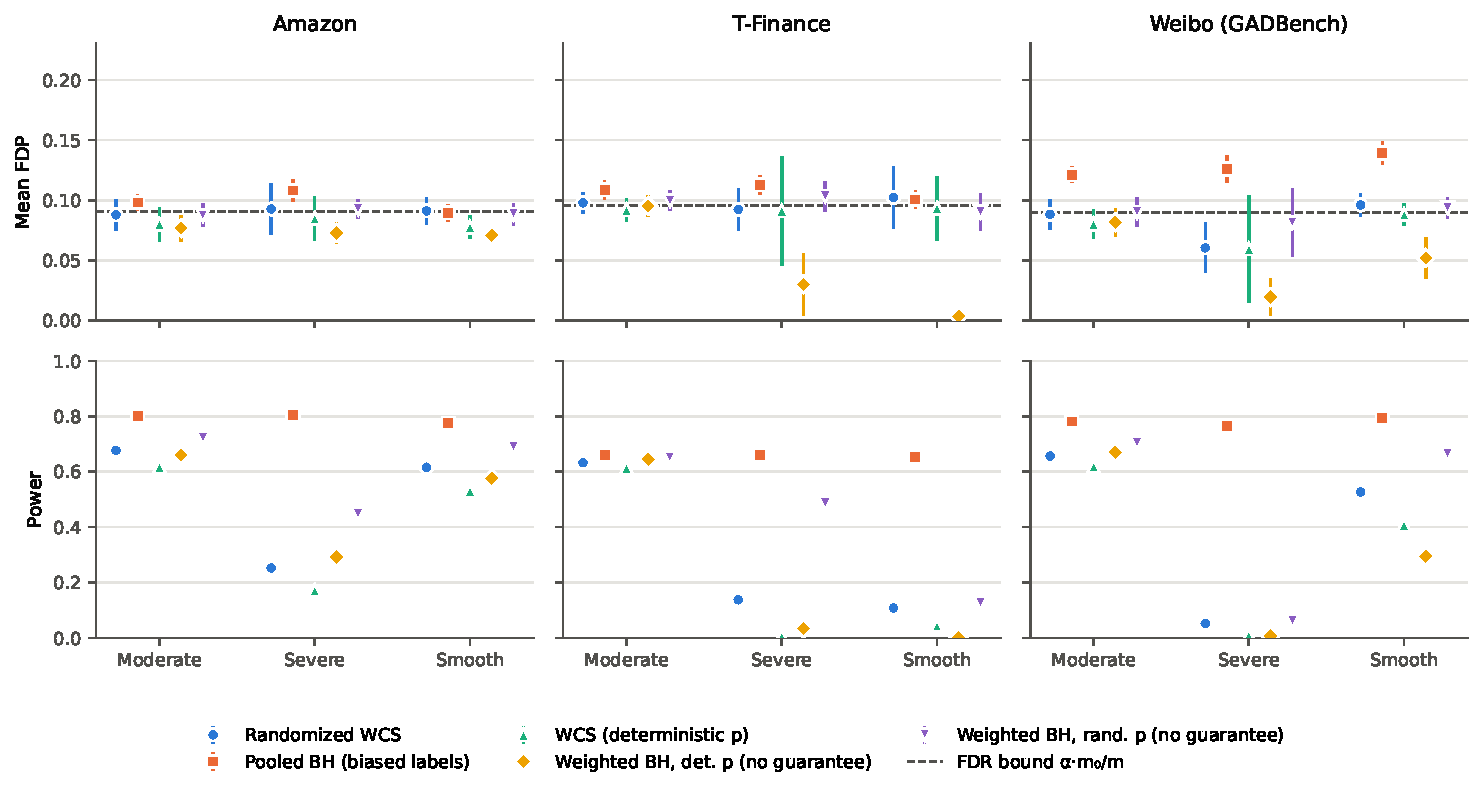
\includegraphics[width=\textwidth]{wcs_endtoend_figure_attributes.pdf}
\caption{Companion to Figure~\ref{fig:endtoend} for the attribute scorer. Same design, averaging and interval conventions.}
\label{fig:endtoendattr}
\end{figure*}

\begin{table*}[t]
\centering\footnotesize\setlength{\tabcolsep}{4pt}
\caption{Resolution diagnostic on the frozen-score acquisition experiments with the 80/20 exposure strata and the graph-feature scorer: Kish effective reference size $(\sum w)^2/\sum w^2$, the median required rejection count $mf/\alpha$ for test anomalies in the sparse stratum (deterministic $p$-values; homogeneous pruning multiplies it by $\xi$), the share of test anomalies in that stratum, and power for WCS with deterministic and randomized $p$-values.}
\label{tab:resolution}\begin{tabular}{llccccc}
\toprule
Graph & Bias & Kish ESS & $mf/\alpha$ & Anomaly share & WCS (det.\ $p$) & Randomized WCS\\
\midrule
Amazon & None & 2638 & 7 & 0.51 & 0.789 & 0.790\\
Amazon & Moderate & 1580 & 37 & 0.51 & 0.758 & 0.773\\
Amazon & Severe & 640 & 146 & 0.51 & 0.160 & 0.331\\
T-Finance & None & 12670 & 7 & 0.88 & 0.791 & 0.791\\
T-Finance & Moderate & 7586 & 35 & 0.88 & 0.773 & 0.780\\
T-Finance & Severe & 3041 & 140 & 0.88 & 0.730 & 0.766\\
Weibo (GADBench) & None & 2543 & 7 & 0.91 & 0.848 & 0.850\\
Weibo (GADBench) & Moderate & 1737 & 37 & 0.91 & 0.790 & 0.813\\
Weibo (GADBench) & Severe & 812 & 148 & 0.91 & 0.197 & 0.345\\
\bottomrule
\end{tabular}

\end{table*}

\begin{table*}[t]
\centering\small
\caption{End-to-end biased acquisition (all methods): mean FDP / power at nominal $0.10$ over ten seeds, five splits and three acquisition draws, with the scorer retrained on the acquired labels. The bound $\alpha m_0/m$ is $0.090$ on Amazon and Weibo and $0.095$ on T-Finance. Weighted BH ($\dagger$) has no guarantee here; the randomized columns share the same auxiliary uniforms, and both WCS columns use homogeneous pruning.}
\label{tab:endtoend}{\footnotesize\setlength{\tabcolsep}{2.5pt}\begin{tabular}{lllccccc}
\toprule
Graph & Scorer & Bias & Pooled BH & W.\ BH, det.\ $p^\dagger$ & W.\ BH, rand.\ $p^\dagger$ & WCS, det.\ $p$ & WCS, rand.\ $p$\\
\midrule
Amazon & Graph & Moderate & 0.108 / 0.815 & 0.080 / 0.700 & 0.087 / 0.739 & 0.082 / 0.672 & 0.087 / 0.708\\
Amazon & Graph & Severe & 0.115 / 0.818 & 0.075 / 0.295 & 0.095 / 0.470 & 0.079 / 0.169 & 0.089 / 0.254\\
Amazon & Graph & Smooth & 0.088 / 0.789 & 0.075 / 0.606 & 0.091 / 0.715 & 0.086 / 0.574 & 0.093 / 0.626\\
Amazon & Attr. & Moderate & 0.098 / 0.803 & 0.077 / 0.661 & 0.087 / 0.722 & 0.080 / 0.618 & 0.088 / 0.677\\
Amazon & Attr. & Severe & 0.108 / 0.806 & 0.073 / 0.292 & 0.093 / 0.447 & 0.085 / 0.172 & 0.093 / 0.253\\
Amazon & Attr. & Smooth & 0.090 / 0.775 & 0.071 / 0.576 & 0.088 / 0.689 & 0.078 / 0.532 & 0.091 / 0.616\\
\midrule
T-Finance & Graph & Moderate & 0.159 / 0.828 & 0.096 / 0.790 & 0.102 / 0.796 & 0.096 / 0.785 & 0.102 / 0.796\\
T-Finance & Graph & Severe & 0.180 / 0.832 & 0.066 / 0.542 & 0.089 / 0.708 & 0.068 / 0.416 & 0.092 / 0.518\\
T-Finance & Graph & Smooth & 0.175 / 0.830 & 0.007 / 0.001 & 0.092 / 0.199 & 0.080 / 0.050 & 0.095 / 0.136\\
T-Finance & Attr. & Moderate & 0.109 / 0.660 & 0.095 / 0.645 & 0.100 / 0.651 & 0.092 / 0.614 & 0.098 / 0.633\\
T-Finance & Attr. & Severe & 0.113 / 0.659 & 0.030 / 0.033 & 0.103 / 0.486 & 0.091 / 0.007 & 0.092 / 0.138\\
T-Finance & Attr. & Smooth & 0.101 / 0.653 & 0.004 / 0.000 & 0.090 / 0.125 & 0.094 / 0.045 & 0.102 / 0.108\\
\midrule
Weibo (GADBench) & Graph & Moderate & 0.158 / 0.943 & 0.081 / 0.783 & 0.090 / 0.829 & 0.080 / 0.754 & 0.091 / 0.792\\
Weibo (GADBench) & Graph & Severe & 0.177 / 0.947 & 0.025 / 0.010 & 0.083 / 0.108 & 0.047 / 0.008 & 0.081 / 0.106\\
Weibo (GADBench) & Graph & Smooth & 0.176 / 0.950 & 0.063 / 0.493 & 0.088 / 0.787 & 0.084 / 0.568 & 0.089 / 0.660\\
Weibo (GADBench) & Attr. & Moderate & 0.121 / 0.782 & 0.082 / 0.671 & 0.090 / 0.705 & 0.080 / 0.619 & 0.088 / 0.657\\
Weibo (GADBench) & Attr. & Severe & 0.126 / 0.766 & 0.020 / 0.007 & 0.081 / 0.061 & 0.060 / 0.009 & 0.061 / 0.052\\
Weibo (GADBench) & Attr. & Smooth & 0.139 / 0.795 & 0.052 / 0.294 & 0.094 / 0.663 & 0.088 / 0.409 & 0.096 / 0.527\\
\bottomrule
\end{tabular}
}
\end{table*}

\clearpage\section{RANDOMIZED WEIGHTED BH AND THE SHARPER BOUND}
\label{app:wbhcounter}

Theorem~\ref{thm:design} gives WCS the bound $\alpha m_0/m$. The example below shows that BH applied to the same randomized weighted $p$-values of Equation~\eqref{eq:randp} need not satisfy that bound under the same design. It does not show a failure of FDR control at the nominal level $\alpha$, which remains open.

\paragraph{A three-node example.}
Take two normal nodes $a$ and $b$ and one anomaly $c$, with scores $s_c<s_a<s_b$, acquisition probabilities $\rho(a)=\rho(c)=0.3$ and $\rho(b)=1$, and weights $w=1/\rho$. One of $a,b$ is chosen uniformly as the null test node, the anomaly is always tested ($m=2$, $m_0=1$), the other normal is acquired with its probability and enters the reference, and $\alpha=0.5$, so the BH thresholds are $0.25$ and $0.5$. If $a$ is tested, the reference is $\{b\}$ and $p_a$ and $p_c$ are independent and uniform on $[3/13,1]$; conditional on $a$ being tested, the expected FDP is $0.35^2/2+0.025\times0.65=0.0775$, since FDP is $1/2$ when both are rejected and $1$ when $a$ alone is. If $b$ is tested and $a$ was acquired (probability $0.3$), then $p_b\le3/13<0.25$ and $p_c\ge0.5$, so $b$ alone is rejected and FDP $=1$. If $b$ is tested and $a$ was not acquired, the reference is empty, $p_b$ and $p_c$ are independent uniforms, and the conditional expected FDP is $0.25$. Hence
\[
\mathrm{FDR}=\tfrac12(0.0775)+\tfrac12\{0.3+0.7(0.25)\}=\tfrac{221}{800}=0.27625>\alpha m_0/m=0.25 .
\]
For randomized WCS with homogeneous pruning on the same design, integrating exactly over the randomized $p$-values and the pruning coin gives conditional expected FDPs $0.020625$ when $a$ is tested, and $1$ and $0.1875$ when $b$ is tested with and without a reference, so its FDR is $723/3200=0.2259375$, below the bound as Theorem~\ref{thm:design} requires; a Monte Carlo estimate ($400{,}000$ draws) agrees. Both procedures are below the nominal $0.5$.

\paragraph{Scope of the search.}
The example came from a protocol fixed before execution: exact evaluation of $20{,}000$ random finite designs within the assumptions of Theorem~\ref{thm:design} (two to six normals, at most four test nodes, $\rho$ on a grid from $0.01$ to $1$, $\alpha\in\{0.05,0.1,0.2,0.3,0.5\}$), followed by local search. Exact values were cross-checked against an independent implementation and Monte Carlo. Randomized weighted BH exceeded $\alpha m_0/m$ in $618$ of the $20{,}000$ randomly generated designs (a descriptive count that depends on how designs were generated, not a failure rate), at every $\alpha$ tested, by at most $0.0009$ at $\alpha\le0.1$ and $0.026$ at $\alpha=0.5$; no design exceeded the nominal $\alpha$, which leaves nominal validity unresolved rather than established, deterministic weighted BH never exceeded $\alpha m_0/m$, and every exceedance required an anomaly in the test set. A separate five-node design with the largest excess (three normals and two anomalies, excess $0.027$), not the three-node example above, was replicated $2$ to $25$ times with the same probabilities and score blocks, and under that replication scheme the excess was no longer detectable (Monte Carlo, $20{,}000$ draws per size). This does not rule out counterexamples in larger populations. The example separates the sharper guarantees of the two procedures; it is not evidence about the benchmark graphs, where no clear violation was detected (Section~\ref{sec:results}).


\section{UNIFORM ACQUISITION AT THE SAME BUDGET}
\label{app:uniform}
For each biased design and each graph and training seed, the uniform design acquires every non-test deployment node independently with probability $\rho_u$, the mean of the prescribed $\rho(v)$ over the whole deployment population, fixed before test nodes are assigned. A rate computed from the realized non-test nodes of each split would make a node's acquisition probability depend on which nodes are tested, which Theorem~\ref{thm:design} does not allow; a first version of this experiment made that error and was stopped and replaced before any result was summarized. Because test counts are stratified by class and rounded, the expected per-split label counts under the two designs are not exactly equal; their largest difference is $2.2$ labels. Acquisition reuses the same uniform draws, training coins, scorer seeds and auxiliary uniforms as the biased run. Under uniform acquisition the weights are constant, so randomized WCS is covered by Theorem~\ref{thm:design}, and pooled BH on the acquired reference is also valid; its power is within $0.007$ of randomized WCS in every cell. Table~\ref{tab:uniform} gives all 18 cells; intervals are seed-clustered 95\% $t$ intervals for the paired difference in power.

\begin{table*}[t]
\centering\footnotesize
\caption{Randomized WCS under each biased design and under uniform acquisition at approximately the same expected label budget: mean power, paired difference (uniform minus biased) with seed-clustered 95\% interval, and mean FDP under uniform acquisition. Bounds $\alpha m_0/m$ are $0.090$ on Amazon and Weibo and $0.095$ on T-Finance.}
\label{tab:uniform}\begin{tabular}{lllcccc}
\toprule
Graph & Scorer & Bias & Biased power & Uniform power & Difference [95\% CI] & Uniform FDP\\
\midrule
Amazon & Graph & Moderate & 0.708 & 0.802 & 0.094 [0.054, 0.134] & 0.091\\
Amazon & Graph & Severe & 0.254 & 0.798 & 0.544 [0.508, 0.581] & 0.087\\
Amazon & Graph & Smooth & 0.626 & 0.788 & 0.163 [0.125, 0.200] & 0.089\\
Amazon & Attr. & Moderate & 0.677 & 0.790 & 0.113 [0.046, 0.181] & 0.090\\
Amazon & Attr. & Severe & 0.253 & 0.783 & 0.531 [0.493, 0.568] & 0.089\\
Amazon & Attr. & Smooth & 0.616 & 0.768 & 0.151 [0.118, 0.185] & 0.094\\
\midrule
T-Finance & Graph & Moderate & 0.796 & 0.808 & 0.012 [0.008, 0.016] & 0.101\\
T-Finance & Graph & Severe & 0.518 & 0.805 & 0.286 [0.193, 0.379] & 0.099\\
T-Finance & Graph & Smooth & 0.136 & 0.805 & 0.668 [0.635, 0.701] & 0.101\\
T-Finance & Attr. & Moderate & 0.633 & 0.664 & 0.032 [0.008, 0.055] & 0.100\\
T-Finance & Attr. & Severe & 0.138 & 0.664 & 0.526 [0.506, 0.546] & 0.101\\
T-Finance & Attr. & Smooth & 0.108 & 0.659 & 0.551 [0.522, 0.581] & 0.097\\
\midrule
Weibo (GADBench) & Graph & Moderate & 0.792 & 0.905 & 0.113 [0.078, 0.149] & 0.093\\
Weibo (GADBench) & Graph & Severe & 0.106 & 0.904 & 0.799 [0.772, 0.826] & 0.094\\
Weibo (GADBench) & Graph & Smooth & 0.660 & 0.907 & 0.248 [0.182, 0.313] & 0.095\\
Weibo (GADBench) & Attr. & Moderate & 0.657 & 0.773 & 0.116 [0.075, 0.157] & 0.093\\
Weibo (GADBench) & Attr. & Severe & 0.052 & 0.773 & 0.720 [0.694, 0.747] & 0.094\\
Weibo (GADBench) & Attr. & Smooth & 0.527 & 0.785 & 0.258 [0.207, 0.309] & 0.096\\
\bottomrule
\end{tabular}

\end{table*}

\clearpage\section{EXACT CONDITIONAL RANK AUDIT}
\label{app:rankaudit}
Condition on the graph, scores, test set, and an eligible normal reference pool $\mathcal P$ of size $M$. Draw $n\le M$ calibration nodes uniformly without replacement. For a fixed test node, let $K_v=|\{u\in\mathcal P:s(u)\ge s(v)\}|$. Then
\begin{equation}
(n+1)p(v)-1\sim\operatorname{Hypergeom}(M,K_v,n).
\label{eq:hypergeom}
\end{equation}
Writing $H_{M,K,n}$ for this CDF, the expected fraction of null p-values at or below $t$ is
\begin{equation}
\frac{1}{|\testset_0|}\sum_{v\in\testset_0}H_{M,K_v,n}\bigl(\lfloor t(n+1)\rfloor-1\bigr).
\label{eq:exacttail}
\end{equation}
This standard sampling identity permits arbitrary graph dependence and ties: the scores are conditioned on. Changing the reference pool changes its exceedance counts even when $n$ is held fixed. The diagnostic requires labeled development data and evaluates fixed thresholds; it is not an FDR bound at BH's adaptive threshold.

On the untrimmed DOMINANT scores, Equation~\eqref{eq:exacttail} gives expected null fractions at or below $0.01$ of $0.536$ versus $0.00545$ for filtered and random Amazon calibration, and $0.243$ versus $0.01015$ on Tolokers. Filtered GAE and Isolation Forest fractions remain below $0.01$. A separate five-seed Weibo GAE audit gives $0.0233$ versus $0.0095$ without trimming, but filtered mean FDP is only $0.041$ with power $0.004$. The filtered rule averages only 3.7 discoveries per run there, so the crossing of Equation~\eqref{eq:crossing} is rarely reached. A detectable rank shift need not produce many false discoveries. Appendix~\ref{app:fresh} compares the exact calculation with repeated calibration draws.

\section{FRESH GRAPH VALIDATION}
\label{app:fresh}
\begin{table*}[t]
\centering\small
\caption{Complete fresh conditional graph audit, including positive-exposure and larger-random calibration. Each cell averages 200 calibration draws, then reports mean and SD across five score/test realizations. The positive-exposure pool is the binding size constraint in these runs, making its matched calibration draw deterministic once the test set is fixed.}
\label{tab:audit}\begin{tabular}{llrrrr}\toprule Trim & Rule & FDP & Power & Discoveries & $a(0.01)$\\\midrule
0\% & Filtered & $0.041\pm0.033$ & $0.004\pm0.004$ & $3.7\pm3.4$ & 0.0233 \\
0\% & Random & $0.000\pm0.000$ & $0.000\pm0.000$ & $0.0\pm0.0$ & 0.0095 \\
0\% & Positive exposure & $0.000\pm0.000$ & $0.000\pm0.000$ & $0.0\pm0.0$ & 0.0047 \\
0\% & Larger random & $0.000\pm0.000$ & $0.000\pm0.000$ & $0.0\pm0.0$ & 0.0098 \\
1\% & Filtered & $0.249\pm0.108$ & $0.053\pm0.015$ & $27.4\pm10.1$ & 0.0192 \\
1\% & Random & $0.090\pm0.075$ & $0.018\pm0.010$ & $7.8\pm5.0$ & 0.0103 \\
1\% & Positive exposure & $0.000\pm0.000$ & $0.000\pm0.000$ & $0.0\pm0.0$ & 0.0043 \\
1\% & Larger random & $0.130\pm0.080$ & $0.036\pm0.003$ & $14.6\pm2.9$ & 0.0106 \\
5\% & Filtered & $0.084\pm0.037$ & $0.233\pm0.004$ & $88.7\pm4.9$ & 0.0106 \\
5\% & Random & $0.060\pm0.029$ & $0.228\pm0.003$ & $84.3\pm3.5$ & 0.0082 \\
5\% & Positive exposure & $0.031\pm0.029$ & $0.225\pm0.004$ & $80.8\pm3.3$ & 0.0050 \\
5\% & Larger random & $0.065\pm0.036$ & $0.227\pm0.003$ & $84.5\pm3.7$ & 0.0088 \\
\bottomrule\end{tabular}

\end{table*}
The fresh Weibo experiment uses the public PyGOD dataset, with 8,405 nodes, 377,271 edges after conversion to an undirected graph, 400 feature columns, and 347 anomalous labels. The official distributed \texttt{weibo.pt} file contains 8,058 zeros and 347 ones, whereas the repository's descriptive table lists 868 outliers. A fresh download on September 23, 2026 was byte-identical to our cached raw file; we use its actual labels without recoding them to match the table~\citep{pygoddata}. The source-file checksum and label counts are retained in the supplement. We used Python 3.14.2, PyTorch 2.13.0+cpu, PyTorch Geometric 2.8.0, PyGOD 1.1.0, and four CPU threads. Five 100-epoch GAE runs took approximately 23.5 minutes in total. Feature, label, and edge hashes are recorded with the cached scores. The same model settings and graph standardization are used as in the main experiment; the runtime is reported separately rather than assumed identical to the archived GPU environment.

For the conditional audit, each seed/trimming combination has one fixed test set drawn from its eligible normal pool, together with every anomaly. For every rule we make 200 calibration draws, using master seed 20260914 and separate streams by training seed, trimming index, and repetition. There are 12,000 method evaluations across five seeds, three trimming levels, and four rules. Methods share random streams within a repetition, so these are paired evaluations rather than 12,000 independent graph replications. Each per-realization Monte Carlo SE is calculated across calibration draws. The SD in Table~\ref{tab:audit} is instead calculated across the five score/test realizations after averaging those draws. The positive-exposure rule restricts calibration to normal nodes with at least one anomalous neighbor. At thresholds $0.01$ and $0.05$, five seeds, three trimming levels, and four rules give 120 exact-versus-Monte-Carlo tail checks. The maximum absolute discrepancy is $2.9232$ Monte Carlo SEs; all individual checks are supplied in the reproducibility archive.

In the exact audit, a fixed test score defines $K_v$ successes among $M$ eligible calibration nodes. Counting size-$n$ calibration subsets with exactly $k$ successes gives probability $\binom{K_v}{k}\binom{M-K_v}{n-k}/\binom{M}{n}$. Summing these probabilities through $\lfloor t(n+1)\rfloor-1$ proves Equation~\eqref{eq:exacttail} by linearity of expectation over null test nodes. The formula includes ties through the non-strict score comparison. It makes no independence claim about the test-node indicators, and cannot be substituted into BH at its random threshold to obtain an FDR bound.

An additional audit independently reconstructs all 600 primary learned-detector conditions (two graphs, three detectors, ten seeds, five splits, and two reference rules) at $b=1000$. For each condition, 500 fresh calibration draws estimate the null fraction below $0.01$, using master seed 20260921. The maximum absolute difference from Equation~\eqref{eq:exacttail} is $0.000721$. All 300 nonconstant conditions agree within $2.98$ Monte Carlo SEs; the other 300 conditions select the entire eligible filtered pool and agree exactly. SEs are computed across calibration draws, not across nodes. The code and all outcomes are supplied as \texttt{audit\_primary\_ranks.py} and \texttt{primary\_rank\_validation.csv}.

\section{INDEPENDENT GRAPH DETAILS}
\label{app:indgraphs}
\begin{figure*}[t]
\centering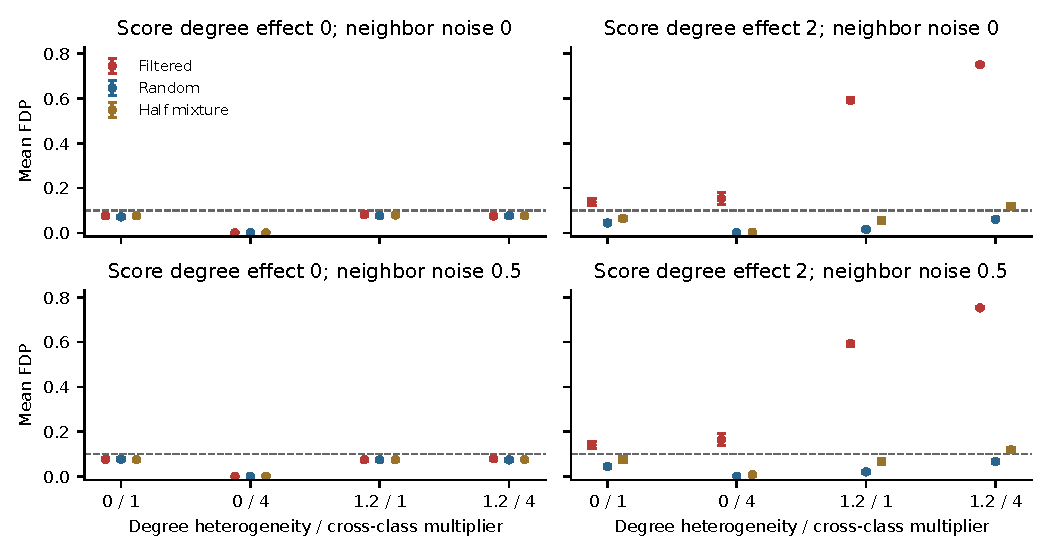
\includegraphics[width=\textwidth]{independent_graphs.pdf}
\caption{Independent graph experiment: mean FDP across 500 graphs per graph-parameter cell, with $1.96$ Monte Carlo SE bars. Each graph is reused across four paired score conditions. Dashed lines mark $0.10$. Selection has its largest effect when heterogeneous degree enters the score; a half-mixture reduces inflation but does not meet the target in every cell. Complete FDP--power results, including partial-label and all-null controls, appear in Table~\ref{tab:indfull}.}
\label{fig:indgraphs}
\end{figure*}
\begin{table*}[t]
\centering\scriptsize
\caption{All independent graph conditions: mean FDP / power over 500 graph draws per row. Four score conditions share each non-null graph. Partial-label comparisons reveal 25\% of non-test labels. Power is recorded as zero by convention in the all-null control, where no alternatives exist.}
\label{tab:indfull}\begin{tabular}{rrrrrrrrrr}\toprule
All-null & $\sigma$ & $c$ & $\theta$ & $\eta$ & Filter & Random & Mixture & Partial & Partial random\\\midrule
0 & 0 & 1 & 0 & 0 & 0.077 / 0.911 & 0.072 / 0.909 & 0.076 / 0.910 & 0.059 / 0.883 & 0.060 / 0.888 \\
0 & 0 & 1 & 0 & 0.5 & 0.077 / 0.916 & 0.077 / 0.911 & 0.076 / 0.913 & 0.068 / 0.883 & 0.069 / 0.892 \\
0 & 0 & 1 & 2 & 0 & 0.139 / 0.265 & 0.045 / 0.101 & 0.065 / 0.136 & 0.041 / 0.086 & 0.031 / 0.066 \\
0 & 0 & 1 & 2 & 0.5 & 0.140 / 0.268 & 0.045 / 0.098 & 0.077 / 0.163 & 0.035 / 0.070 & 0.022 / 0.048 \\
0 & 0 & 4 & 0 & 0 & 0.000 / 0.000 & 0.001 / 0.002 & 0.000 / 0.000 & 0.065 / 0.671 & 0.063 / 0.654 \\
0 & 0 & 4 & 0 & 0.5 & 0.000 / 0.000 & 0.001 / 0.002 & 0.001 / 0.002 & 0.062 / 0.695 & 0.065 / 0.707 \\
0 & 0 & 4 & 2 & 0 & 0.154 / 0.222 & 0.001 / 0.002 & 0.004 / 0.006 & 0.097 / 0.916 & 0.068 / 0.894 \\
0 & 0 & 4 & 2 & 0.5 & 0.165 / 0.232 & 0.001 / 0.002 & 0.008 / 0.012 & 0.097 / 0.901 & 0.067 / 0.889 \\
0 & 1.2 & 1 & 0 & 0 & 0.081 / 0.911 & 0.077 / 0.909 & 0.080 / 0.916 & 0.071 / 0.899 & 0.067 / 0.890 \\
0 & 1.2 & 1 & 0 & 0.5 & 0.076 / 0.914 & 0.075 / 0.910 & 0.076 / 0.919 & 0.063 / 0.891 & 0.060 / 0.885 \\
0 & 1.2 & 1 & 2 & 0 & 0.592 / 0.704 & 0.016 / 0.024 & 0.056 / 0.068 & 0.141 / 0.164 & 0.008 / 0.011 \\
0 & 1.2 & 1 & 2 & 0.5 & 0.593 / 0.711 & 0.021 / 0.027 & 0.067 / 0.087 & 0.138 / 0.174 & 0.012 / 0.018 \\
0 & 1.2 & 4 & 0 & 0 & 0.076 / 0.908 & 0.076 / 0.904 & 0.077 / 0.896 & 0.061 / 0.797 & 0.060 / 0.800 \\
0 & 1.2 & 4 & 0 & 0.5 & 0.080 / 0.921 & 0.075 / 0.916 & 0.076 / 0.916 & 0.065 / 0.841 & 0.066 / 0.839 \\
0 & 1.2 & 4 & 2 & 0 & 0.751 / 0.979 & 0.061 / 0.288 & 0.119 / 0.416 & 0.373 / 0.764 & 0.036 / 0.134 \\
0 & 1.2 & 4 & 2 & 0.5 & 0.753 / 0.979 & 0.067 / 0.336 & 0.120 / 0.451 & 0.370 / 0.771 & 0.038 / 0.147 \\
1 & 1.2 & 1 & 2 & 0.5 & 0.000 / 0.000 & 0.004 / 0.000 & 0.000 / 0.000 & 0.000 / 0.000 & 0.000 / 0.000 \\
\bottomrule\end{tabular}

\end{table*}
For each graph, choose 120 anomalous nodes uniformly among 1,200. Generate independent $Z_i\sim N(0,1)$, set $a_i=\exp(\sigma Z_i-\sigma^2/2)$, and divide $a_i$ by its sample mean. For $i<j$, let $b_{ij}=c$ for different labels and 1 otherwise, and let $\bar b$ be the mean over unordered pairs. Edges are independent conditional on propensities and labels, with probability $\min\{0.9,12a_ia_jb_{ij}/(1199\bar b)\}$. The code records clipping fractions and realized edge counts. This normalization targets comparable density approximately, rather than conditioning all graphs on an identical edge count.

Let $z_i$ be new independent standard normals and $d_i$ the realized degree. Write $h_i=\sum_j A_{ij}z_j/\sqrt{d_i\vee1}$. Noise is
\[
\varepsilon_i=\frac{\sqrt{1-\eta}\,z_i+\sqrt{\eta}\,h_i}
{\sqrt{1-\eta+\eta\ind\{d_i>0\}}}.
\]
This preserves unit marginal variance conditional on the graph, including isolated nodes, while permitting shared-neighbor dependence when $\eta>0$. Standardized $\log(1+d_i)$ supplies $L_i$. The same graph, test set, and calibration assignments are reused across the four $(\theta,\eta)$ conditions. The all-null control uses $(\sigma,c,\theta,\eta)=(1.2,1,2,0.5)$ and zero anomalies. Master seed 20260920, graph index, and graph parameters determine separate NumPy seed streams. There are 2,500 unique graphs and 42,500 method evaluations; full Monte Carlo SEs and reference sizes are in the supplied CSVs.

\section{COMPLETE SCORE SIMULATION}
\label{app:simulation}
\paragraph{A covariate mechanism.}
Suppose calibration selection is described by a covariate $W$ and an indicator $A$. A covariate shift translates into a score shift if the conditional score law is the same in selected and target populations, $S\perp A\mid W$, and $S\mid W=w$ is stochastically nondecreasing in $w$. Under these assumptions, a stochastically smaller selected $W$ gives a stochastically smaller score (Appendix~\ref{app:proofs}). The common conditional-law assumption is essential: a shift in degree alone does not establish it. For an exposure filter, zero-exposure calibration has a degenerate exposure distribution. Degree can shift as a secondary consequence, but a correlation or a plot of bin medians cannot establish the required conditional stochastic order.

\paragraph{What weighting requires.}
In an independent covariate-shift model, let $w(W)=dP_0^W/dP_C^W$ be the target-to-calibration density ratio. With a common conditional score law, a conservative weighted rank takes the form
\begin{equation}
 p_w(v)=\frac{w(W_v)+\sum_{i=1}^n w(W_i)\ind\{S_i\ge s(v)\}}
 {w(W_v)+\sum_{i=1}^n w(W_i)}.
 \label{eq:weighted}
\end{equation}
The \emph{same} ratio function applies to calibration and test points~\citep{tibshirani2019conformal}. If the target is the full normal population and $q(w)=\Prb(A=1\mid W=w)$, then $w(w)\propto1/q(w)$. A common multiplicative constant cancels only when applied to all weights, including the test point. If the target is instead the unselected complement, the ratio is proportional to $(1-q)/q$.

Equation~\eqref{eq:weighted} requires target support to be covered by calibration support and the conditional-law assumptions to hold. A fitted degree propensity need not repair selection on other features of a neighborhood. Even correct marginal weighted p-values require a separate dependence argument before asserting BH FDR control; Theorem~\ref{thm:design} supplies that argument for the acquisition design of Section~\ref{sec:method}, and the simulations below compare weighted BH with the hypothesis-conditional WCS procedure of \citet{jin2026weighted} under independent sampling.

\subsection{Independent score and weighting comparisons}
We use a two-stratum score model to vary score sensitivity independently of selection strength. A normal target has $W\sim\operatorname{Bernoulli}(1/2)$ and $S=\theta W+Z$, where $Z\sim N(0,1)$. An anomalous target has the same covariate law and score $S=\theta W+Z+3$. Each repetition has $n=200$ normal calibration scores and $m=400$ test scores, of which 360 are normal. Calibration and test observations are independent. Within each repetition, methods share random numbers to reduce comparison noise.

Selection retains stratum $W=0$ with probability one and stratum $W=1$ with probability $q\in\{1,0.25,0.05,0\}$. Conditional on selection, $\Prb_C(W=1)=q/(1+q)$. We consider $\theta\in\{0,2\}$. For $q>0$, correct weights are $1/q(W)$ at both calibration and test points. We also evaluate the fixed test-weight heuristic, using the same calibration weights but test weight one. At $q=0$, no density-ratio correction is available for target stratum $W=1$, and we omit weighted results. Zero feature overlap does not by itself destroy rank validity when the score is independent of that feature, as the $\theta=0$ control illustrates. Each configuration uses 2,000 independent repetitions; these experiments validate the independent score model, not graph dependence.

\paragraph{Selection and score sensitivity interact.}
When $\theta=0$, ordinary filtered and random calibration have identical paired score vectors: mean FDP is $0.0648$ and power $0.5267$ for every $q$. When $\theta=2$, mean FDP rises from $0.0533$ at $q=1$ to $0.1666$, $0.5628$, and $0.7318$ as $q$ decreases (Figure~\ref{fig:simulation}). The probability of a null p-value below $0.05$ rises from $0.0497$ to $0.3386$. Here the covariate and conditional score assumptions are controlled by construction, so the experiment directly illustrates Proposition~\ref{prop:order}.

\paragraph{The test weight changes the conclusion.}
At $\theta=2,q=0.05$, the correct formula yields mean FDP $0.0067$ and power $0.0557$, while fixing the test weight at one yields $0.3375$ and $0.6190$. The fixed-weight heuristic also gives mean FDP $0.1421$ when $\theta=0,q=0.05$, despite no selection-induced score shift. The test-point mass changes attainable p-values and can strongly affect the BH rejection set. These results support correcting the formula, while showing that marginal validity can come with poor power in a finite reference sample.

\paragraph{Contamination is a separate intervention.}
We additionally replace each unfiltered calibration observation with an independently generated anomalous observation with probability $0.05$ or $0.10$, using the same anomaly score law as above. No test observation is reused. Mean FDP is at most $0.0010$ in these configurations, but power is at most $0.0079$; the 10\% conditions make no discoveries. This is a narrow conservative example, not evidence that arbitrary contamination is harmless. At fixed $n$, increasing calibration scores can only increase p-values, but the resolution floor remains $1/(n+1)$. A shrinking rejection set need not have a smaller FDP if it loses true discoveries disproportionately. Appendix~\ref{app:proofs} gives an explicit attainable counterexample.

\begin{figure*}[t]
\centering
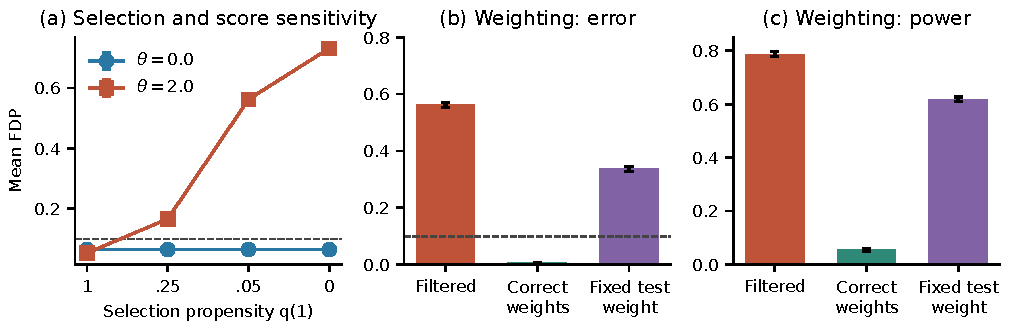
\includegraphics[width=\textwidth]{selection_validation.pdf}
\caption{Independent score experiment, 2,000 repetitions per configuration. (a) Filtering affects ordinary ranks when scores depend on the selected covariate ($\theta=2$); with $\theta=0$ the score vectors are identical under the paired construction. (b,c) At $\theta=2$ and $q(1)=0.05$, correct test-point weighting reduces mean FDP but also power. Dashed lines mark $\alpha=0.10$; error bars are $1.96$ Monte Carlo standard errors, not graph-level uncertainty intervals.}
\label{fig:simulation}
\end{figure*}
\begin{table*}[t]
\centering\small
\caption{All independent simulation configurations. FDP uncertainty is Monte Carlo SE across 2,000 repetitions. Power and null-tail entries are means. $\epsilon$ is the contamination probability; no test observation is reused for calibration. Correct weights are omitted at $q=0$ because the target contains a stratum absent from calibration.}
\begin{tabular}{rrrlrrr}\toprule $\theta$ & $q(1)$ & $\epsilon$ & Method & FDP $\pm$ MCSE & Power & $\Prb_0(p\le.05)$\\\midrule
0.0 & 1.0 & 0.0 & Random & 0.0648 $\pm$ 0.0017 & 0.5267 & 0.0500 \\
0.0 & 0.25 & 0.0 & Filtered & 0.0648 $\pm$ 0.0017 & 0.5267 & 0.0500 \\
0.0 & 0.25 & 0.0 & Correct weights & 0.0439 $\pm$ 0.0016 & 0.1904 & 0.0465 \\
0.0 & 0.25 & 0.0 & Fixed test weight & 0.1042 $\pm$ 0.0019 & 0.6841 & 0.0510 \\
0.0 & 0.05 & 0.0 & Filtered & 0.0648 $\pm$ 0.0017 & 0.5267 & 0.0500 \\
0.0 & 0.05 & 0.0 & Correct weights & 0.0601 $\pm$ 0.0019 & 0.2414 & 0.0340 \\
0.0 & 0.05 & 0.0 & Fixed test weight & 0.1421 $\pm$ 0.0022 & 0.7459 & 0.0607 \\
0.0 & 0.0 & 0.0 & Filtered & 0.0648 $\pm$ 0.0017 & 0.5267 & 0.0500 \\
0.0 & 1.0 & 0.05 & Contaminated & 0.0003 $\pm$ 0.0001 & 0.0079 & 0.0132 \\
0.0 & 1.0 & 0.1 & Contaminated & 0.0000 $\pm$ 0.0000 & 0.0000 & 0.0020 \\
2.0 & 1.0 & 0.0 & Random & 0.0533 $\pm$ 0.0020 & 0.1762 & 0.0497 \\
2.0 & 0.25 & 0.0 & Filtered & 0.1666 $\pm$ 0.0038 & 0.3732 & 0.1183 \\
2.0 & 0.25 & 0.0 & Correct weights & 0.0049 $\pm$ 0.0011 & 0.0090 & 0.0443 \\
2.0 & 0.25 & 0.0 & Fixed test weight & 0.1524 $\pm$ 0.0028 & 0.4361 & 0.0514 \\
2.0 & 0.05 & 0.0 & Filtered & 0.5628 $\pm$ 0.0043 & 0.7867 & 0.2683 \\
2.0 & 0.05 & 0.0 & Correct weights & 0.0067 $\pm$ 0.0006 & 0.0557 & 0.0197 \\
2.0 & 0.05 & 0.0 & Fixed test weight & 0.3375 $\pm$ 0.0042 & 0.6190 & 0.0614 \\
2.0 & 0.0 & 0.0 & Filtered & 0.7318 $\pm$ 0.0011 & 0.9329 & 0.3386 \\
2.0 & 1.0 & 0.05 & Contaminated & 0.0010 $\pm$ 0.0003 & 0.0038 & 0.0231 \\
2.0 & 1.0 & 0.1 & Contaminated & 0.0000 $\pm$ 0.0000 & 0.0000 & 0.0078 \\
\bottomrule\end{tabular}

\end{table*}
The master seed is 20260913. Repetition $b$ uses NumPy's \texttt{SeedSequence([20260913,b])}; repetitions are independent, while arms within a repetition use common random numbers. Normal and anomalous test residuals are independent of calibration residuals. Contaminant residuals, covariates, and replacement indicators are drawn independently of test data. Calibration and test index sets are disjoint by construction.

The weighted rank is checked against direct summation, including tied scores, and against ordinary conformal ranks when every weight is one. Multiplying all calibration and test weights by the same positive constant leaves the result unchanged. Validation also checks the deterministic rank floor and an attainable FDP counterexample. Independently integrating the binomial-mixture law in Equation~\eqref{eq:binomial} gives theoretical null-tail probabilities at $0.05$ and $0.10$ for each ordinary-rank configuration; the accompanying output reports all 16 comparisons with Monte Carlo estimates. Complete per-repetition results are retained, allowing paired contrasts or alternative uncertainty summaries without rerunning the simulation. The error bars in Figure~\ref{fig:simulation} quantify Monte Carlo precision for this specified model only.

\section{WEIGHTED CONFORMAL SELECTION UNDER INDEPENDENT SAMPLING}
\label{app:wcs}
\begin{table*}[t]
\centering\small
\caption{Complete WCS comparison under independent sampling. FDP entries give mean (Monte Carlo SE) over 2,000 independent repetitions; power entries are means. At $q=1$, ordinary and weighted BH and both WCS variants coincide in this simulation. Zero-discovery runs are retained.}
\begin{tabular}{rrlrr}\toprule
$\theta$ & $q$ & Method & FDP (MCSE) & Power\\\midrule
0 & 1 & Ordinary BH & $0.0693\;( 0.0017)$ & 0.5415 \\
0 & 1 & Weighted BH & $0.0693\;( 0.0017)$ & 0.5415 \\
0 & 1 & WCS deterministic & $0.0693\;( 0.0017)$ & 0.5415 \\
0 & 1 & WCS homogeneous & $0.0693\;( 0.0017)$ & 0.5415 \\
0 & 1 & Weighted BY & $0.0000\;( 0.0000)$ & 0.0000 \\
0 & 0.25 & Ordinary BH & $0.0693\;( 0.0017)$ & 0.5415 \\
0 & 0.25 & Weighted BH & $0.0477\;( 0.0017)$ & 0.2039 \\
0 & 0.25 & WCS deterministic & $0.0001\;( 0.0001)$ & 0.0005 \\
0 & 0.25 & WCS homogeneous & $0.0561\;( 0.0021)$ & 0.1814 \\
0 & 0.25 & Weighted BY & $0.0000\;( 0.0000)$ & 0.0000 \\
0 & 0.05 & Ordinary BH & $0.0693\;( 0.0017)$ & 0.5415 \\
0 & 0.05 & Weighted BH & $0.0621\;( 0.0019)$ & 0.2513 \\
0 & 0.05 & WCS deterministic & $0.0000\;( 0.0000)$ & 0.0000 \\
0 & 0.05 & WCS homogeneous & $0.0744\;( 0.0025)$ & 0.1949 \\
0 & 0.05 & Weighted BY & $0.0000\;( 0.0000)$ & 0.0000 \\
2 & 1 & Ordinary BH & $0.0535\;( 0.0020)$ & 0.1700 \\
2 & 1 & Weighted BH & $0.0535\;( 0.0020)$ & 0.1700 \\
2 & 1 & WCS deterministic & $0.0535\;( 0.0020)$ & 0.1700 \\
2 & 1 & WCS homogeneous & $0.0535\;( 0.0020)$ & 0.1700 \\
2 & 1 & Weighted BY & $0.0000\;( 0.0000)$ & 0.0000 \\
2 & 0.25 & Ordinary BH & $0.1706\;( 0.0038)$ & 0.3822 \\
2 & 0.25 & Weighted BH & $0.0049\;( 0.0011)$ & 0.0079 \\
2 & 0.25 & WCS deterministic & $0.0036\;( 0.0009)$ & 0.0059 \\
2 & 0.25 & WCS homogeneous & $0.0056\;( 0.0012)$ & 0.0202 \\
2 & 0.25 & Weighted BY & $0.0000\;( 0.0000)$ & 0.0000 \\
2 & 0.05 & Ordinary BH & $0.5733\;( 0.0042)$ & 0.7928 \\
2 & 0.05 & Weighted BH & $0.0071\;( 0.0007)$ & 0.0610 \\
2 & 0.05 & WCS deterministic & $0.0000\;( 0.0000)$ & 0.0000 \\
2 & 0.05 & WCS homogeneous & $0.0037\;( 0.0005)$ & 0.0328 \\
2 & 0.05 & Weighted BY & $0.0000\;( 0.0000)$ & 0.0000 \\
\bottomrule\end{tabular}

\end{table*}
This experiment uses master seed 20260916, 200 independent calibration observations, 400 test observations including 360 nulls, and the same two-stratum score model as Appendix~\ref{app:simulation}. Values $q=1,0.25,0.05$ ensure positive support. The $q=1$ cell is the unselected ordinary-BH reference. Methods share data within a repetition; repetitions are independent. Homogeneous WCS pruning uses a separate uniform draw shared across its selected hypotheses. BY uses nominal level $0.10/\sum_{j=1}^{400}1/j$ on the weighted p-values~\citep{benjamini2001control}. At $\theta=2,q=0.05$, ordinary BH has mean FDP $0.573$ and power $0.793$; weighted BH gives $0.0071$ and $0.0610$; homogeneous WCS gives $0.0037$ and $0.0328$; deterministic WCS and weighted BY make no discoveries. With only 200 reference observations the resolution floor of Proposition~\ref{prop:wresolution} binds, which is why the graph experiments with thousands of reference nodes behave differently.

Our implementation follows the nonrandomized ranks and hypothesis-conditional Algorithm 2 in the versioned source~\citep{jin2023algorithm}. It was checked against a literal equation implementation on 80 random cases, including weight rescaling and test permutation, and against six constant-weight cases of the authors' reference implementation. The inspected reference file used a different test-weight index in an auxiliary numerator and randomized ranks; variable-weight agreement with that file is therefore not claimed. The source hash and precise discrepancy are recorded in \texttt{wcs\_validation.json}. This is implementation provenance, not an empirical comparison against running the authors' variable-weight software.

\clearpage\section{OBSERVED-EXPOSURE REMOVAL SENSITIVITY}
\label{app:dose}
This exploratory follow-up was specified after external feedback on the manuscript. The Amazon/Tolokers grid was fixed before its outcomes were inspected; the Weibo extension was specified after those two-graph results, before fitting its supervised models. We retain both scorers and every condition. Weibo uses the official file described in Appendix~\ref{app:fresh}, the same fixed classifier settings as Appendix~\ref{app:supervised}, and a uniform 10\% training panel (840 labels), with ten training seeds and five test splits per seed. Its graph features use the same unweighted neighbor means and log degree. Training runs use one CPU thread; no Weibo outcome was used to tune model settings.

\begin{table}[ht]\centering\small
\caption{Ranking quality on all nontraining nodes: mean $\pm$ SD across ten training seeds. Average precision is reported alongside AUROC because discovery uses the upper score tail.}
\begin{tabular}{llrr}\toprule Graph & Score & AUROC & Average precision\\\midrule
Amazon & Attributes & $0.969\pm0.002$ & $0.895\pm0.007$ \\
Amazon & Attributes + graph & $0.971\pm0.005$ & $0.898\pm0.009$ \\
Tolokers & Attributes & $0.706\pm0.009$ & $0.345\pm0.012$ \\
Tolokers & Attributes + graph & $0.790\pm0.006$ & $0.472\pm0.011$ \\
Weibo & Attributes & $0.929\pm0.006$ & $0.292\pm0.014$ \\
Weibo & Attributes + graph & $0.948\pm0.003$ & $0.338\pm0.015$ \\
\bottomrule\end{tabular}\end{table}

For each test split, independently reveal each non-test deployment label with probability $\rho\in\{0.25,0.50,1\}$, using nested draws. Exposure is the number of neighbors known anomalous from training or revealed non-test labels, divided by graph degree (zero for isolated nodes). Only revealed normal deployment nodes are eligible calibration nodes. At removal fraction $d$, retain $\lceil(1-d)M\rceil$ of these $M$ nodes. The exposure rule retains the smallest exposures, using a fresh uniform tie ordering each repetition; the comparator retains a uniform subset of identical size. Both orderings are shared across scorers and removal fractions within a repetition. Independent node-level uniform marks resolve score ties lexicographically once per scorer before the evaluation splits; they never reverse a strict score order.

The nine removal fractions are $0,.05,.10,.20,.40,.60,.80,.90,.97$. Each graph--scorer--seed--split--revelation--fraction--rule has 50 repetitions, giving 810,000 evaluations across three graphs. Repetitions and splits are averaged within training seed before computing the reported means and seed SDs. At zero removal the two rules are identical. Unlike the original zero-exposure comparison, no fixed 1,000-node cap restricts the remaining reference. The 100\% revelation condition still excludes every test label and is not the oracle zero-exposure intervention.

All 450 graph--seed--split--revelation checks leave exposure unchanged when every unknown label is flipped. Disjointness, normal-only references, matched sample sizes, and identical zero-removal outcomes are asserted in the run. One hundred random tied-score examples check the optimized score-ordered BH implementation against the independent reference implementation after applying the same tie convention. Saved protocols, scores, complete compressed trials, split summaries, seed summaries, and hashes support reproduction without GPU training. Figures~\ref{fig:doseallfdp} and~\ref{fig:doseallpower} report the full grid. The tables below isolate the prespecified mild-removal fractions; remaining numerical cells, including their SDs and discovery counts, are in the complete summary CSV.
\begin{table}[ht]\centering\small
\caption{Amazon: all mild-removal outcomes, mean FDP / power. Each pair uses the same remaining reference size; $\rho$ is the revealed non-test label fraction.}
\begin{tabular}{llrrr}\toprule Score & $\rho$ & Removed & Exposure & Random\\\midrule
Attributes & 0.25 & 0.05 & $0.095/0.782$ & $0.090/0.777$ \\
Attributes & 0.25 & 0.10 & $0.105/0.791$ & $0.089/0.775$ \\
Attributes & 0.25 & 0.20 & $0.111/0.793$ & $0.088/0.773$ \\
Attributes & 0.50 & 0.05 & $0.096/0.785$ & $0.089/0.779$ \\
Attributes & 0.50 & 0.10 & $0.107/0.793$ & $0.088/0.779$ \\
Attributes & 0.50 & 0.20 & $0.119/0.799$ & $0.088/0.778$ \\
Attributes & 1.00 & 0.05 & $0.097/0.788$ & $0.091/0.783$ \\
Attributes & 1.00 & 0.10 & $0.113/0.796$ & $0.091/0.782$ \\
Attributes & 1.00 & 0.20 & $0.124/0.804$ & $0.091/0.782$ \\
Attributes + graph & 0.25 & 0.05 & $0.095/0.789$ & $0.088/0.776$ \\
Attributes + graph & 0.25 & 0.10 & $0.109/0.801$ & $0.087/0.773$ \\
Attributes + graph & 0.25 & 0.20 & $0.134/0.815$ & $0.087/0.772$ \\
Attributes + graph & 0.50 & 0.05 & $0.103/0.798$ & $0.092/0.789$ \\
Attributes + graph & 0.50 & 0.10 & $0.118/0.807$ & $0.091/0.789$ \\
Attributes + graph & 0.50 & 0.20 & $0.145/0.820$ & $0.091/0.788$ \\
Attributes + graph & 1.00 & 0.05 & $0.102/0.798$ & $0.091/0.792$ \\
Attributes + graph & 1.00 & 0.10 & $0.123/0.811$ & $0.091/0.792$ \\
Attributes + graph & 1.00 & 0.20 & $0.153/0.825$ & $0.091/0.791$ \\
\bottomrule\end{tabular}\end{table}
\begin{table}[ht]\centering\small
\caption{Tolokers: all mild-removal outcomes, mean FDP / power. Each pair uses the same remaining reference size; $\rho$ is the revealed non-test label fraction.}
\begin{tabular}{llrrr}\toprule Score & $\rho$ & Removed & Exposure & Random\\\midrule
Attributes & 0.25 & 0.05 & $0.000/0.000$ & $0.000/0.000$ \\
Attributes & 0.25 & 0.10 & $0.009/0.000$ & $0.000/0.000$ \\
Attributes & 0.25 & 0.20 & $0.000/0.000$ & $0.001/0.000$ \\
Attributes & 0.50 & 0.05 & $0.000/0.000$ & $0.000/0.000$ \\
Attributes & 0.50 & 0.10 & $0.000/0.000$ & $0.001/0.000$ \\
Attributes & 0.50 & 0.20 & $0.000/0.000$ & $0.001/0.000$ \\
Attributes & 1.00 & 0.05 & $0.000/0.000$ & $0.000/0.000$ \\
Attributes & 1.00 & 0.10 & $0.000/0.000$ & $0.000/0.000$ \\
Attributes & 1.00 & 0.20 & $0.000/0.000$ & $0.001/0.000$ \\
Attributes + graph & 0.25 & 0.05 & $0.006/0.001$ & $0.008/0.001$ \\
Attributes + graph & 0.25 & 0.10 & $0.006/0.001$ & $0.009/0.001$ \\
Attributes + graph & 0.25 & 0.20 & $0.006/0.001$ & $0.010/0.001$ \\
Attributes + graph & 0.50 & 0.05 & $0.021/0.001$ & $0.022/0.001$ \\
Attributes + graph & 0.50 & 0.10 & $0.023/0.001$ & $0.023/0.001$ \\
Attributes + graph & 0.50 & 0.20 & $0.031/0.001$ & $0.027/0.001$ \\
Attributes + graph & 1.00 & 0.05 & $0.045/0.001$ & $0.030/0.001$ \\
Attributes + graph & 1.00 & 0.10 & $0.050/0.001$ & $0.032/0.001$ \\
Attributes + graph & 1.00 & 0.20 & $0.051/0.002$ & $0.029/0.001$ \\
\bottomrule\end{tabular}\end{table}
\begin{table}[ht]\centering\small
\caption{Weibo: all mild-removal outcomes, mean FDP / power. Each pair uses the same remaining reference size; $\rho$ is the revealed non-test label fraction.}
\begin{tabular}{llrrr}\toprule Score & $\rho$ & Removed & Exposure & Random\\\midrule
Attributes & 0.25 & 0.05 & $0.283/0.069$ & $0.000/0.000$ \\
Attributes & 0.25 & 0.10 & $0.577/0.255$ & $0.001/0.000$ \\
Attributes & 0.25 & 0.20 & $0.583/0.256$ & $0.003/0.000$ \\
Attributes & 0.50 & 0.05 & $0.424/0.069$ & $0.013/0.001$ \\
Attributes & 0.50 & 0.10 & $0.657/0.332$ & $0.013/0.001$ \\
Attributes & 0.50 & 0.20 & $0.655/0.338$ & $0.013/0.001$ \\
Attributes & 1.00 & 0.05 & $0.458/0.075$ & $0.019/0.000$ \\
Attributes & 1.00 & 0.10 & $0.668/0.352$ & $0.019/0.000$ \\
Attributes & 1.00 & 0.20 & $0.674/0.376$ & $0.006/0.000$ \\
Attributes + graph & 0.25 & 0.05 & $0.341/0.109$ & $0.000/0.000$ \\
Attributes + graph & 0.25 & 0.10 & $0.665/0.647$ & $0.001/0.000$ \\
Attributes + graph & 0.25 & 0.20 & $0.666/0.615$ & $0.003/0.000$ \\
Attributes + graph & 0.50 & 0.05 & $0.429/0.128$ & $0.001/0.000$ \\
Attributes + graph & 0.50 & 0.10 & $0.683/0.771$ & $0.003/0.000$ \\
Attributes + graph & 0.50 & 0.20 & $0.683/0.771$ & $0.006/0.000$ \\
Attributes + graph & 1.00 & 0.05 & $0.499/0.143$ & $0.004/0.000$ \\
Attributes + graph & 1.00 & 0.10 & $0.691/0.811$ & $0.008/0.000$ \\
Attributes + graph & 1.00 & 0.20 & $0.696/0.838$ & $0.003/0.000$ \\
\bottomrule\end{tabular}\end{table}
\clearpage\begin{figure}[p]\centering
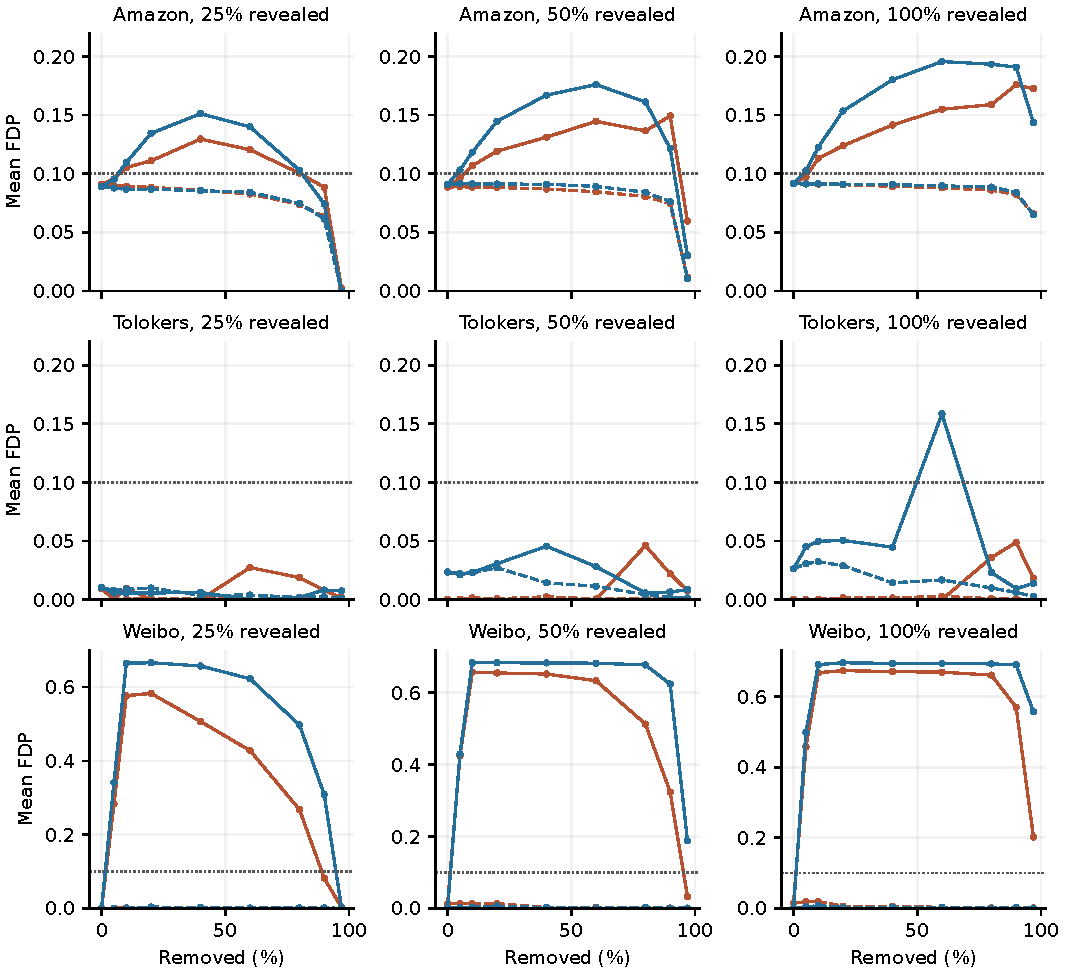
\includegraphics[width=.96\textwidth]{selection_dose_all_fdp.pdf}
\caption{Complete removal grid: mean FDP over training-seed averages, including abstention. Orange is attributes; blue adds graph features. Solid lines remove by observed exposure; dashed lines remove uniformly. Every cell uses ten training seeds, five splits, and 50 paired repetitions. Different graphs may have different vertical scales.}
\label{fig:doseallfdp}\end{figure}
\clearpage\begin{figure}[p]\centering
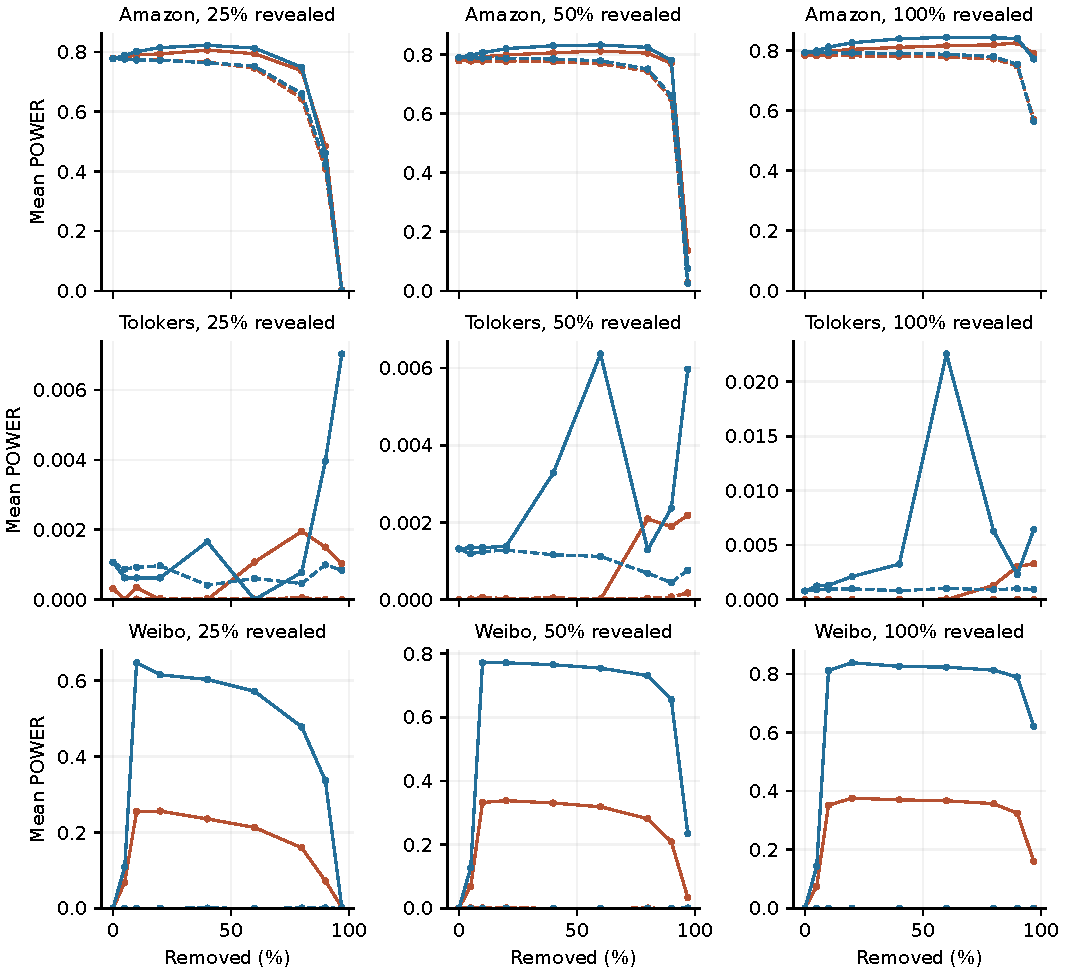
\includegraphics[width=.96\textwidth]{selection_dose_all_power.pdf}
\caption{Complete removal grid: mean POWER over training-seed averages, including abstention. Orange is attributes; blue adds graph features. Solid lines remove by observed exposure; dashed lines remove uniformly. Every cell uses ten training seeds, five splits, and 50 paired repetitions. Different graphs may have different vertical scales.}
\label{fig:doseallpower}\end{figure}

\clearpage\section{T-FINANCE AND WEIBO SOURCE SENSITIVITY}
\label{app:extensions}
\paragraph{Protocol and acquisition.}
The T-Finance protocol was saved before loading model outcomes. We downloaded the T-Finance and Weibo members of the official GADBench archive~\citep{tang2023gadbench}, verified ZIP CRC and SHA-256, and retained their distributed binary labels and numerical features without relabeling. Raw adjacency is symmetrized, binarized, and stripped of self loops. T-Finance has 39,357 nodes, 10 features, 1,803 anomalous labels and 21,222,543 undirected edges. GADBench Weibo has 8,405 nodes, 400 features, 868 anomalous labels and 377,271 undirected edges. Original GADBench train/validation/test masks are not used; we apply the same uniform 10\% training-panel design as the other controls.

\paragraph{Weibo provenance.}
The actual official PyGOD file has 347 anomalous labels despite its README's stated 868. A fresh download is byte-identical to our raw input, and the cached labels equal those distributed labels. The separately distributed GADBench file has 868 anomalous labels. The two raw feature matrices agree entrywise and their symmetrized, loop-free adjacency matrices agree. Two nodes share identical features and symmetric neighborhoods, so external node identities are not established uniquely from those arrays alone. The existing PyGOD processed cache standardizes features; this source extension preserves GADBench's raw distributed features. We therefore report a source sensitivity, not a claim that every numerical difference isolates label changes alone. PyGOD and GADBench outcomes are never pooled.

The raw GADBench Weibo SHA-256 is
\texttt{111402a2cb3b6a10\allowbreak ec586e96122da809\allowbreak d62bfe3617add07cb\allowbreak 006de53fc109f05};
T-Finance is
\texttt{8f3b05272703220b\allowbreak b3248b0caac92e91\allowbreak 7c7524704094c02f\allowbreak 802b400026ed1d38}.
The machine-readable provenance includes full hashes, upstream commit, download ranges, actual field shapes and processed-graph hashes.

\paragraph{Training and evaluation.}
For each graph, fit ten attribute-only and ten graph-feature histogram-gradient-boosting scorers with the fixed settings in Appendix~\ref{app:supervised}. T-Finance has 3,936 training labels and GADBench Weibo has 840. Training labels never re-enter calibration or testing. All calculations use sparse adjacency and CPU training. Each extension retains five test splits, three label-revelation fractions, nine removal fractions, two matched rules and fifty calibration repetitions: 270,000 evaluations per source. The Weibo sensitivity uses the earlier Weibo RNG namespace, while T-Finance uses a new dataset index; class-stratified test identities can change when source labels differ. All results, including abstentions and unsuccessful contrasts, are retained. Neither score direction nor hyperparameters are selected using these outcomes.

\begin{table*}[t]\centering\small
\caption{Prespecified 20\%-removal comparison with half of non-test labels revealed. FDP/power pairs average all outcomes; ranking metrics average ten training seeds. Full curves follow.}
\begin{tabular}{llrrrr}\toprule Graph & Score & AUROC & AP & Exposure FDP/power & Random FDP/power\\\midrule
T-Finance & Attributes & $0.940$ & $0.794$ & $0.127/0.668$ & $0.093/0.650$ \\
T-Finance & Graph features & $0.962$ & $0.880$ & $0.191/0.830$ & $0.095/0.789$ \\
Weibo (GADBench) & Attributes & $0.982$ & $0.899$ & $0.184/0.783$ & $0.094/0.663$ \\
Weibo (GADBench) & Graph features & $0.993$ & $0.954$ & $0.286/0.973$ & $0.091/0.844$ \\
\bottomrule\end{tabular}\end{table*}

\begin{figure*}[t]\centering
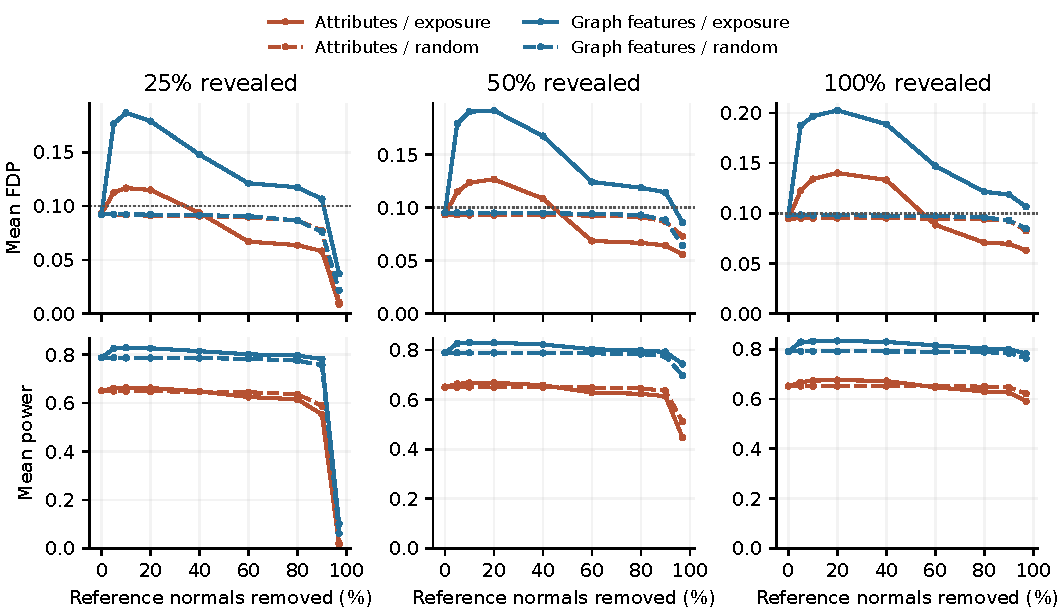
\includegraphics[width=\textwidth]{extension_dose_tfinance.pdf}
\caption{T-Finance: complete prespecified removal sweep. Both scorers, all nine removal fractions and all three revelation fractions are shown. Solid lines use exposure removal; dashed lines use equally sized random references. Means retain every abstention and average ten training-seed means.}
\end{figure*}

\begin{figure*}[t]\centering
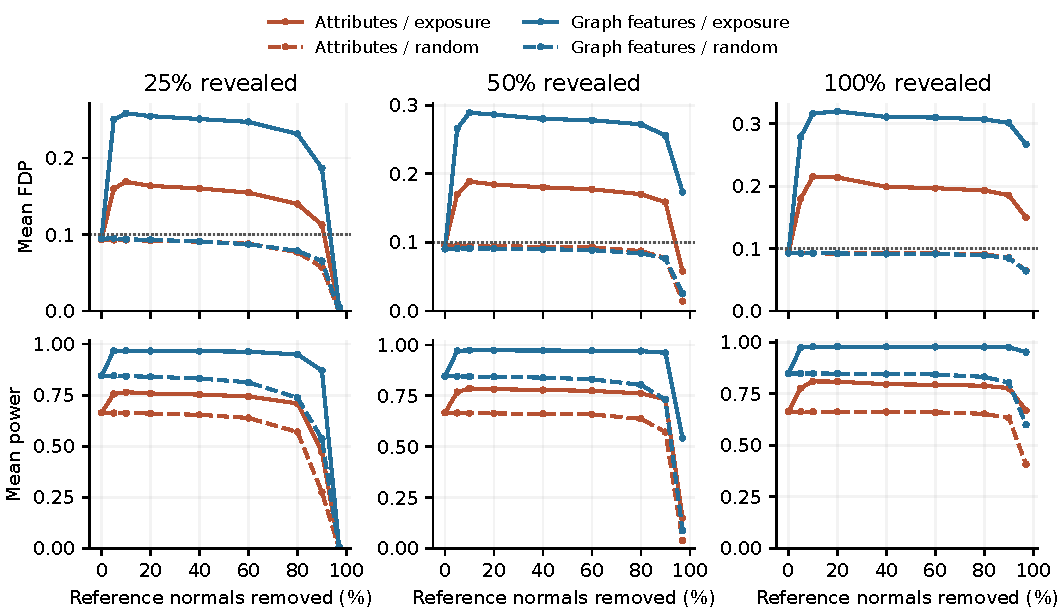
\includegraphics[width=\textwidth]{extension_dose_weibo_gadbench.pdf}
\caption{Weibo (GADBench): complete prespecified removal sweep. Both scorers, all nine removal fractions and all three revelation fractions are shown. Solid lines use exposure removal; dashed lines use equally sized random references. Means retain every abstention and average ten training-seed means.}
\end{figure*}
\clearpage\section{STRATIFIED RANDOM-ROLE CALIBRATION}
\label{app:stratified}
\paragraph{A remedy based on randomized roles.}
Rather than use a low-exposure reference for every test node, retain both exposure strata and calibrate each against its own randomly acquired normals. Fix the strata using the graph, a separate training panel, and observed anomalous neighbors. Their construction must be invariant to which remaining normal nodes become calibration or test nodes. A threshold estimated only from the realized calibration pool generally does not meet this requirement.

\begin{lemma}[Stratified random-role calibration]
\label{lem:stratified}
Condition on the graph, labels, deployment universe, training panel, role-invariant fitted scores, and all anomaly-side test and revelation assignments. Let $D_1,\ldots,D_H$ be strata fixed by this information. Resolve all score ties lexicographically with independent continuous marks drawn before normal-role assignment. Uniformly choose a prescribed number of deployment normals for testing, and independently reveal each remaining normal with probability $\rho$. In stratum $h$, let $n_h$ be the revealed-normal reference size, $m_{0h}$ the normal-test count, and $m_h$ the total test count. Apply conformal BH separately at fixed levels $\alpha_h$ with $\sum_h\alpha_h\le\alpha$, abstaining if the reference or test stratum is empty. Conditional also on all stratum role counts,
\begin{equation}
\E[\FDP_{\rm union}]
\le\sum_{h:m_h>0}\alpha_h\frac{m_{0h}}{m_h}\le\alpha.
\label{eq:stratified}
\end{equation}
\end{lemma}
The conditional expectation in Equation~\eqref{eq:stratified} averages over normal identities assigned to roles; it does not fix the realized normal test set. Uniform role assignment supplies the exchangeability needed within each stratum~\citep{marandon2024adaptive}. Splitting $\alpha$ avoids a cross-stratum dependence assumption because $\FDP_{\rm union}\le\sum_h\FDP_h$ pointwise. Small strata reduce rank resolution and power, while empty references safely abstain. The proof and the comparisons with pooled full-reference calibration follow.

\paragraph{Conditioning and construction.}
Let $\mathcal F$ include the finite graph, its entire fixed label vector, the training panel, the deployment universe, fitted scores unchanged by normal-role reassignment, and every anomalous node's test/revelation assignment. It also includes independent continuous score tie marks and any auxiliary marks used to break exposure ties, drawn before normal-role assignment. The partition $D_1,\ldots,D_H$ is $\mathcal F$-measurable. This conditioning is a design-based analysis; the procedure does not observe hidden test labels.

For example, the numerator of observed exposure counts anomalous neighbors known from the training and revealed non-test panels. Conditional on their assignments it is fixed; division by the graph's fixed degree preserves this property. Changing which normal neighbors are revealed contributes zero to the numerator. By contrast, dividing by the number of revealed neighbors, or choosing a threshold from just the realized normal reference, can make the partition depend on normal roles and requires another argument.

\paragraph{Proof of Lemma~\ref{lem:stratified}.}
Write $N$ for the number of deployment normals and $t$ for the prescribed normal-test count. For $0<\rho<1$, a particular normal-role partition into test nodes $T_0$, revealed reference nodes $C$, and unused nodes $U$ has probability
\[
\binom Nt^{-1}\rho^{|C|}(1-\rho)^{|U|}.
\]
This probability is constant over assignments having the same role counts in each fixed stratum. Thus, conditional on $\mathcal F$ and those counts, normal identities are exchangeable among the roles within each stratum. At $\rho=0$ or $1$, the same statement holds on the feasible assignments directly. Anomaly-side and normal-side sampling must have this conditional law; conditioning on an arbitrary coupled allocation would not establish it.

Fix a stratum and additionally condition on the unordered set of normals occupying calibration and null-test roles. Assign them to calibration and null-test positions, introducing independent random orderings within each group. Every permutation into those positions is equally likely. Hence their score vector is jointly exchangeable conditional on the anomalous test scores. Auxiliary ordering does not alter any p-value attached to a node or the FDP. Lexicographic tie marks make every calibration and test score distinct; equivalently use ranks in this fixed total ordering. The score-level exchangeability result of \citet[Theorem 3.3]{marandon2024adaptive} supplies null super-uniformity and PRDS within this stratum. BH therefore gives
\[
\E[\FDP_h\mid\mathcal F,\mathcal K]
\le\alpha_h m_{0h}/m_h,
\]
after averaging over the additional unordered-set conditioning, where $\mathcal K$ denotes all stratum role counts. Empty references abstain, and empty test strata have FDP zero.

Let $R_h$ and $V_h$ be the discovery and false-discovery counts. For every realization,
\[
\frac{\sum_h V_h}{(\sum_h R_h)\vee1}
\le\sum_h\frac{V_h}{R_h\vee1}.
\]
Taking conditional expectations proves Equation~\eqref{eq:stratified}. No independence or PRDS condition across strata is invoked. The strata and level allocation must be fixed under the stated conditioning; selecting them after inspecting FDP is not covered.

\paragraph{Prespecified empirical comparison.}
We use two separate binary partitions: zero versus positive observed exposure, and the lower 80\% versus upper 20\% of exposure ranks over the entire deployment universe. Independent continuous marks break exposure ties in the latter. Its cutoff is fixed under normal-role permutations, unlike a cutoff computed from only calibration normals. Neither partition is selected based on its results. Each stratum receives level $0.05$, including when another stratum is empty.

For each graph, both frozen supervised scorers, all ten training seeds, five test splits, and revealed fractions $0.25,0.50,1$, we compare pooled full-reference BH at $0.10$, low-stratum calibration applied to the entire test set at $0.10$, and separate-stratum BH. Full-reference and stratified calibration use the same total acquired labels and reference nodes. The low-stratum diagnostic uses fewer references; the separate dose experiment supplies size-matched composition comparisons. We retain every result, including power losses and abstentions.

\paragraph{Implementation checks.}
Enumeration over 44,256 joint role assignments checks both the stratum-level BH bound and the union bound; 16,110 assignments have nonempty discoveries. Two hundred tied-score examples compare rank-based BH with a direct reference implementation. Empty references abstain. For each evaluated split and revelation fraction, altering unknown labels or normal revelation roles leaves exposure unchanged; both partition constructions are checked for the same invariance. The protocol, per-split outcomes, seed summaries and input hashes are included in the supplement.

\begin{table*}[t]\centering\small
\caption{Amazon: complete stratified comparison, mean FDP / power over ten training-seed averages. Both partitions and all revelation fractions are shown; no partition is selected using these outcomes.}
\begin{tabular}{lllrrr}\toprule Score & $\rho$ & Partition & Low reference & Full random & Stratified\\\midrule
Attributes & 0.25 & Zero/positive & $0.093/0.679$ & $0.091/0.779$ & $0.039/0.567$ \\
Attributes & 0.25 & 80/20 ranks & $0.110/0.793$ & $0.091/0.779$ & $0.036/0.530$ \\
Attributes & 0.50 & Zero/positive & $0.140/0.770$ & $0.089/0.779$ & $0.042/0.651$ \\
Attributes & 0.50 & 80/20 ranks & $0.114/0.797$ & $0.089/0.779$ & $0.039/0.581$ \\
Attributes & 1.00 & Zero/positive & $0.198/0.807$ & $0.092/0.783$ & $0.044/0.694$ \\
Attributes & 1.00 & 80/20 ranks & $0.118/0.800$ & $0.092/0.783$ & $0.038/0.637$ \\
Graph & 0.25 & Zero/positive & $0.085/0.675$ & $0.089/0.778$ & $0.047/0.572$ \\
Graph & 0.25 & 80/20 ranks & $0.127/0.813$ & $0.089/0.778$ & $0.038/0.509$ \\
Graph & 0.50 & Zero/positive & $0.118/0.756$ & $0.091/0.791$ & $0.045/0.665$ \\
Graph & 0.50 & 80/20 ranks & $0.132/0.814$ & $0.091/0.791$ & $0.040/0.579$ \\
Graph & 1.00 & Zero/positive & $0.155/0.791$ & $0.091/0.793$ & $0.046/0.697$ \\
Graph & 1.00 & 80/20 ranks & $0.139/0.818$ & $0.091/0.793$ & $0.034/0.639$ \\
\bottomrule\end{tabular}\end{table*}

\begin{table*}[t]\centering\small
\caption{Tolokers: complete stratified comparison, mean FDP / power over ten training-seed averages. Both partitions and all revelation fractions are shown; no partition is selected using these outcomes.}
\begin{tabular}{lllrrr}\toprule Score & $\rho$ & Partition & Low reference & Full random & Stratified\\\midrule
Attributes & 0.25 & Zero/positive & $0.028/0.002$ & $0.009/0.000$ & $0.000/0.000$ \\
Attributes & 0.25 & 80/20 ranks & $0.000/0.000$ & $0.009/0.000$ & $0.000/0.000$ \\
Attributes & 0.50 & Zero/positive & $0.057/0.003$ & $0.000/0.000$ & $0.000/0.000$ \\
Attributes & 0.50 & 80/20 ranks & $0.000/0.000$ & $0.000/0.000$ & $0.000/0.000$ \\
Attributes & 1.00 & Zero/positive & $0.065/0.003$ & $0.000/0.000$ & $0.000/0.000$ \\
Attributes & 1.00 & 80/20 ranks & $0.000/0.000$ & $0.000/0.000$ & $0.000/0.000$ \\
Graph & 0.25 & Zero/positive & $0.000/0.000$ & $0.010/0.001$ & $0.000/0.000$ \\
Graph & 0.25 & 80/20 ranks & $0.006/0.001$ & $0.010/0.001$ & $0.000/0.000$ \\
Graph & 0.50 & Zero/positive & $0.005/0.001$ & $0.023/0.001$ & $0.000/0.000$ \\
Graph & 0.50 & 80/20 ranks & $0.040/0.002$ & $0.023/0.001$ & $0.000/0.000$ \\
Graph & 1.00 & Zero/positive & $0.005/0.001$ & $0.026/0.001$ & $0.004/0.000$ \\
Graph & 1.00 & 80/20 ranks & $0.044/0.002$ & $0.026/0.001$ & $0.000/0.000$ \\
\bottomrule\end{tabular}\end{table*}

\begin{table*}[t]\centering\small
\caption{Weibo (PyGOD): complete stratified comparison, mean FDP / power over ten training-seed averages. Both partitions and all revelation fractions are shown; no partition is selected using these outcomes.}
\begin{tabular}{lllrrr}\toprule Score & $\rho$ & Partition & Low reference & Full random & Stratified\\\midrule
Attributes & 0.25 & Zero/positive & $0.590/0.260$ & $0.000/0.000$ & $0.000/0.000$ \\
Attributes & 0.25 & 80/20 ranks & $0.592/0.262$ & $0.000/0.000$ & $0.000/0.000$ \\
Attributes & 0.50 & Zero/positive & $0.656/0.343$ & $0.013/0.001$ & $0.000/0.000$ \\
Attributes & 0.50 & 80/20 ranks & $0.656/0.342$ & $0.013/0.001$ & $0.000/0.000$ \\
Attributes & 1.00 & Zero/positive & $0.675/0.371$ & $0.015/0.000$ & $0.000/0.000$ \\
Attributes & 1.00 & 80/20 ranks & $0.676/0.373$ & $0.015/0.000$ & $0.000/0.000$ \\
Graph & 0.25 & Zero/positive & $0.666/0.629$ & $0.000/0.000$ & $0.000/0.000$ \\
Graph & 0.25 & 80/20 ranks & $0.666/0.630$ & $0.000/0.000$ & $0.000/0.000$ \\
Graph & 0.50 & Zero/positive & $0.683/0.768$ & $0.000/0.000$ & $0.000/0.000$ \\
Graph & 0.50 & 80/20 ranks & $0.684/0.774$ & $0.000/0.000$ & $0.000/0.000$ \\
Graph & 1.00 & Zero/positive & $0.695/0.826$ & $0.000/0.000$ & $0.000/0.000$ \\
Graph & 1.00 & 80/20 ranks & $0.697/0.843$ & $0.000/0.000$ & $0.000/0.000$ \\
\bottomrule\end{tabular}\end{table*}

\begin{table*}[t]\centering\small
\caption{T-Finance: complete stratified comparison, mean FDP / power over ten training-seed averages. Both partitions and all revelation fractions are shown; no partition is selected using these outcomes.}
\begin{tabular}{lllrrr}\toprule Score & $\rho$ & Partition & Low reference & Full random & Stratified\\\midrule
Attributes & 0.25 & Zero/positive & $0.067/0.627$ & $0.093/0.650$ & $0.046/0.633$ \\
Attributes & 0.25 & 80/20 ranks & $0.119/0.665$ & $0.093/0.650$ & $0.037/0.623$ \\
Attributes & 0.50 & Zero/positive & $0.067/0.626$ & $0.093/0.651$ & $0.045/0.633$ \\
Attributes & 0.50 & 80/20 ranks & $0.127/0.669$ & $0.093/0.651$ & $0.037/0.628$ \\
Attributes & 1.00 & Zero/positive & $0.071/0.633$ & $0.095/0.652$ & $0.045/0.629$ \\
Attributes & 1.00 & 80/20 ranks & $0.138/0.675$ & $0.095/0.652$ & $0.037/0.629$ \\
Graph & 0.25 & Zero/positive & $0.123/0.803$ & $0.092/0.787$ & $0.043/0.744$ \\
Graph & 0.25 & 80/20 ranks & $0.182/0.827$ & $0.092/0.787$ & $0.038/0.731$ \\
Graph & 0.50 & Zero/positive & $0.122/0.803$ & $0.095/0.789$ & $0.044/0.751$ \\
Graph & 0.50 & 80/20 ranks & $0.192/0.830$ & $0.095/0.789$ & $0.038/0.737$ \\
Graph & 1.00 & Zero/positive & $0.121/0.804$ & $0.099/0.792$ & $0.046/0.753$ \\
Graph & 1.00 & 80/20 ranks & $0.202/0.834$ & $0.099/0.792$ & $0.038/0.738$ \\
\bottomrule\end{tabular}\end{table*}

\begin{table*}[t]\centering\small
\caption{Weibo (GADBench): complete stratified comparison, mean FDP / power over ten training-seed averages. Both partitions and all revelation fractions are shown; no partition is selected using these outcomes.}
\begin{tabular}{lllrrr}\toprule Score & $\rho$ & Partition & Low reference & Full random & Stratified\\\midrule
Attributes & 0.25 & Zero/positive & $0.164/0.758$ & $0.093/0.664$ & $0.025/0.478$ \\
Attributes & 0.25 & 80/20 ranks & $0.168/0.764$ & $0.093/0.664$ & $0.017/0.401$ \\
Attributes & 0.50 & Zero/positive & $0.181/0.779$ & $0.096/0.666$ & $0.036/0.537$ \\
Attributes & 0.50 & 80/20 ranks & $0.189/0.787$ & $0.096/0.666$ & $0.025/0.489$ \\
Attributes & 1.00 & Zero/positive & $0.198/0.795$ & $0.093/0.664$ & $0.042/0.559$ \\
Attributes & 1.00 & 80/20 ranks & $0.216/0.811$ & $0.093/0.664$ & $0.026/0.495$ \\
Graph & 0.25 & Zero/positive & $0.253/0.966$ & $0.094/0.845$ & $0.030/0.571$ \\
Graph & 0.25 & 80/20 ranks & $0.258/0.969$ & $0.094/0.845$ & $0.023/0.474$ \\
Graph & 0.50 & Zero/positive & $0.280/0.972$ & $0.090/0.846$ & $0.029/0.630$ \\
Graph & 0.50 & 80/20 ranks & $0.290/0.974$ & $0.090/0.846$ & $0.020/0.523$ \\
Graph & 1.00 & Zero/positive & $0.311/0.978$ & $0.093/0.848$ & $0.035/0.673$ \\
Graph & 1.00 & 80/20 ranks & $0.317/0.978$ & $0.093/0.848$ & $0.023/0.567$ \\
\bottomrule\end{tabular}\end{table*}

\paragraph{Stratification restores a guarantee, with a power cost.}
The random-role remedy uses both exposure strata and divides $\alpha$ equally between them. With half of non-test labels revealed, the Amazon attribute scorer gives mean FDP $0.042$ and power $0.651$ for zero/positive-exposure strata, versus $0.089$ and $0.779$ for the pooled full random reference. The graph-feature scorer gives $0.045/0.665$ versus $0.091/0.791$. Thus the remedy supplies a design-based guarantee but does not outperform representative pooled calibration here. The 80/20 exposure partition and all other conditions are retained in Appendix~\ref{app:stratified}. These cutoffs are fixed under normal-role changes, so their filtered comparisons differ from the reference-quantile dose intervention.

\clearpage\section{ERROR ALLOCATION AND SELECTED LABEL ACQUISITION}
\label{app:allocation}
\paragraph{Stratum-size allocation.}
In Lemma~\ref{lem:stratified}, the realized $m_h$ need not be fixed before normal roles are drawn. They are fixed after conditioning on the stratum role counts $\mathcal K$. Setting $\alpha_h=\alpha m_h/m$ therefore gives
\[
\E[\FDP_{\rm union}\mid\mathcal F,\mathcal K]
\le \sum_{h:m_h>0}\frac{\alpha m_h}{m}\frac{m_{0h}}{m_h}
=\alpha\frac{m_0}{m}.
\]
This is an allocation rule, not a power ordering relative to equal allocation.

\paragraph{One BH across stratified ranks.}
Suppose normal reference revelation has a fixed probability $\rho_h$ within each fixed stratum, independently across nodes. For a feasible assignment of normal identities to test, reference and unused roles, its probability conditional on $\mathcal F$ is
\[
\binom Nt^{-1}\prod_h\rho_h^{n_h}(1-\rho_h)^{u_h}.
\]
Given $\mathcal K$, this is constant over a Cartesian product of the feasible within-stratum assignments. Its normalizing constant factors over that product. Consequently the within-stratum role assignments are independent under this conditioning. This independence follows from randomized roles on the fixed graph, not from independence of graph observations. It would not hold automatically for an arbitrary adaptive acquisition policy.

In each stratum, introduce independent random orderings of calibration and null-test positions as in the proof of Lemma~\ref{lem:stratified}. The conditional exchangeability theorem supplies super-uniform null ranks and PRDS within each block~\citep[Theorem 3.3]{marandon2024adaptive}. An empty-reference block has constant p-values equal to one. Independent PRDS blocks are jointly PRDS: for a null coordinate in block $h$ and any coordinatewise increasing set $A$, fix the other blocks. Its section in block $h$ is increasing, so its conditional probability is nondecreasing in that null p-value. Average over the independent other blocks; their law does not change with the conditioned coordinate. This preserves the monotonicity. Thus one BH at $\alpha$ on all stratum-wise p-values satisfies
\[
\E[\FDP_{\rm pooled\ strata}\mid\mathcal F,\mathcal K]
\le\alpha m_0/m.
\]
The artificial ordering of positions changes neither the rejection set nor FDP. Averaging over counts preserves the bound. This result strengthens the allocation argument only for the specified product sampling design; the earlier sum-FDP argument remains applicable without cross-stratum independence.

\paragraph{Known-propensity weighting.}
For the biased-acquisition experiment, strata and probabilities are fixed using only training labels and graph features. Assign a prescribed total number of normal test positions uniformly, then acquire each remaining normal with probability $\rho(v)=\rho_{h(v)}>0$. Consider one designated null test position. Condition on all other null test identities, the unordered union $S$ of its node and calibration nodes, and the unused nodes; do not additionally fix this designated position's stratum. For a possible target $j\in S$, assignment probability is proportional to
\[
\prod_{i\in S\setminus\{j\}}\rho(i)
=\frac{\prod_{i\in S}\rho(i)}{\rho(j)}.
\]
Uniform test-position assignment and the probabilities of unused nodes contribute common factors. Conditional target mass is therefore proportional to $w(j)=1/\rho(j)$. Summing this mass over nodes with score at least the target score yields
\[
p_w(v)=\frac{w(v)+\sum_{u\in C}w(u)\ind\{s(u)\ge s(v)\}}
{w(v)+\sum_{u\in C}w(u)}.
\]
The cumulative-mass argument gives marginal null super-uniformity; an empty reference returns one. This is the weighted-exchangeability principle~\citep{tibshirani2019conformal} applied to the acquisition design. BY at $\alpha/\sum_{j=1}^m1/j$ consequently controls FDR under arbitrary p-value dependence~\citep{benjamini2001control}. Weighted BH is retained as a descriptive comparator: the marginal argument does not establish its joint PRDS condition. These probabilities are known by design, not estimated propensities for an arbitrary analyst policy.

\begin{figure*}[t]
\centering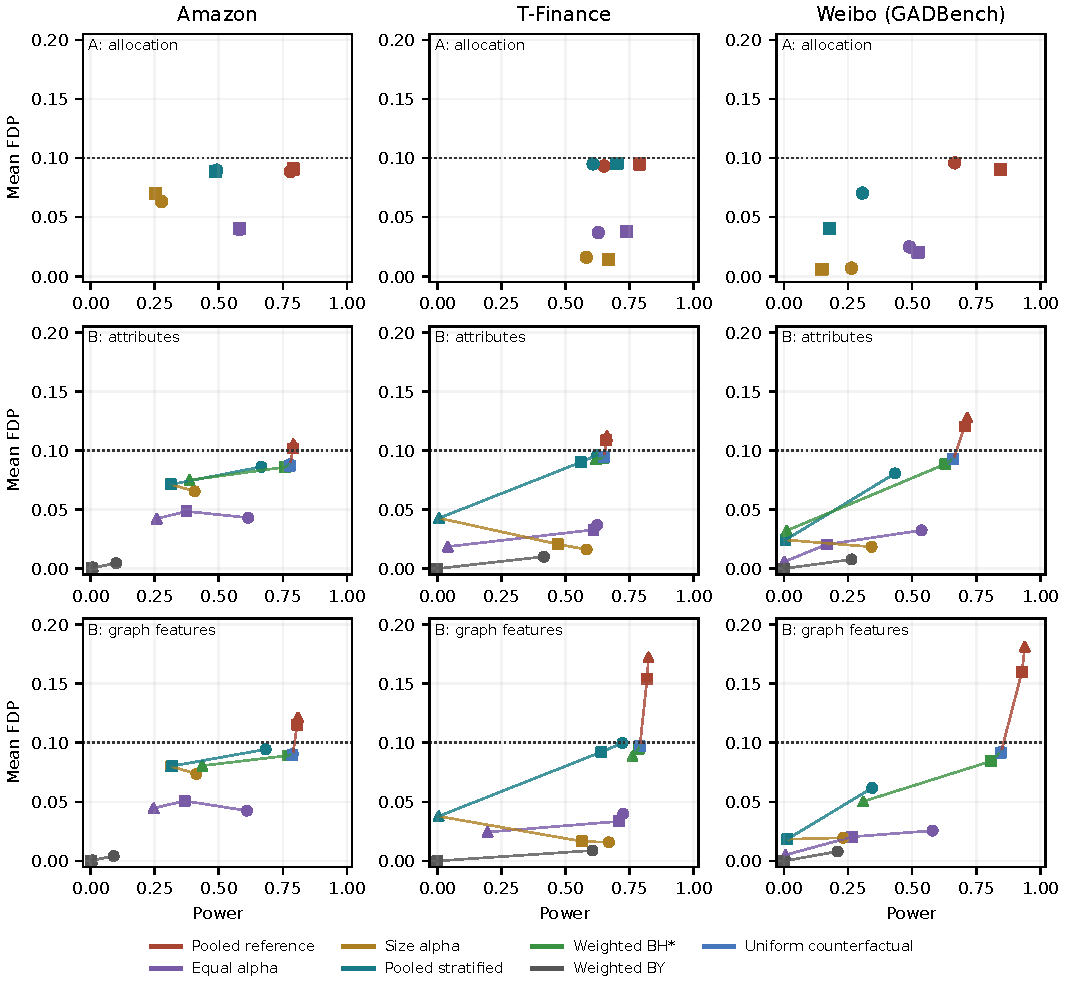
\includegraphics[width=\textwidth]{allocation_acquisition.pdf}
\caption{FDP versus power for the prespecified 80/20 partition. Top: uniform acquisition at half revelation, comparing allocation rules; circles/squares denote attribute/graph scorers. Middle and bottom: biased acquisition with attribute and graph scorers. Circles, squares and triangles follow neutral, moderate and severe acquisition bias; lines connect those settings, not a tuned frontier. Dotted lines mark nominal $0.10$. Weighted BH* has no joint guarantee established here. Uniform acquisition is a counterfactual, not an available reference within the biased-design scenario. All methods share scores and test identities; means include abstentions.}
\label{fig:allocationfull}
\end{figure*}

The follow-up protocol was frozen after the equal-alpha results, before these variants were evaluated. It is an exploratory follow-up. Phase A reproduces 5,400 previously stored outcomes before comparing allocations. Phase B fixes exposure using only training labels and graph degree, then independently acquires each non-test node's label with the stated stratum probability. Acquired anomalies count toward label cost but are not normal references. Strata are never updated with newly acquired labels. The uniform counterfactual uses the deployment-universe mean acquisition probability, fixed before normal-role assignment; costs are close in expectation, not matched exactly per realization. Each phase retains all ten training seeds and five splits; phase B adds ten acquisition repetitions. The full ledger has 135,000 procedure evaluations.

All means include abstentions. Pointwise paired intervals over ten seed averages are supplied in the result CSVs; they do not quantify cross-graph uncertainty. Exact small-design checks include 6,246 conditional block assignments with nonzero false-discovery events, and 11,264 unequal-propensity assignments for marginal weighted ranks. These checks support implementation verification and do not replace the argument above.

\begin{table*}[t]\centering\scriptsize\setlength{\tabcolsep}{3pt}
\caption{Amazon, allocation: mean FDP / power. Every declared partition and setting is shown. For acquisition, neu/mod/sev denote $(\rho_L,\rho_H)=(.5,.5),(.5,.1),(.5,.025)$. W-BH* is descriptive; its marginal-rank argument is not a BH guarantee. Uniform is a counterfactual acquisition design.}
\begin{tabular}{lllrrrrr}\toprule Score & Strata & Setting & Pooled & Equal & Size & Joint & Low only\\\midrule
Attr. & Zero & 0.25 & $0.091/0.779$ & $0.039/0.567$ & $0.072/0.655$ & $0.081/0.755$ & $0.093/0.679$ \\
Attr. & Zero & 0.50 & $0.089/0.779$ & $0.042/0.651$ & $0.078/0.714$ & $0.088/0.774$ & $0.140/0.770$ \\
Attr. & Zero & 1.00 & $0.092/0.783$ & $0.044/0.694$ & $0.088/0.758$ & $0.092/0.781$ & $0.198/0.807$ \\
Attr. & 80/20 & 0.25 & $0.091/0.779$ & $0.036/0.530$ & $0.055/0.182$ & $0.070/0.404$ & $0.110/0.793$ \\
Attr. & 80/20 & 0.50 & $0.089/0.779$ & $0.039/0.581$ & $0.063/0.277$ & $0.090/0.492$ & $0.114/0.797$ \\
Attr. & 80/20 & 1.00 & $0.092/0.783$ & $0.038/0.637$ & $0.054/0.287$ & $0.094/0.551$ & $0.118/0.800$ \\
Graph & Zero & 0.25 & $0.089/0.778$ & $0.047/0.572$ & $0.073/0.645$ & $0.081/0.751$ & $0.085/0.675$ \\
Graph & Zero & 0.50 & $0.091/0.791$ & $0.045/0.665$ & $0.080/0.716$ & $0.089/0.781$ & $0.118/0.756$ \\
Graph & Zero & 1.00 & $0.091/0.793$ & $0.046/0.697$ & $0.088/0.764$ & $0.089/0.789$ & $0.155/0.791$ \\
Graph & 80/20 & 0.25 & $0.089/0.778$ & $0.038/0.509$ & $0.065/0.212$ & $0.082/0.457$ & $0.127/0.813$ \\
Graph & 80/20 & 0.50 & $0.091/0.791$ & $0.040/0.579$ & $0.070/0.252$ & $0.089/0.487$ & $0.132/0.814$ \\
Graph & 80/20 & 1.00 & $0.091/0.793$ & $0.034/0.639$ & $0.073/0.258$ & $0.096/0.516$ & $0.139/0.818$ \\
\bottomrule\end{tabular}\end{table*}

\begin{table*}[t]\centering\scriptsize\setlength{\tabcolsep}{3pt}
\caption{T-Finance, allocation: mean FDP / power. Every declared partition and setting is shown. For acquisition, neu/mod/sev denote $(\rho_L,\rho_H)=(.5,.5),(.5,.1),(.5,.025)$. W-BH* is descriptive; its marginal-rank argument is not a BH guarantee. Uniform is a counterfactual acquisition design.}
\begin{tabular}{lllrrrrr}\toprule Score & Strata & Setting & Pooled & Equal & Size & Joint & Low only\\\midrule
Attr. & Zero & 0.25 & $0.093/0.650$ & $0.046/0.633$ & $0.051/0.638$ & $0.090/0.658$ & $0.067/0.627$ \\
Attr. & Zero & 0.50 & $0.093/0.651$ & $0.045/0.633$ & $0.056/0.646$ & $0.092/0.660$ & $0.067/0.626$ \\
Attr. & Zero & 1.00 & $0.095/0.652$ & $0.045/0.629$ & $0.063/0.647$ & $0.093/0.658$ & $0.071/0.633$ \\
Attr. & 80/20 & 0.25 & $0.093/0.650$ & $0.037/0.623$ & $0.014/0.567$ & $0.093/0.607$ & $0.119/0.665$ \\
Attr. & 80/20 & 0.50 & $0.093/0.651$ & $0.037/0.628$ & $0.016/0.581$ & $0.095/0.608$ & $0.127/0.669$ \\
Attr. & 80/20 & 1.00 & $0.095/0.652$ & $0.037/0.629$ & $0.015/0.577$ & $0.100/0.603$ & $0.138/0.675$ \\
Graph & Zero & 0.25 & $0.092/0.787$ & $0.043/0.744$ & $0.048/0.752$ & $0.092/0.775$ & $0.123/0.803$ \\
Graph & Zero & 0.50 & $0.095/0.789$ & $0.044/0.751$ & $0.056/0.766$ & $0.095/0.784$ & $0.122/0.803$ \\
Graph & Zero & 1.00 & $0.099/0.792$ & $0.046/0.753$ & $0.065/0.776$ & $0.098/0.789$ & $0.121/0.804$ \\
Graph & 80/20 & 0.25 & $0.092/0.787$ & $0.038/0.731$ & $0.012/0.648$ & $0.090/0.690$ & $0.182/0.827$ \\
Graph & 80/20 & 0.50 & $0.095/0.789$ & $0.038/0.737$ & $0.014/0.668$ & $0.095/0.701$ & $0.192/0.830$ \\
Graph & 80/20 & 1.00 & $0.099/0.792$ & $0.038/0.738$ & $0.013/0.676$ & $0.101/0.708$ & $0.202/0.834$ \\
\bottomrule\end{tabular}\end{table*}

\begin{table*}[t]\centering\scriptsize\setlength{\tabcolsep}{3pt}
\caption{Weibo (GADBench), allocation: mean FDP / power. Every declared partition and setting is shown. For acquisition, neu/mod/sev denote $(\rho_L,\rho_H)=(.5,.5),(.5,.1),(.5,.025)$. W-BH* is descriptive; its marginal-rank argument is not a BH guarantee. Uniform is a counterfactual acquisition design.}
\begin{tabular}{lllrrrrr}\toprule Score & Strata & Setting & Pooled & Equal & Size & Joint & Low only\\\midrule
Attr. & Zero & 0.25 & $0.093/0.664$ & $0.025/0.478$ & $0.011/0.260$ & $0.048/0.284$ & $0.164/0.758$ \\
Attr. & Zero & 0.50 & $0.096/0.666$ & $0.036/0.537$ & $0.020/0.443$ & $0.086/0.466$ & $0.181/0.779$ \\
Attr. & Zero & 1.00 & $0.093/0.664$ & $0.042/0.559$ & $0.032/0.519$ & $0.096/0.536$ & $0.198/0.795$ \\
Attr. & 80/20 & 0.25 & $0.093/0.664$ & $0.017/0.401$ & $0.001/0.013$ & $0.010/0.049$ & $0.168/0.764$ \\
Attr. & 80/20 & 0.50 & $0.096/0.666$ & $0.025/0.489$ & $0.007/0.263$ & $0.070/0.306$ & $0.189/0.787$ \\
Attr. & 80/20 & 1.00 & $0.093/0.664$ & $0.026/0.495$ & $0.009/0.377$ & $0.089/0.384$ & $0.216/0.811$ \\
Graph & Zero & 0.25 & $0.094/0.845$ & $0.030/0.571$ & $0.012/0.286$ & $0.056/0.322$ & $0.253/0.966$ \\
Graph & Zero & 0.50 & $0.090/0.846$ & $0.029/0.630$ & $0.016/0.457$ & $0.072/0.474$ & $0.280/0.972$ \\
Graph & Zero & 1.00 & $0.093/0.848$ & $0.035/0.673$ & $0.029/0.622$ & $0.090/0.637$ & $0.311/0.978$ \\
Graph & 80/20 & 0.25 & $0.094/0.845$ & $0.023/0.474$ & $0.005/0.066$ & $0.019/0.093$ & $0.258/0.969$ \\
Graph & 80/20 & 0.50 & $0.090/0.846$ & $0.020/0.523$ & $0.006/0.148$ & $0.041/0.178$ & $0.290/0.974$ \\
Graph & 80/20 & 1.00 & $0.093/0.848$ & $0.023/0.567$ & $0.007/0.204$ & $0.061/0.249$ & $0.317/0.978$ \\
\bottomrule\end{tabular}\end{table*}

\begin{table*}[t]\centering\scriptsize\setlength{\tabcolsep}{3pt}
\caption{Amazon, acquisition: mean FDP / power. Every declared partition and setting is shown. For acquisition, neu/mod/sev denote $(\rho_L,\rho_H)=(.5,.5),(.5,.1),(.5,.025)$. W-BH* is descriptive; its marginal-rank argument is not a BH guarantee. Uniform is a counterfactual acquisition design.}
\begin{tabular}{lllrrrrrrr}\toprule Score & Strata & Setting & Pooled & Equal & Size & Joint & W-BH* & W-BY & Uniform\\\midrule
Attr. & Zero & neu & $0.088/0.779$ & $0.044/0.635$ & $0.050/0.621$ & $0.086/0.775$ & $0.088/0.779$ & $0.005/0.100$ & $0.088/0.779$ \\
Attr. & Zero & mod & $0.085/0.774$ & $0.047/0.455$ & $0.042/0.463$ & $0.079/0.728$ & $0.084/0.753$ & $0.000/0.001$ & $0.086/0.772$ \\
Attr. & Zero & sev & $0.083/0.771$ & $0.038/0.216$ & $0.026/0.172$ & $0.032/0.194$ & $0.067/0.345$ & $0.000/0.002$ & $0.085/0.770$ \\
Attr. & 80/20 & neu & $0.088/0.779$ & $0.043/0.615$ & $0.065/0.406$ & $0.086/0.666$ & $0.088/0.779$ & $0.005/0.100$ & $0.088/0.779$ \\
Attr. & 80/20 & mod & $0.102/0.789$ & $0.048/0.374$ & $0.071/0.311$ & $0.071/0.313$ & $0.086/0.757$ & $0.001/0.004$ & $0.087/0.778$ \\
Attr. & 80/20 & sev & $0.105/0.791$ & $0.042/0.258$ & $0.071/0.311$ & $0.071/0.311$ & $0.075/0.386$ & $0.001/0.008$ & $0.087/0.777$ \\
Graph & Zero & neu & $0.090/0.789$ & $0.045/0.639$ & $0.051/0.617$ & $0.088/0.783$ & $0.090/0.789$ & $0.004/0.090$ & $0.090/0.789$ \\
Graph & Zero & mod & $0.082/0.778$ & $0.048/0.466$ & $0.044/0.469$ & $0.081/0.739$ & $0.087/0.767$ & $0.000/0.001$ & $0.090/0.783$ \\
Graph & Zero & sev & $0.079/0.775$ & $0.038/0.209$ & $0.025/0.153$ & $0.030/0.171$ & $0.069/0.367$ & $0.000/0.004$ & $0.090/0.781$ \\
Graph & 80/20 & neu & $0.090/0.789$ & $0.043/0.610$ & $0.074/0.413$ & $0.094/0.683$ & $0.090/0.789$ & $0.004/0.090$ & $0.090/0.789$ \\
Graph & 80/20 & mod & $0.115/0.806$ & $0.051/0.367$ & $0.080/0.314$ & $0.080/0.318$ & $0.089/0.772$ & $0.000/0.003$ & $0.090/0.787$ \\
Graph & 80/20 & sev & $0.121/0.809$ & $0.045/0.246$ & $0.080/0.314$ & $0.080/0.314$ & $0.081/0.436$ & $0.001/0.007$ & $0.090/0.787$ \\
\bottomrule\end{tabular}\end{table*}

\begin{table*}[t]\centering\scriptsize\setlength{\tabcolsep}{3pt}
\caption{T-Finance, acquisition: mean FDP / power. Every declared partition and setting is shown. For acquisition, neu/mod/sev denote $(\rho_L,\rho_H)=(.5,.5),(.5,.1),(.5,.025)$. W-BH* is descriptive; its marginal-rank argument is not a BH guarantee. Uniform is a counterfactual acquisition design.}
\begin{tabular}{lllrrrrrrr}\toprule Score & Strata & Setting & Pooled & Equal & Size & Joint & W-BH* & W-BY & Uniform\\\midrule
Attr. & Zero & neu & $0.095/0.652$ & $0.042/0.629$ & $0.035/0.622$ & $0.093/0.660$ & $0.095/0.652$ & $0.010/0.416$ & $0.095/0.652$ \\
Attr. & Zero & mod & $0.084/0.645$ & $0.036/0.615$ & $0.031/0.606$ & $0.088/0.646$ & $0.093/0.646$ & $0.000/0.000$ & $0.095/0.651$ \\
Attr. & Zero & sev & $0.082/0.643$ & $0.024/0.125$ & $0.022/0.020$ & $0.035/0.077$ & $0.092/0.618$ & $0.000/0.000$ & $0.094/0.651$ \\
Attr. & 80/20 & neu & $0.095/0.652$ & $0.037/0.623$ & $0.016/0.582$ & $0.096/0.624$ & $0.095/0.652$ & $0.010/0.416$ & $0.095/0.652$ \\
Attr. & 80/20 & mod & $0.109/0.660$ & $0.033/0.609$ & $0.021/0.470$ & $0.090/0.559$ & $0.094/0.646$ & $0.000/0.000$ & $0.094/0.651$ \\
Attr. & 80/20 & sev & $0.112/0.662$ & $0.019/0.041$ & $0.043/0.007$ & $0.043/0.007$ & $0.093/0.619$ & $0.000/0.000$ & $0.095/0.651$ \\
Graph & Zero & neu & $0.098/0.791$ & $0.045/0.736$ & $0.038/0.728$ & $0.100/0.772$ & $0.098/0.791$ & $0.009/0.606$ & $0.098/0.791$ \\
Graph & Zero & mod & $0.130/0.808$ & $0.040/0.722$ & $0.032/0.709$ & $0.095/0.756$ & $0.095/0.786$ & $0.000/0.000$ & $0.097/0.790$ \\
Graph & Zero & sev & $0.142/0.814$ & $0.036/0.437$ & $0.026/0.122$ & $0.058/0.322$ & $0.088/0.761$ & $0.000/0.000$ & $0.097/0.790$ \\
Graph & 80/20 & neu & $0.098/0.791$ & $0.040/0.726$ & $0.016/0.670$ & $0.100/0.722$ & $0.098/0.791$ & $0.009/0.606$ & $0.098/0.791$ \\
Graph & 80/20 & mod & $0.154/0.818$ & $0.033/0.708$ & $0.017/0.565$ & $0.092/0.640$ & $0.095/0.785$ & $0.000/0.000$ & $0.097/0.790$ \\
Graph & 80/20 & sev & $0.172/0.824$ & $0.024/0.196$ & $0.038/0.005$ & $0.038/0.005$ & $0.088/0.762$ & $0.000/0.000$ & $0.097/0.790$ \\
\bottomrule\end{tabular}\end{table*}

\begin{table*}[t]\centering\scriptsize\setlength{\tabcolsep}{3pt}
\caption{Weibo (GADBench), acquisition: mean FDP / power. Every declared partition and setting is shown. For acquisition, neu/mod/sev denote $(\rho_L,\rho_H)=(.5,.5),(.5,.1),(.5,.025)$. W-BH* is descriptive; its marginal-rank argument is not a BH guarantee. Uniform is a counterfactual acquisition design.}
\begin{tabular}{lllrrrrrrr}\toprule Score & Strata & Setting & Pooled & Equal & Size & Joint & W-BH* & W-BY & Uniform\\\midrule
Attr. & Zero & neu & $0.093/0.661$ & $0.026/0.507$ & $0.027/0.192$ & $0.064/0.260$ & $0.093/0.661$ & $0.008/0.263$ & $0.093/0.661$ \\
Attr. & Zero & mod & $0.121/0.707$ & $0.013/0.086$ & $0.032/0.007$ & $0.032/0.007$ & $0.089/0.631$ & $0.000/0.000$ & $0.093/0.660$ \\
Attr. & Zero & sev & $0.129/0.718$ & $0.006/0.001$ & $0.032/0.007$ & $0.032/0.007$ & $0.033/0.012$ & $0.000/0.000$ & $0.093/0.660$ \\
Attr. & 80/20 & neu & $0.093/0.661$ & $0.032/0.537$ & $0.018/0.342$ & $0.081/0.433$ & $0.093/0.661$ & $0.008/0.263$ & $0.093/0.661$ \\
Attr. & 80/20 & mod & $0.120/0.705$ & $0.020/0.167$ & $0.024/0.006$ & $0.024/0.006$ & $0.088/0.630$ & $0.000/0.000$ & $0.093/0.661$ \\
Attr. & 80/20 & sev & $0.128/0.715$ & $0.006/0.001$ & $0.024/0.006$ & $0.024/0.006$ & $0.032/0.010$ & $0.000/0.000$ & $0.093/0.660$ \\
Graph & Zero & neu & $0.093/0.848$ & $0.023/0.491$ & $0.020/0.147$ & $0.047/0.206$ & $0.093/0.848$ & $0.008/0.209$ & $0.093/0.848$ \\
Graph & Zero & mod & $0.160/0.929$ & $0.015/0.152$ & $0.018/0.014$ & $0.018/0.014$ & $0.085/0.810$ & $0.000/0.000$ & $0.092/0.846$ \\
Graph & Zero & sev & $0.182/0.940$ & $0.005/0.006$ & $0.018/0.014$ & $0.018/0.014$ & $0.047/0.297$ & $0.000/0.000$ & $0.091/0.846$ \\
Graph & 80/20 & neu & $0.093/0.848$ & $0.026/0.580$ & $0.020/0.231$ & $0.062/0.344$ & $0.093/0.848$ & $0.008/0.209$ & $0.093/0.848$ \\
Graph & 80/20 & mod & $0.160/0.928$ & $0.020/0.266$ & $0.018/0.013$ & $0.018/0.013$ & $0.084/0.806$ & $0.000/0.000$ & $0.092/0.846$ \\
Graph & 80/20 & sev & $0.181/0.940$ & $0.005/0.005$ & $0.018/0.013$ & $0.018/0.013$ & $0.050/0.309$ & $0.000/0.000$ & $0.092/0.846$ \\
\bottomrule\end{tabular}\end{table*}

\paragraph{Allocation alone does not remove the power cost.}
We test two cheaper alternatives to equal splitting: $\alpha_h=\alpha m_h/m$, and one BH over stratum-specific p-values. For the stated random-role design, conditioning on all stratum counts makes the blocks independent; within-block PRDS then implies pooled PRDS (proof above). Both alternatives control FDR under this design. Neither dominates in power. In the Amazon 80/20 partition with half revelation, attribute-score power is $0.581$ with equal splitting, $0.277$ with size allocation and $0.492$ with pooled stratified ranks. The full random reference gives $0.779$. Changing the allocation alone leaves a substantial power gap in this setting.

\paragraph{When the acquired reference is already biased.}
We next acquire labels with fixed stratum probabilities, using training labels alone to define exposure. At probabilities $(.5,.1)$ for the lower/upper exposure strata, T-Finance graph-score FDP is $0.154$ with pooled biased-reference BH, versus $0.092$ with pooled stratified ranks; powers are $0.818$ and $0.640$. Known-propensity weighted BH has FDP $0.095$ and power $0.785$, but its marginal-rank justification does not supply a joint BH guarantee. Weighted BY supplies a conservative alternative. Figure~\ref{fig:allocation} compares the moderate-acquisition setting on all three graphs; Weibo shows that sparse strata can lose nearly all power. The complete allocation and severity grid is retained in Figure~\ref{fig:allocationfull}.

\begin{figure*}[t]
\centering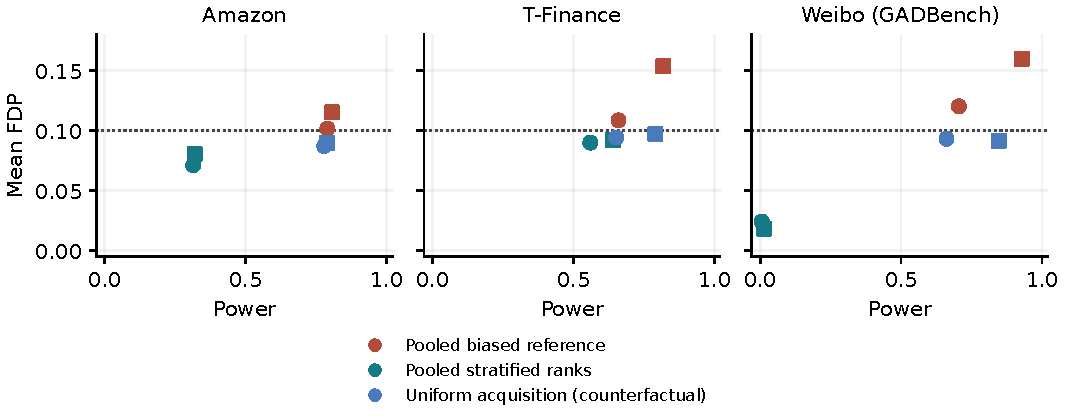
\includegraphics[width=\textwidth]{acquisition_main.pdf}
\caption{Correction can reduce FDP while sacrificing useful discoveries. Training labels define the 80/20 exposure strata; acquisition probabilities are $0.50$ and $0.10$ in the lower and upper strata. Circles denote attribute scorers and squares graph-feature scorers. All three graphs are shown, including Weibo's nearly powerless stratified result. The blue reference is a counterfactual uniform-acquisition design at comparable expected label cost, not an available reference in the biased scenario. Points average ten seed means; the dotted line marks nominal $0.10$. Figure~\ref{fig:allocationfull} and Appendix~\ref{app:allocation} retain every allocation, weighting and acquisition-severity comparison.}
\label{fig:allocation}
\end{figure*}

\clearpage\section{PAIRED UNCERTAINTY OVER THE COMPLETE DOSE GRID}
For each training seed, subtract random-removal FDP (or power) from the corresponding exposure-removal value after averaging its five test splits and fifty calibration repetitions. Report the mean of ten paired differences and the pointwise interval $\bar d\pm t_{9,.975}s_d/\sqrt{10}$. This estimates repeated-training/evaluation uncertainty on the given graph, not variation across graphs. The intervals are pointwise and do not adjust for searching across conditions. The complete grid is shown rather than retaining only positive intervals.
\begin{figure*}[t]\centering
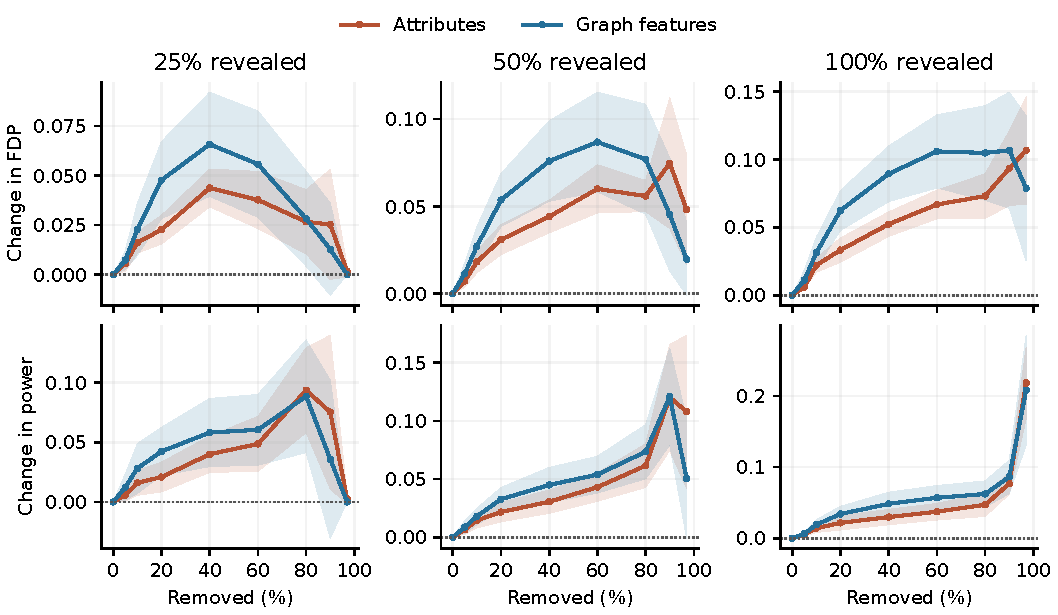
\includegraphics[width=\textwidth]{dose_paired_amazon.pdf}
\caption{Amazon: exposure removal minus size-matched random removal over the complete dose grid. Shading gives pointwise 95\% paired $t$ intervals across ten training-seed averages after averaging splits and calibration repetitions. Intervals describe repeated evaluation conditional on this graph; they are neither simultaneous across the sweep nor uncertainty over new graphs.}
\end{figure*}

\begin{figure*}[t]\centering
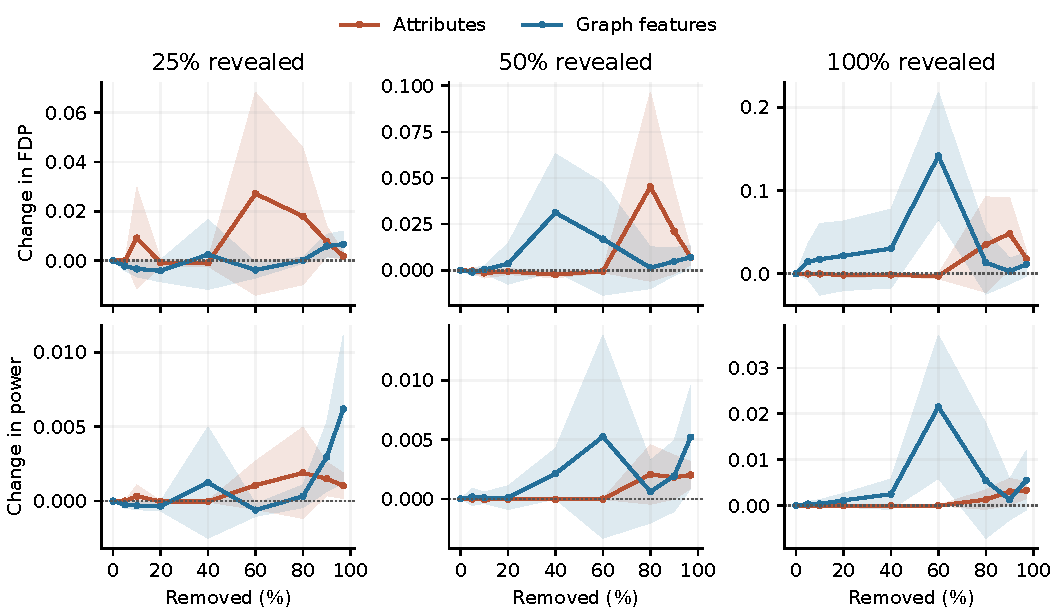
\includegraphics[width=\textwidth]{dose_paired_tolokers.pdf}
\caption{Tolokers: exposure removal minus size-matched random removal over the complete dose grid. Shading gives pointwise 95\% paired $t$ intervals across ten training-seed averages after averaging splits and calibration repetitions. Intervals describe repeated evaluation conditional on this graph; they are neither simultaneous across the sweep nor uncertainty over new graphs.}
\end{figure*}

\begin{figure*}[t]\centering
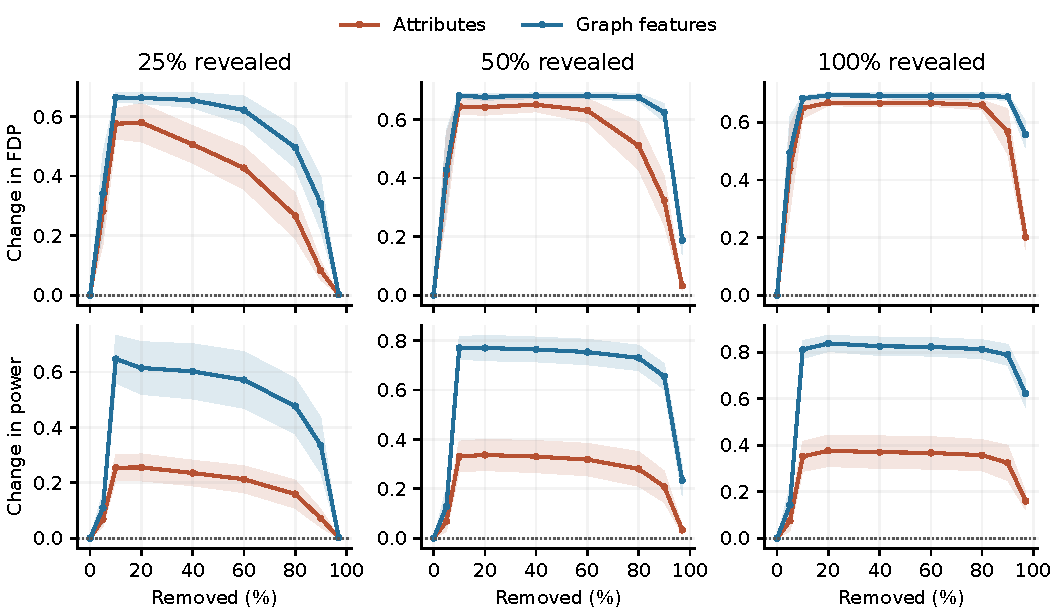
\includegraphics[width=\textwidth]{dose_paired_weibo.pdf}
\caption{Weibo (PyGOD): exposure removal minus size-matched random removal over the complete dose grid. Shading gives pointwise 95\% paired $t$ intervals across ten training-seed averages after averaging splits and calibration repetitions. Intervals describe repeated evaluation conditional on this graph; they are neither simultaneous across the sweep nor uncertainty over new graphs.}
\end{figure*}

\begin{figure*}[t]\centering
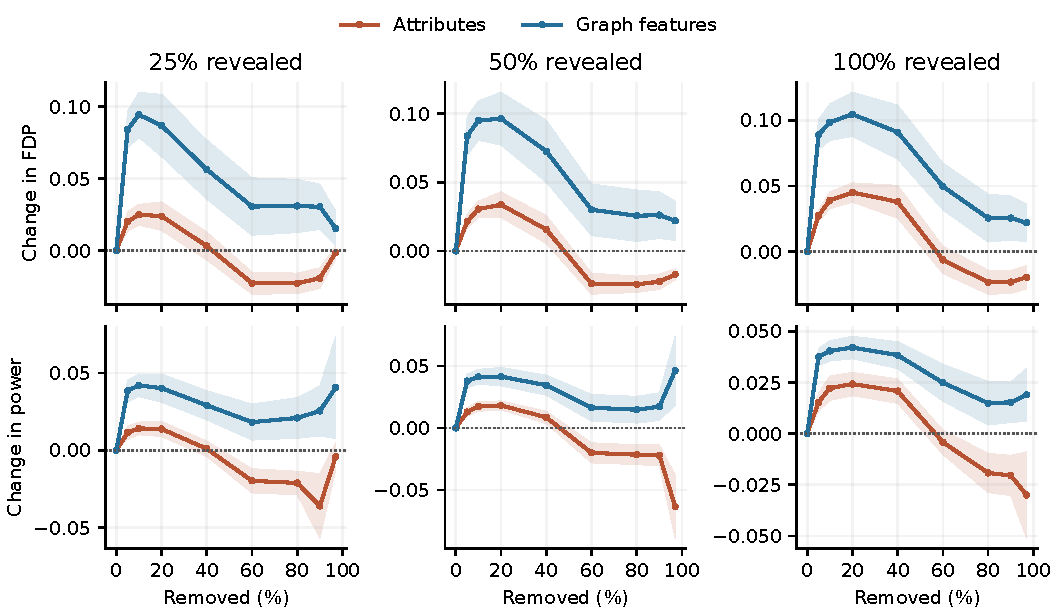
\includegraphics[width=\textwidth]{dose_paired_tfinance.pdf}
\caption{T-Finance: exposure removal minus size-matched random removal over the complete dose grid. Shading gives pointwise 95\% paired $t$ intervals across ten training-seed averages after averaging splits and calibration repetitions. Intervals describe repeated evaluation conditional on this graph; they are neither simultaneous across the sweep nor uncertainty over new graphs.}
\end{figure*}

\begin{figure*}[t]\centering
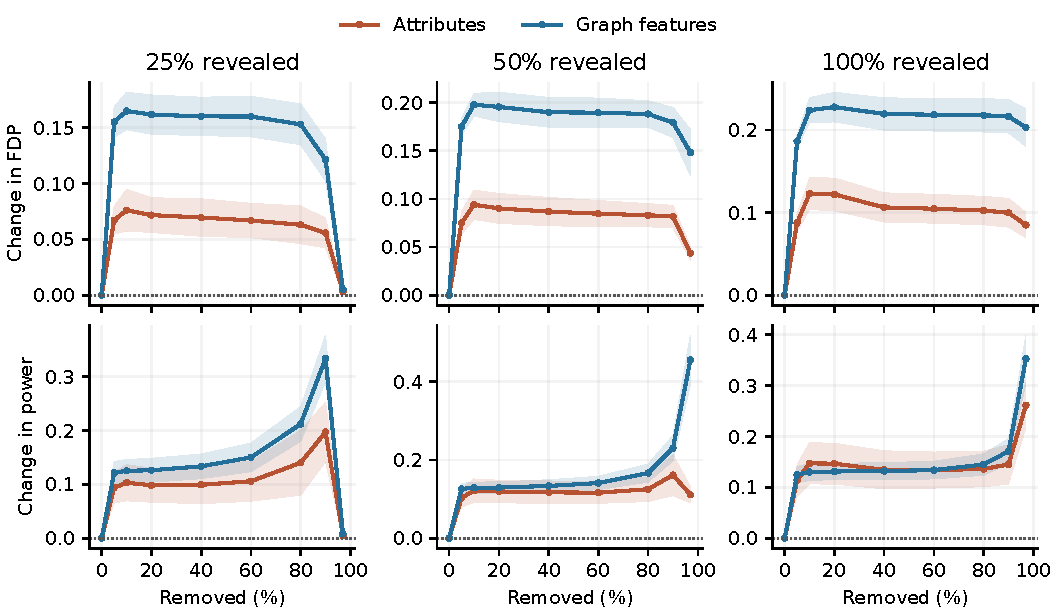
\includegraphics[width=\textwidth]{dose_paired_weibo_gadbench.pdf}
\caption{Weibo (GADBench): exposure removal minus size-matched random removal over the complete dose grid. Shading gives pointwise 95\% paired $t$ intervals across ten training-seed averages after averaging splits and calibration repetitions. Intervals describe repeated evaluation conditional on this graph; they are neither simultaneous across the sweep nor uncertainty over new graphs.}
\end{figure*}

\clearpage\section{UNSUPERVISED COMPARISONS}
\label{app:unsupervised}
\begin{figure*}[t]
\centering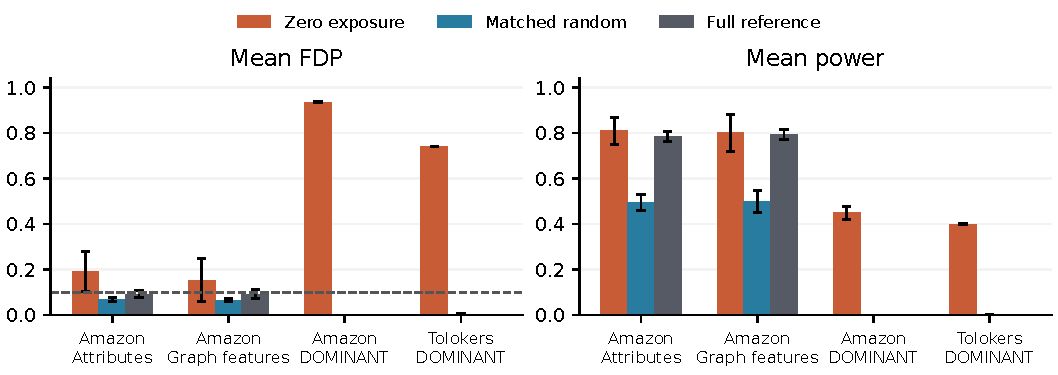
\includegraphics[width=\textwidth]{headline_results.pdf}
\caption{Reference composition changes FDP (left) and power (right) differently. Each panel compares accurate supervised Amazon scorers with DOMINANT on Amazon and Tolokers. Bars show seed means; error bars are one seed SD, not confidence intervals over new graphs. Filtered and random references are matched in size; full references are larger. The horizontal line marks nominal $0.10$ in the FDP panel. Low FDP with zero power is distinguished from useful discovery.}
\label{fig:headline}
\end{figure*}
\begin{table*}[ht]\centering\small
\caption{Untrimmed, verified-label comparisons. FDP and power are means $\pm$ SD of ten seed averages, each averaged across five test splits and calibration repetitions. All zero-discovery outcomes are retained.}
\label{tab:untrimmed}\begin{tabular}{lllrrrr}\toprule
Graph & Detector & Rule & Mean $n$ & FDP & Power & AUROC\\\midrule
Amazon & DOMINANT & Filtered & 162 & $0.9357\pm0.0034$ & $0.4489\pm0.0299$ & 0.340 \\
Amazon & DOMINANT & Random & 162 & $0.0000\pm0.0000$ & $0.0000\pm0.0000$ & 0.340 \\
Amazon & GAE & Filtered & 162 & $0.0000\pm0.0000$ & $0.0000\pm0.0000$ & 0.866 \\
Amazon & GAE & Random & 162 & $0.0014\pm0.0009$ & $0.0008\pm0.0006$ & 0.866 \\
Amazon & Isolation Forest & Filtered & 162 & $0.0000\pm0.0000$ & $0.0000\pm0.0000$ & 0.840 \\
Amazon & Isolation Forest & Random & 162 & $0.0003\pm0.0005$ & $0.0001\pm0.0001$ & 0.840 \\
Tolokers & DOMINANT & Filtered & 621 & $0.7400\pm0.0007$ & $0.3983\pm0.0021$ & 0.530 \\
Tolokers & DOMINANT & Random & 621 & $0.0038\pm0.0013$ & $0.0004\pm0.0001$ & 0.530 \\
Tolokers & GAE & Filtered & 621 & $0.0000\pm0.0000$ & $0.0000\pm0.0000$ & 0.431 \\
Tolokers & GAE & Random & 621 & $0.0000\pm0.0000$ & $0.0000\pm0.0000$ & 0.431 \\
Tolokers & Isolation Forest & Filtered & 621 & $0.0000\pm0.0000$ & $0.0000\pm0.0000$ & 0.397 \\
Tolokers & Isolation Forest & Random & 621 & $0.0000\pm0.0000$ & $0.0000\pm0.0000$ & 0.397 \\
\bottomrule\end{tabular}

\end{table*}
Unsupervised comparisons use DOMINANT, PyGOD attribute-reconstruction GAE, and Isolation Forest, plus positive degree as an untrained control. The neural models use width 64, four layers, no dropout, and 100 full-batch Adam steps at learning rate $0.01$; Isolation Forest uses 200 trees and subsample size 256. Model settings and score directions are fixed. Ten training seeds share five stratified test splits. Graph features are transductive; evaluation labels are not reconstruction targets. The zero-exposure oracle retains reference normals with no anomalous neighbors; matched random calibration draws equally many reference normals, capped at 1,000, and a full-reference arm uses every eligible normal. The partial-label filter uses known training labels and a random revealed fraction $\rho\in\{0.25,0.50\}$ of non-test deployment labels. We use 200 calibration repetitions per matched comparison.

For DOMINANT, zero-exposure filtering gives FDP $0.936$ on Amazon and $0.740$ on Tolokers, with powers $0.449$ and $0.398$. Matched random calibration has FDP $0$ and $0.004$, with essentially zero power. DOMINANT AUROCs are $0.340$ and $0.530$, so those contrasts do not describe a useful calibrated detector. GAE and Isolation Forest make no oracle-filtered discoveries on either graph; full-reference calibration makes none for any of the three original scorers. Positive degree alone, fixed before evaluation, has AUROC $0.221$ on Amazon and $0.560$ on Tolokers; its filtered mean FDP is $0.955$ and $0.758$, so learned message passing is unnecessary for this particular failure. With 25\% of non-test labels revealed, DOMINANT filtered FDP is $0.973$ and $0.721$; with 50\%, it is $0.964$ and $0.726$. These scores have low power under random calibration. Table~\ref{tab:partial} reports the full FDP--power comparisons. Reference-only trimming and enriched test populations are separate sensitivity interventions in Table~\ref{tab:trim}, not definitions of the primary population.

\section{COMPLETE FOLLOW-UP COMPARISONS}
\label{app:followup}
\begin{table*}[t]
\centering\small
\caption{Untrimmed DOMINANT comparisons, reported as mean FDP / power across all ten seeds, five splits, and 200 calibration draws. The 25\% and 50\% rows reveal only non-test labels. The 100\% row is the oracle intervention, which can use test-neighbor labels. Mixture composition is fixed in advance.}
\label{tab:partial}\begin{tabular}{llrrr}\toprule
Graph & Labels (\%) & Filtered & Random & Half mixture\\\midrule
Amazon & 25 & 0.9733 / 0.0942 & 0.0000 / 0.0000 & 0.0005 / 0.0000 \\
Amazon & 50 & 0.9635 / 0.1895 & 0.0000 / 0.0000 & 0.0019 / 0.0000 \\
Amazon & 100 & 0.9357 / 0.4489 & 0.0000 / 0.0000 & 0.0039 / 0.0001 \\
Tolokers & 25 & 0.7205 / 0.3358 & 0.0079 / 0.0010 & 0.0329 / 0.0046 \\
Tolokers & 50 & 0.7262 / 0.3552 & 0.0047 / 0.0005 & 0.0342 / 0.0041 \\
Tolokers & 100 & 0.7400 / 0.3983 & 0.0038 / 0.0004 & 0.0362 / 0.0049 \\
\bottomrule\end{tabular}

\end{table*}
\begin{table*}[t]
\centering\small
\caption{DOMINANT trimming and target-population sensitivity. Natural-prevalence reference-only trimming preserves test identities. Enriched-test rows include every anomaly and 2,000 normal test nodes; trimming both pools can also change test identities and reference size. Amazon uses verified labels throughout this table. All entries average ten seeds, five splits, and 200 calibration draws.}
\label{tab:trim}\begin{tabular}{llrrrrr}\toprule
Graph & Test / trimming design & Trim (\%) & Filter FDP & Power & Random FDP & Power\\\midrule
Amazon & Natural, no trim & 0 & 0.9357 & 0.4489 & 0.0000 & 0.0000 \\
Amazon & Natural, reference trim & 1 & 0.9357 & 0.4489 & 0.0000 & 0.0000 \\
Amazon & Natural, reference trim & 5 & 0.9357 & 0.4489 & 0.0593 & 0.0007 \\
Amazon & Enriched, both pools & 0 & 0.7916 & 0.4373 & 0.0000 & 0.0000 \\
Amazon & Enriched, both pools & 1 & 0.7945 & 0.4245 & 0.0000 & 0.0000 \\
Amazon & Enriched, both pools & 5 & 0.7844 & 0.4429 & 0.0000 & 0.0000 \\
Tolokers & Natural, no trim & 0 & 0.7400 & 0.3983 & 0.0038 & 0.0004 \\
Tolokers & Natural, reference trim & 1 & 0.7400 & 0.3983 & 0.4271 & 0.0575 \\
Tolokers & Natural, reference trim & 5 & 0.7400 & 0.3983 & 0.6036 & 0.1369 \\
Tolokers & Enriched, both pools & 0 & 0.3936 & 0.3749 & 0.0200 & 0.0052 \\
Tolokers & Enriched, both pools & 1 & 0.3913 & 0.3815 & 0.0369 & 0.0583 \\
Tolokers & Enriched, both pools & 5 & 0.3608 & 0.3654 & 0.0462 & 0.1330 \\
\bottomrule\end{tabular}

\end{table*}
Complete comparison outputs include both reference budgets, all learned detectors, the positive-degree control, and declared sensitivity conditions. Their seed SDs and split-average ranges describe repeated evaluation of fixed graphs. The ten-seed DOMINANT protocol and the subsequent GPU GAE extension were fixed before their respective outcomes were inspected.

\clearpage\section{SUPERVISED CONTROLS AND REFERENCE BUDGET}
\label{app:supervised}
The following experiments were specified after inspecting the original cached-score results. They are exploratory robustness checks, not independent confirmatory evidence on new graph instances. Every graph, model, seed, and declared label budget is retained, including negative results. The scripts, protocols, score caches, per-draw results, and checks are supplied under \texttt{paper/audit\_method}.

\paragraph{Training and evaluation.}
For each of ten seeds, draw a uniform 10\% sample of verified nodes without inspecting its labels. This gives 864 training labels on Amazon and 1,176 on Tolokers. Remaining deployment sizes are 7,775 and 10,582. Fit scikit-learn's histogram-gradient-boosting classifier with 200 iterations, learning rate $0.1$, at most 31 leaves, minimum leaf size 20, $L_2$ regularization 1, no class weighting, and no early stopping. The attribute model uses the cached features. The graph model adds the unweighted one-hop feature mean and $\log(1+d)$. These covariates use no labels; graph training features may incorporate unlabeled test-node attributes, consistent with the transductive setting. Training labels are not reused as calibration or certification observations. No hyperparameter or score-direction selection uses deployment outcomes.

Each training panel uses five label-stratified splits of the remaining deployment population, with approximately 25\% assigned to testing. Splits are paired between scorers but vary across training panels; this differs from the crossed seed--split design of the unsupervised replication. For each split, the oracle filter uses all anomalous-neighbor labels, and the matched random comparator draws 200 samples at the filtered pool size. Filtered pools never exceed the declared cap of 1,000, so that rule selects the entire filtered pool. Full-reference calibration includes all eligible non-test normals. Table~\ref{tab:supervisedfull} reports seed means and SDs after averaging over calibration draws and splits. The reference pool is normal-only; obtaining it requires labeling the reference panel, rather than knowing normal identities for free.

\begin{table*}[t]
\centering\scriptsize
\caption{Complete supervised oracle-filter comparison. FDP and power are mean $\pm$ SD of ten training-seed averages; discoveries and calibration size $n$ are means. Full-reference and matched comparisons share test sets but differ in reference size.}
\label{tab:supervisedfull}\begin{tabular}{lllrrrr}
\toprule
Graph & Score & Reference & $n$ & FDP & Power & Discoveries \\
\midrule
Amazon & Attributes & Filtered & 143.2 & $0.192\pm0.087$ & $0.809\pm0.060$ & 193.9 \\
Amazon & Attributes & Full reference & 5275.5 & $0.092\pm0.016$ & $0.783\pm0.022$ & 160.0 \\
Amazon & Attributes & Matched random & 143.2 & $0.067\pm0.009$ & $0.495\pm0.034$ & 103.5 \\
Amazon & Attributes + graph & Filtered & 143.2 & $0.154\pm0.094$ & $0.801\pm0.081$ & 180.0 \\
Amazon & Attributes + graph & Full reference & 5275.5 & $0.091\pm0.019$ & $0.793\pm0.022$ & 161.9 \\
Amazon & Attributes + graph & Matched random & 143.2 & $0.066\pm0.008$ & $0.500\pm0.049$ & 104.3 \\
Tolokers & Attributes & Filtered & 559.9 & $0.065\pm0.092$ & $0.004\pm0.006$ & 6.0 \\
Tolokers & Attributes & Full reference & 6203.7 & $0.000\pm0.000$ & $0.000\pm0.000$ & 0.0 \\
Tolokers & Attributes & Matched random & 559.9 & $0.000\pm0.000$ & $0.000\pm0.000$ & 0.0 \\
Tolokers & Attributes + graph & Filtered & 559.9 & $0.005\pm0.015$ & $0.001\pm0.004$ & 1.0 \\
Tolokers & Attributes + graph & Full reference & 6203.7 & $0.026\pm0.043$ & $0.001\pm0.002$ & 0.7 \\
Tolokers & Attributes + graph & Matched random & 559.9 & $0.005\pm0.003$ & $0.001\pm0.001$ & 0.7 \\
\bottomrule
\end{tabular}

\end{table*}

\paragraph{Filtering with observed non-test labels.}
Reveal each non-test deployment node with probability $\rho\in\{0.25,0.50\}$ using nested random draws. All training labels are already known and may identify anomalous neighbors, but training nodes remain excluded from calibration. The eligible reference consists only of revealed normal deployment nodes. A node passes the filter if no known anomalous neighbor occurs in either the training or revealed reference panel. Both filtered and random rules draw $\min(1000,|\mathcal P_F|)$ nodes, with 200 repetitions; the full-reference arm uses the entire revealed normal pool. Changing every unknown label leaves the filter unchanged in all 200 graph--seed--split--revelation checks. Labels used to construct stratified benchmark test sets and calculate FDP are never passed to the filter.

\begin{table*}[t]
\centering\scriptsize
\caption{All supervised partial-label comparisons. FDP and power are mean $\pm$ seed SD. ``Labels'' counts the mean revealed non-test deployment labels, including normal and anomalous nodes; add 864 training labels for Amazon or 1,176 for Tolokers. Thus these comparisons are not equal-label-budget alternatives to direct batch certification.}
\label{tab:supervisedpartial}\begin{tabular}{llrlrrr}
\toprule
Graph & Score & $\rho$ & Reference & FDP & Power & Labels \\
\midrule
Amazon & Attributes & 0.25 & Filtered & $0.093\pm0.047$ & $0.679\pm0.113$ & 1467 \\
Amazon & Attributes & 0.25 & Full reference & $0.091\pm0.019$ & $0.779\pm0.015$ & 1467 \\
Amazon & Attributes & 0.25 & Matched random & $0.063\pm0.010$ & $0.591\pm0.047$ & 1467 \\
Amazon & Attributes & 0.50 & Filtered & $0.140\pm0.069$ & $0.770\pm0.061$ & 2923 \\
Amazon & Attributes & 0.50 & Full reference & $0.089\pm0.016$ & $0.779\pm0.018$ & 2923 \\
Amazon & Attributes & 0.50 & Matched random & $0.069\pm0.009$ & $0.622\pm0.035$ & 2923 \\
Amazon & Attributes + graph & 0.25 & Filtered & $0.085\pm0.038$ & $0.675\pm0.077$ & 1467 \\
Amazon & Attributes + graph & 0.25 & Full reference & $0.089\pm0.025$ & $0.778\pm0.018$ & 1467 \\
Amazon & Attributes + graph & 0.25 & Matched random & $0.065\pm0.013$ & $0.601\pm0.067$ & 1467 \\
Amazon & Attributes + graph & 0.50 & Filtered & $0.118\pm0.064$ & $0.756\pm0.084$ & 2923 \\
Amazon & Attributes + graph & 0.50 & Full reference & $0.091\pm0.022$ & $0.791\pm0.018$ & 2923 \\
Amazon & Attributes + graph & 0.50 & Matched random & $0.072\pm0.011$ & $0.626\pm0.034$ & 2923 \\
Tolokers & Attributes & 0.25 & Filtered & $0.028\pm0.059$ & $0.002\pm0.004$ & 1987 \\
Tolokers & Attributes & 0.25 & Full reference & $0.009\pm0.030$ & $0.000\pm0.001$ & 1987 \\
Tolokers & Attributes & 0.25 & Matched random & $0.001\pm0.002$ & $0.000\pm0.000$ & 1987 \\
Tolokers & Attributes & 0.50 & Filtered & $0.057\pm0.101$ & $0.003\pm0.005$ & 3978 \\
Tolokers & Attributes & 0.50 & Full reference & $0.000\pm0.000$ & $0.000\pm0.000$ & 3978 \\
Tolokers & Attributes & 0.50 & Matched random & $0.001\pm0.001$ & $0.000\pm0.000$ & 3978 \\
Tolokers & Attributes + graph & 0.25 & Filtered & $0.000\pm0.000$ & $0.000\pm0.000$ & 1987 \\
Tolokers & Attributes + graph & 0.25 & Full reference & $0.010\pm0.022$ & $0.001\pm0.002$ & 1987 \\
Tolokers & Attributes + graph & 0.25 & Matched random & $0.003\pm0.003$ & $0.001\pm0.001$ & 1987 \\
Tolokers & Attributes + graph & 0.50 & Filtered & $0.005\pm0.015$ & $0.001\pm0.004$ & 3978 \\
Tolokers & Attributes + graph & 0.50 & Full reference & $0.023\pm0.035$ & $0.001\pm0.002$ & 3978 \\
Tolokers & Attributes + graph & 0.50 & Matched random & $0.005\pm0.003$ & $0.001\pm0.001$ & 3978 \\
\bottomrule
\end{tabular}

\end{table*}

\paragraph{Unrestricted references and degree normalization.}
On the original corrected, untrimmed score caches, full-reference calibration uses 5,864 normals on Amazon and 6,894 on Tolokers. All 400 configurations (two graphs, four scores, ten seeds, five splits) produce no discoveries. The four scores are DOMINANT, GAE, Isolation Forest, and DOMINANT divided by $\log(1+d+10^{-8})$. This fixed normalization gives Amazon AUROC $0.536$ and filtered mean FDP $0.165$ (seed SD $0.182$), with power $0.061$ (SD $0.071$). Its matched random mean FDP is $0.000085$ and power $0.000009$; all Tolokers normalized-score rules make no discoveries. Normalization changes the score ranking and reduces one contrast, but does not yield a useful calibrated detector here or identify degree as the unique cause.

\paragraph{Reproducibility.}
Master seeds 20260924--20260926 define the supervised training panels, certification audits, and evaluation splits; 20260928 defines the observed-label checks. The output contains 40 trained score vectors, 40,400 supervised oracle-comparison rows, and 160,400 observed-label comparison rows. Input and output checksums, software versions, train/deployment separation, matching of reference sizes, and complete seed coverage are checked in the supplied scripts. Monte Carlo draws on the same graph are not independent graph replications.

\clearpage
\section{EXPLORATORY FIXED-BATCH FDP CERTIFICATION}
\label{app:certificate}
The conditional rank audit in the main text diagnoses a reference-sampling rule using known benchmark labels. A different task is to certify the precision of proposed discoveries by obtaining a random audit of their labels. We examine a standard finite-population construction for that task. Simultaneous risk certification is closely related to Learn then Test~\citep{angelopoulos2022ltt}; exact hypergeometric inversion and certification of fixed candidate families also appear in recent work on candidate-generation coverage~\citep{anthony2026audits}. The latter targets missed mass and recall rather than the FDP of unreviewed discoveries. We claim neither a new confidence-bound principle nor superiority of the evaluated graph-stratified design.

\paragraph{Procedure and guarantee.}
Condition on a finite graph, its binary labels, a trained scorer, and $K$ candidate sets fixed before audit labels are obtained. Audit uniformly without replacement from a fixed superset of these candidates. Conditional on the number $h_k$ of audited nodes in candidate $k$ of size $R_k$, the observed normal count $X_k$ is hypergeometric with unknown total normal count $V_k$. Write $H_{R,v,h}(x)$ for its CDF and define
\[
 U_k(x)=\max\{v:H_{R_k,v,h_k}(x)\ge\delta/K\},
\]
where the maximum ranges over integers $x\le v\le R_k-h_k+x$. Remove every audited node from automatic discoveries. For $R_k>h_k$, its remaining FDP has upper bound
\[
 B_k=\frac{\min\{R_k-h_k,U_k(X_k)-X_k\}}{R_k-h_k}.
\]
Select the largest remaining candidate with $B_k\le q$, or abstain if none qualifies. This permits data-dependent choice among the fixed candidates, not tuning the candidates or scorer using the audit labels.

For completeness, the hypergeometric CDF decreases in $v$. Hence $U_k(X_k)<V_k$ implies $H_{R_k,V_k,h_k}(X_k)<\delta/K$, an event with probability at most $\delta/K$ by discrete CDF super-uniformity. Conditioning on $h_k$ and then averaging preserves this bound. A union bound makes all $K$ normal-count bounds hold with probability at least $1-\delta$, without independent candidates or independent graph nodes. Subtracting the observed audited normals gives the displayed FDP bounds simultaneously. Consequently the selected unreviewed set satisfies
\[
 \Prb_{\rm audit}\{\FDP\le q\}\ge1-\delta.
\]
Correct labels and the specified random audit design are essential. This certifies the fixed batch, not future graphs. It implies $\E[\FDP]\le q+(1-q)\delta$; at $q=0.10,\delta=0.05$ this is $0.145$, not $0.10$. Scorer selection after audit inspection would require joint coverage over the model family; our comparisons evaluate frozen scorers separately.

\paragraph{Designs and budgets.}
Use candidate score prefixes of sizes $25,50,100,200,400,800,1600,\lfloor0.2N\rfloor$, sorted and deduplicated, with node ID breaking score ties. $N$ is the entire deployment batch rather than the smaller conformal test split. Uniform auditing samples either the largest candidate or the whole deployment graph. Score stratification partitions the largest candidate at the prefix boundaries. Degree stratification further divides each score band into equal-size degree-rank halves. Capped equal allocation assigns the fixed budget to strata before observing labels. Each stratum receives a hypergeometric upper bound at level $\delta/H$, where $H$ is the number of strata; summing these bounds over complete candidate strata and subtracting observed normals gives the same simultaneous FDP guarantee. This allocation is a prototype, not an optimized sampling rule.

For every frozen score, evaluate budgets $B\in\{100,250,500\}$ with 200 audits per design at $q=0.10,\delta=0.05$. With the original three detectors and normalized DOMINANT, all 192,000 audit trials abstain. The declared prefixes lack the population precision needed for useful 90\%-precision certification in that score regime. The subsequent supervised extension uses 96,000 audit trials and separately accounts for training labels. Its full mean true-discovery comparison is in Table~\ref{tab:certificate}; all omitted smaller-budget stratified and whole-graph cells are zero, and the supplied CSV contains every cell.

\begin{table*}[t]
\centering\scriptsize
\caption{Mean true discoveries among unreviewed nodes. All 100- and 250-label cells for score strata, score-plus-degree strata, and graph-uniform auditing are zero. Means include abstention; audited anomalies are excluded. Each entry averages ten trained scorers and 200 audits per scorer.}
\label{tab:certificate}\begin{tabular}{llrrrrrr}
\toprule
Graph & Score & \multicolumn{3}{c}{Candidate uniform} & Score strata & Score + degree & Graph uniform \\
 & & $B=100$ & $B=250$ & $B=500$ & $B=500$ & $B=500$ & $B=500$ \\
\midrule
Amazon & Attributes & 0.0 & 87.0 & 211.5 & 4.7 & 0.0 & 0.0 \\
Amazon & Attributes + graph & 0.0 & 86.3 & 202.8 & 10.2 & 0.0 & 0.0 \\
Tolokers & Attributes & 0.0 & 0.0 & 0.0 & 0.0 & 0.0 & 0.0 \\
Tolokers & Attributes + graph & 0.0 & 0.0 & 0.0 & 0.0 & 0.0 & 0.0 \\
\bottomrule
\end{tabular}

\end{table*}

Amazon's attribute model with 500 candidate-uniform audit labels returns mean 216.0 automatic discoveries, of which 211.5 are true. It returns a nonempty set in 80.75\% of trials; mean FDP is $0.0165$ including abstention and $0.0204$ conditional on a nonempty set. Its 864 training labels are additional to the audit budget. The graph-feature scorer gives mean 207.4 automatic discoveries, including 202.8 true anomalies. Degree stratification and whole-graph uniform auditing return none; score-only stratification returns substantially fewer. Every Tolokers condition abstains. Thus direct certification is useful in one accurate-score regime, but the present graph-stratified allocation does not improve label efficiency.

\paragraph{Validation.}
Exact enumeration checks 18,600 hypergeometric coverage cases and 2,048 small-population selection configurations, including nonempty selection, full and empty audits, and all-normal/all-anomaly populations. A further 64,000 synthetic audits include nonvacuous high-precision controls; the largest observed cell failure rate is $0.005$ at $\delta=0.05$. No supervised-score audit violates the FDP target in these runs. These implementation checks supplement the proof; neither zero observed violations nor the large number of reused-graph audits supplies the guarantee.


\clearpage\section{IMPLEMENTATION AND REPRODUCIBILITY}
\label{app:implementation}
The supplement contains the code, frozen protocols, cached detector scores, per-trial result ledgers and summaries behind every table and figure, together with a script that checks every file against a hash manifest, recomputes every weighted-selection summary from its per-trial ledger, reruns the exact finite-design validations, reruns the Amazon acquisition experiments from the cached scores and compares them with the shipped outcomes, and regenerates the result tables. On a laptop CPU the default check takes a few minutes and the full check, which also retrains the Amazon scorers on the biased labels, about twenty minutes. Every random stream is seeded with \texttt{numpy.random.SeedSequence}. In our environment, with the versions listed below, the verification script reproduced the shipped outcomes exactly from a fresh copy; other library versions or hardware may introduce small numerical differences.

The primary GPU batch for the unsupervised detectors contains 60 model--seed configurations and two fixed degree controls, producing 2,325,000 calibration-method evaluations. Every stored summary mean was recomputed from its per-draw CSV, and all 60 job checksum manifests were verified after download. Training used Python 3.13.14, PyTorch 2.13.0+cu126, PyG 2.8.0, PyGOD 1.1.0, and one NVIDIA H200 NVL, with TF32 disabled. CPU and GPU results are not pooled. The supervised scorers, the removal sweeps, and all weighted-selection experiments run on a CPU with Python 3.14.2, NumPy 2.5.0, SciPy 1.18.0, pandas 3.0.5 and scikit-learn 1.9.0. Experiments use synthetic data and public graph benchmarks; no new human-subject data were collected.

\begin{table}[ht]
\centering\small\setlength{\tabcolsep}{4pt}
\caption{Neural-model settings for the unsupervised graph comparisons.}
\begin{tabular}{ll}
\toprule Setting & Value\\\midrule
Scoring library & PyGOD 1.1.0 modules\\
Hidden width / layers & 64 / 4\\
Dropout & 0\\
Optimization & Full-batch Adam\\
Learning rate / epochs & 0.01 / 100\\
Early stopping & None\\
Feature scaling & Graph column standardization\\
Nominal BH level & 0.10\\
Training seeds & 10\\
Score trimming & None\\
Test fraction & 25\% stratified\\
Reference budget & 200 and 1,000\\
\bottomrule
\end{tabular}
\end{table}
The model interface uses PyGOD's \texttt{DOMINANTBase} and \texttt{GAEBase} with explicit full-batch training loops, not the high-level neighbor-sampling API. The GAE score is the sum of squared attribute reconstruction errors. PyGOD traces its GAE family to \citet{kipf2016variational}; our deterministic attribute-decoder configuration is not the variational adjacency-reconstruction model of that paper. DOMINANT uses its module's per-node attribute/structure loss. Both models are trained on standardized features and an undirected representation of the loaded graph. Relation types in Amazon are collapsed into a common graph. Labels are used in selection and evaluation, not as reconstruction targets. Scores and test identities are shared within each matched comparison. Repeated calibration draws quantify sampling variation conditional on a graph; seed SDs summarize training variability on that same graph.
\end{document}
